% Copyright 2004 by Till Tantau <tantau@users.sourceforge.net>.
%
% In principle, this file can be redistributed and/or modified under
% the terms of the GNU Public License, version 2.
%
% However, this file is supposed to be a template to be modified
% for your own needs. For this reason, if you use this file as a
% template and not specifically distribute it as part of a another
% package/program, I grant the extra permission to freely copy and
% modify this file as you see fit and even to delete this copyright
% notice. 
\documentclass{beamer}
\usepackage{bbm}
\usepackage{lipsum}
\usepackage{enumitem}
\usepackage{pifont}
\logo{\color{red}\rule{.5cm}{.5cm}}

%\usepackage{xcolor}
%\usepackage{tikz}
%\usetikzlibrary{shadows}
\newlength{\tmpShadow}
\newcommand{\MyShadow}[2]{%
	\settowidth{\tmpShadow}{#1}
	\addtolength{\tmpShadow}{.1em}
	\raisebox{-0.25ex}{\textcolor{gray!70}{#1}}%
	\kern-\tmpShadow%
	\textcolor{#2}{#1}%
}
%\newcommand*{\MyShadowBullet}{\tikz \draw [baseline, fill=blue,draw=blue,circular drop shadow] circle (2pt);}
%\newcommand*{\MyBallBullet}{\tikz \draw [baseline, ball color=red, draw=red] circle (2pt);}

\newcommand{\nologo}{\setbeamertemplate{logo}{}} % command to set the logo to nothing
\usepackage{multicol}
\newcommand\tab[1][1cm]{\hspace*{#1}}

%gets rid of bottom navigation bars
%\setbeamertemplate{footline}[frame number]{}
%gets rid of bottom navigation symbols
\setbeamertemplate{navigation symbols}{}
%gets rid of footer
%will override 'frame number' instruction above
%comment out to revert to previous/default definitions
%\setbeamertemplate{footline}{}

\newcounter{mycounter}  
\newenvironment{noindlist}
{\begin{list}{}{\usecounter{mycounter} \labelsep=0em \labelwidth=0em \leftmargin=0em \itemindent=0em}}
	{\end{list}}

% There are many different themes available for Beamer. A comprehensive
% list with examples is given here:
% http://deic.uab.es/~iblanes/beamer_gallery/index_by_theme.html
% You can uncomment the themes below if you would like to use a different
% one:
%\usetheme{AnnArbor}
%\usetheme{Antibes}
%\usetheme{Bergen}
%\usetheme{Berkeley}
%\usetheme{Berlin}
%\usetheme{Boadilla}
%\usetheme{boxes}
%\usetheme{CambridgeUS}
%\usetheme{Copenhagen}
%\usetheme{Darmstadt}
%\usetheme{default}
%\usetheme{Frankfurt}
%\usetheme{Goettingen}
%\usetheme{Hannover}
%\usetheme{Ilmenau}
%\usetheme{JuanLesPins}
%\usetheme{Luebeck}
\usetheme{Madrid}
%\usetheme{Malmoe}
%\usetheme{Marburg}
%\usetheme{Montpellier}
%\usetheme{PaloAlto}
%\usetheme{Pittsburgh}
%\usetheme{Rochester}
%\usetheme{Singapore}
%\usetheme{Szeged}
%\usetheme{Warsaw}

\title{Behavioural pattern recognition of animal paths obtained from experimental procedures}

% A subtitle is optional and this may be deleted
%\subtitle{Optional Subtitle}

\author{Avgoustinos~Vouros\inst{1}}
% - Give the names in the same order as the appear in the paper.
% - Use the \inst{?} command only if the authors have different
%   affiliation.

\institute[] % (optional, but mostly needed)
{
  \inst{1}%
  PhD student, \\Department of Computer Science,\\
  University of Sheffield\\
  \vspace{5mm}
  \noindent Supervised by Prof Eleni Vasilaki
  %\and
  %\inst{2}%
  %Department of Theoretical Philosophy\\
  %University of Elsewhere
}

\date{} %removes the date
% - Use the \inst command only if there are several affiliations.
% - Keep it simple, no one is interested in your street address.

%\date{Conference Name, 2013}
% - Either use conference name or its abbreviation.
% - Not really informative to the audience, more for people (including
%   yourself) who are reading the slides online

%\subject{Theoretical Computer Science}
% This is only inserted into the PDF information catalog. Can be left
% out. 

% If you have a file called "university-logo-filename.xxx", where xxx
% is a graphic format that can be processed by latex or pdflatex,
% resp., then you can add a logo as follows:

\pgfdeclareimage[height=1cm]{university-logo}{university-logo}
\logo{\pgfuseimage{university-logo}}

% Delete this, if you do not want the table of contents to pop up at
% the beginning of each subsection:
\AtBeginSubsection[]
{
  \begin{frame}<beamer>{Outline}
    \tableofcontents[]
  \end{frame}
}

% Let's get started
\begin{document}

\begin{frame}
  \titlepage
\end{frame}

%\begin{frame}{Acknowledgements}
%	Original slides created by: 
%	\begin{itemize}
%		\item Eleni Vasilaki (Prof)
%		\item Tiago V. Gehring (PhD)
%	\end{itemize}
%	\vspace{5mm}
%	Revised and modified slides created by:
%	\begin{itemize}
%		\item Avgoustinos Vouros
%	\end{itemize}	
%\end{frame}

%%%%%%%%%%%%%%%%%%%%%%%%%%%%%%%%%%%%%%%%%%%%%%%%%%%%%%%%%

\begin{frame}[plain,c]
%\frametitle{A first slide}

\begin{center}
	\Huge Behavioural analysis inside the Morris Water Maze
\end{center}

\end{frame}

{\nologo
\begin{frame}{The Morris Water Maze (MWM)}
	\begin{multicols}{2}
		\begin{itemize}
			\item It was designed by Richard Morris in 1981.
			\vspace{3mm}
			\item It is one of the most widely used tasks in behavioural neuroscience. More than 2000 publications within the decade 1990-2001 [1]. 
			\vspace{3mm}
			\item It is used to study the psychological processes and neural mechanisms of spatial learning and memory.
		\end{itemize}
		\begin{figure}[H]
			\centering
			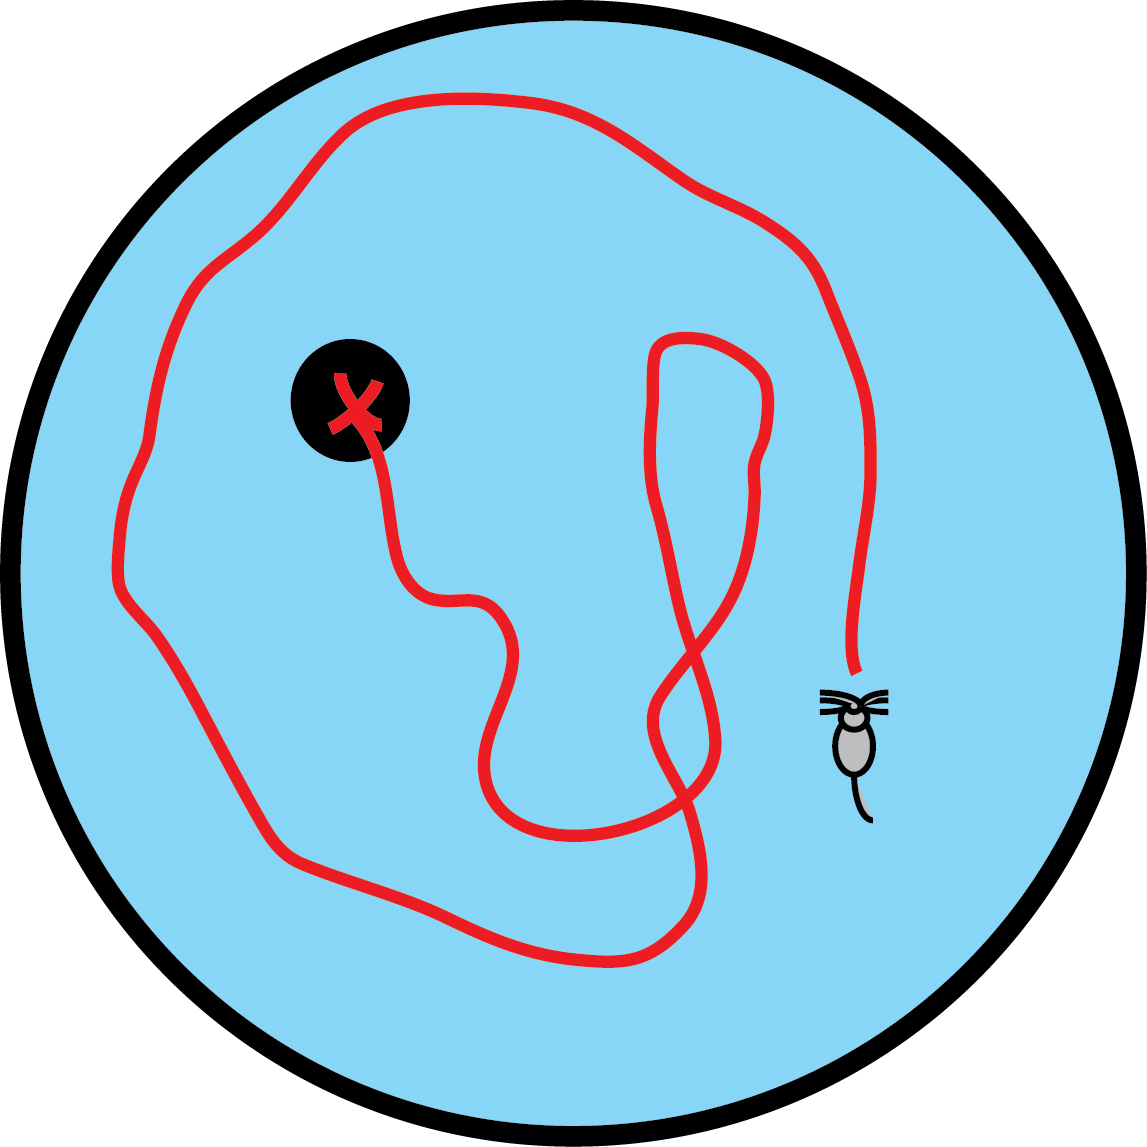
\includegraphics[width=0.4\textwidth]{figures/MWM}
		\end{figure}
	\end{multicols}
	\vspace{10mm}
	\begin{tiny}
		\begin{noindlist}
			\item $[1]$ D'Hooge, Rudi, and Peter P. De Deyn. ``Applications of the Morris water maze in the study of learning and memory.'' Brain research reviews 36.1 (2001): 60-90.
		\end{noindlist}
	\end{tiny}
\end{frame}

\begin{frame}{Data Analysis in the MWM}
	\begin{figure}[H]
		\centering
		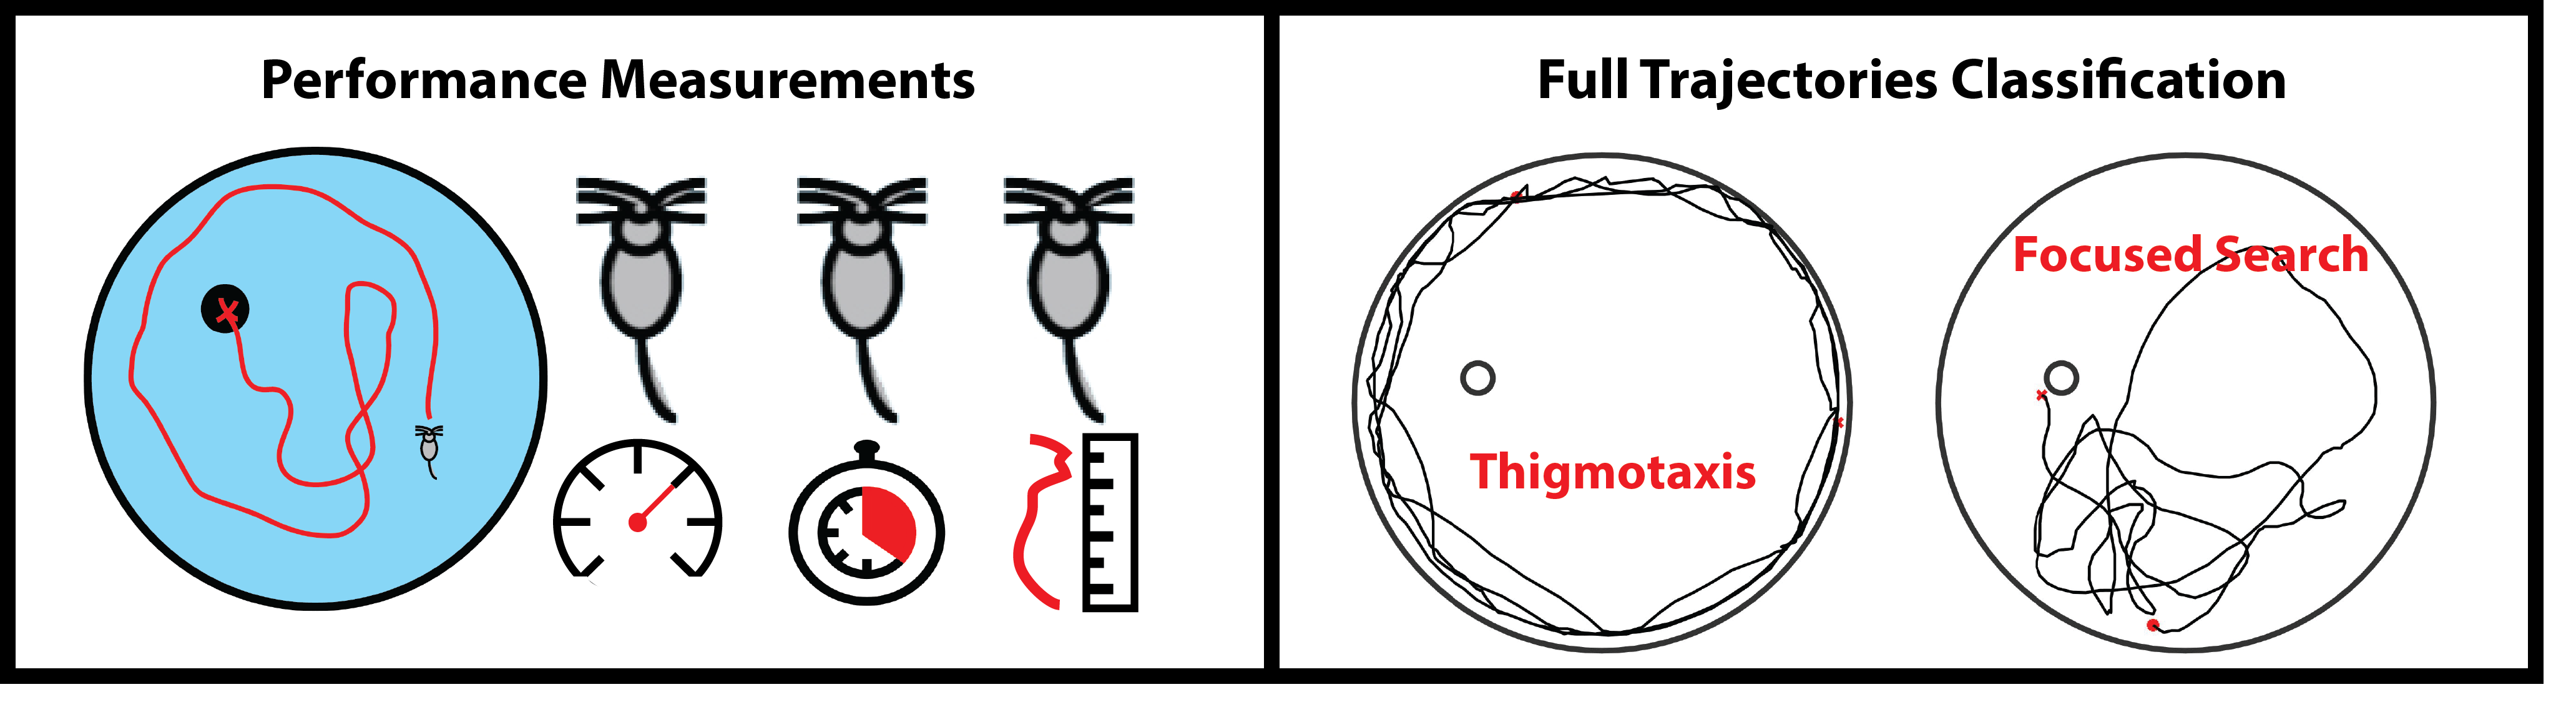
\includegraphics[width=\textwidth]{figures/nutshell-comb}
	\end{figure}
	\vspace{-2mm}
	\begin{itemize}
		\item<2-> \textbf{Performance measurements:} Insufficient to capture all the different animal behaviours that are present during the experiments [1].
		\vspace{3mm}
		\item<3-> \textbf{Full trajectories classification:} Animals employ several behaviours during each trial in order to find the platform and by assigning whole animal trajectories to single behavioural classes results in the loss of important information [2].		
	\end{itemize}
	\vspace{1.3mm}
	\begin{tiny}
		\begin{noindlist}
			\item<2-> $[1]$ Dalm, Sergiu, et al. ``Quantification of swim patterns in the Morris water maze.'' Behavior Research Methods, Instruments, \& Computers 32.1 (2000): 134-139.
			\item<3-> $[2]$ Gehring, Tiago V., et al. ``Detailed classification of swimming paths in the Morris Water Maze: multiple strategies within one trial.'' Scientific reports 5 (2015): 14562.
		\end{noindlist}
	\end{tiny}
\end{frame}

\begin{frame}{Data Analysis in the MWM}
	\begin{figure}[H]
		\centering
		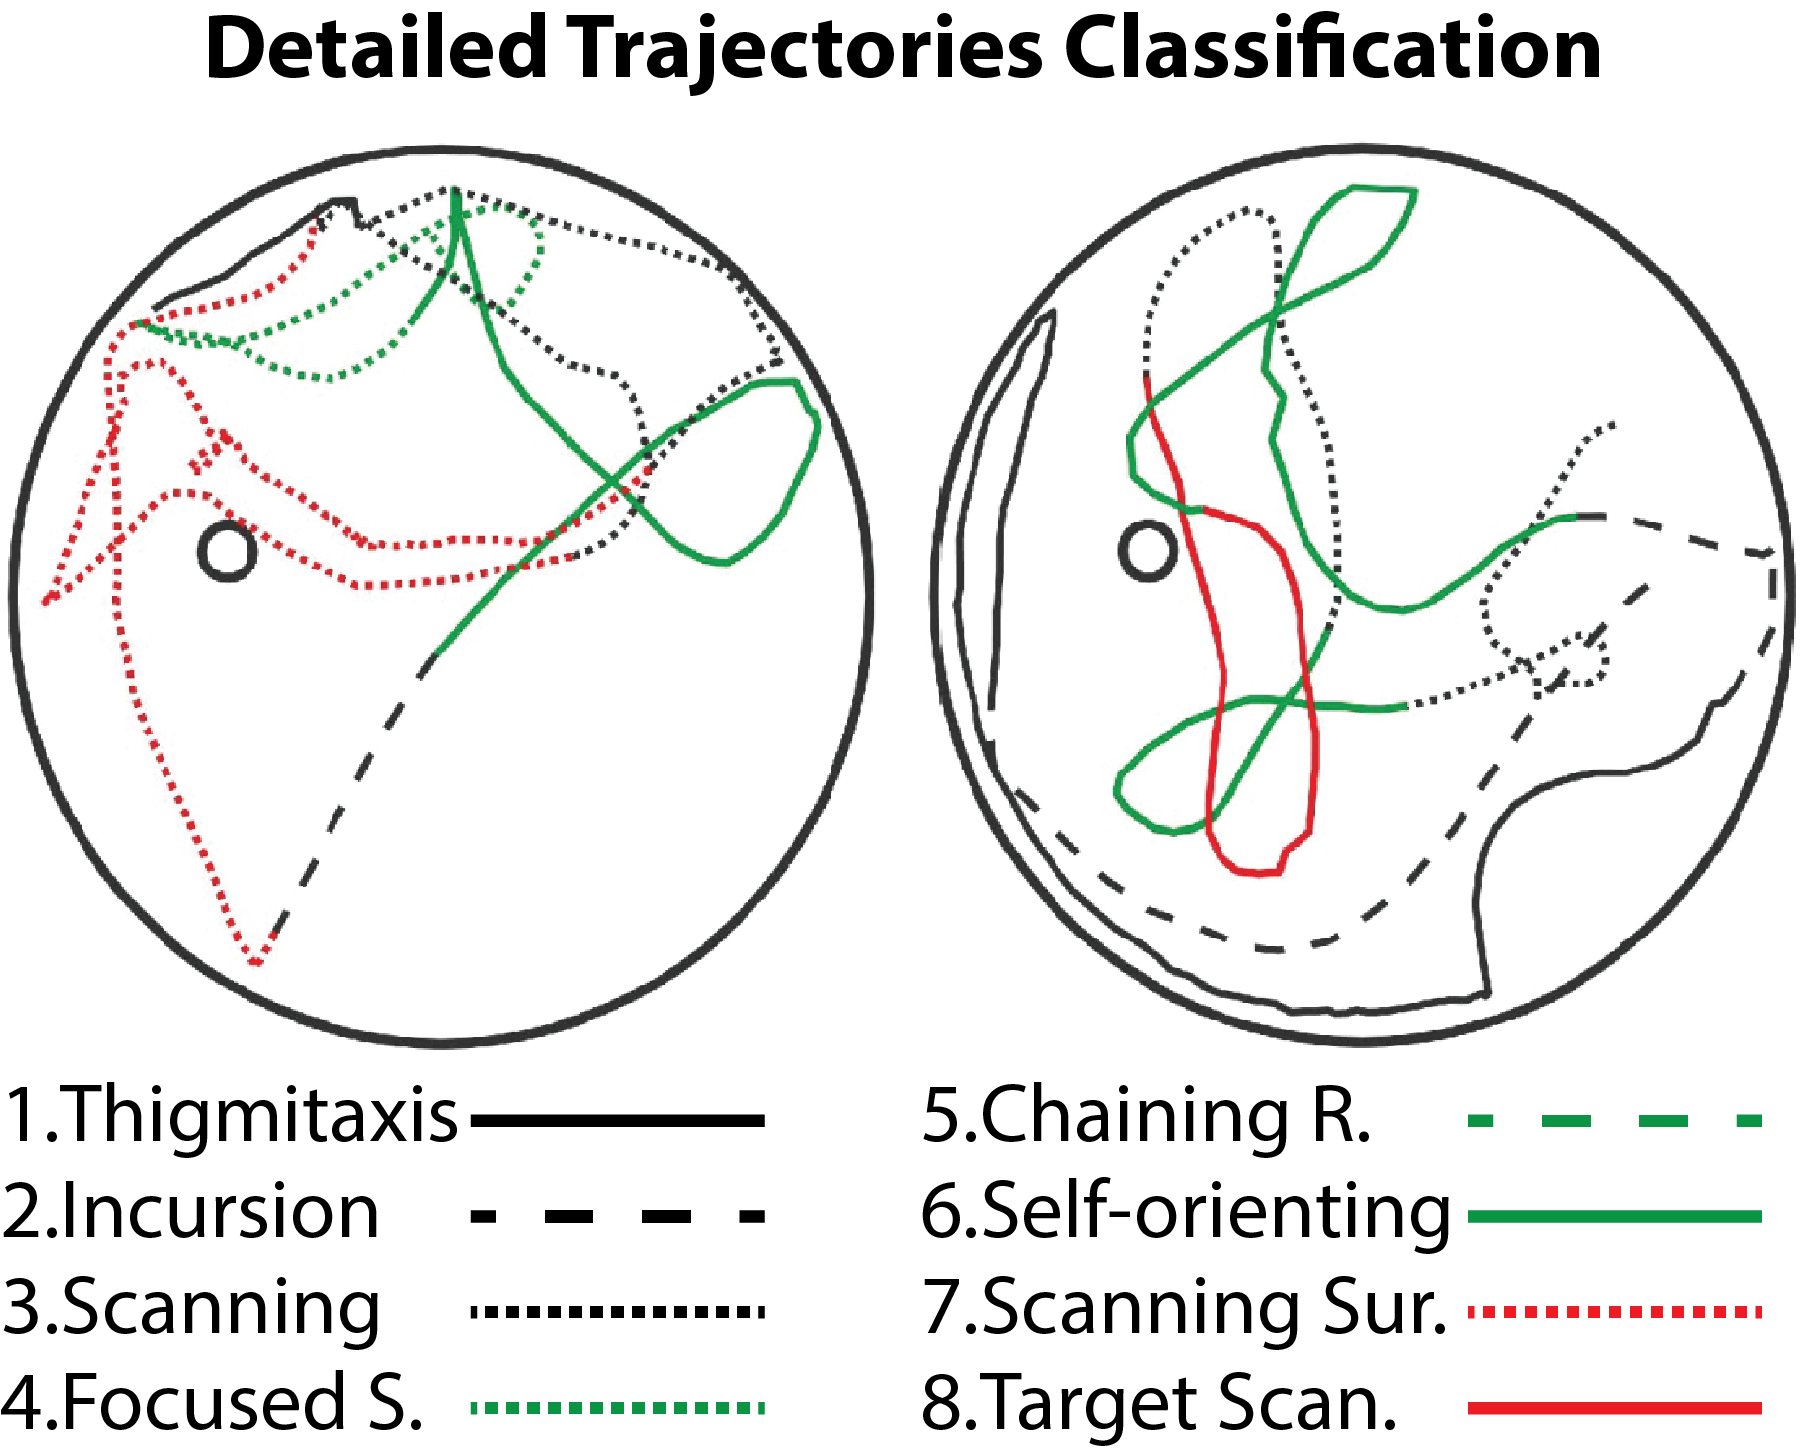
\includegraphics[width=0.65\textwidth]{figures/nutshell-c}
	\end{figure}
	\vspace{8mm}
	\begin{tiny}
		\begin{noindlist}
			\item $[1]$ Gehring, Tiago V., et al. ``Detailed classification of swimming paths in the Morris Water Maze: multiple strategies within one trial.'' Scientific reports 5 (2015): 14562.
		\end{noindlist}
	\end{tiny}
\end{frame}

\begin{frame}{Procedure of Gehring et al.}
	\begin{itemize}[leftmargin=-2mm]
		\setlength\itemsep{2.3em}
		\item[]<1-> 	
		\begin{figure}[H]
			\centering
			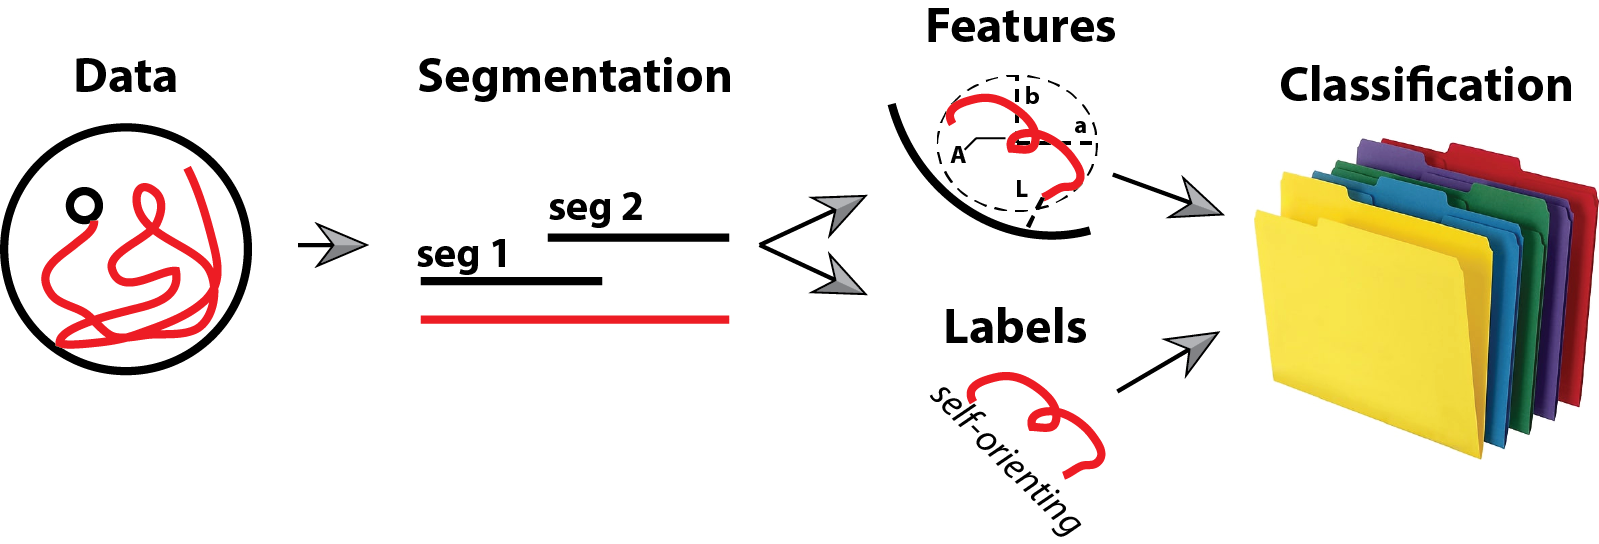
\includegraphics[width=0.8\textwidth]{figures/procedure1T}
		\end{figure}
		\item[]<2->
		\begin{figure}[H]
			\centering
			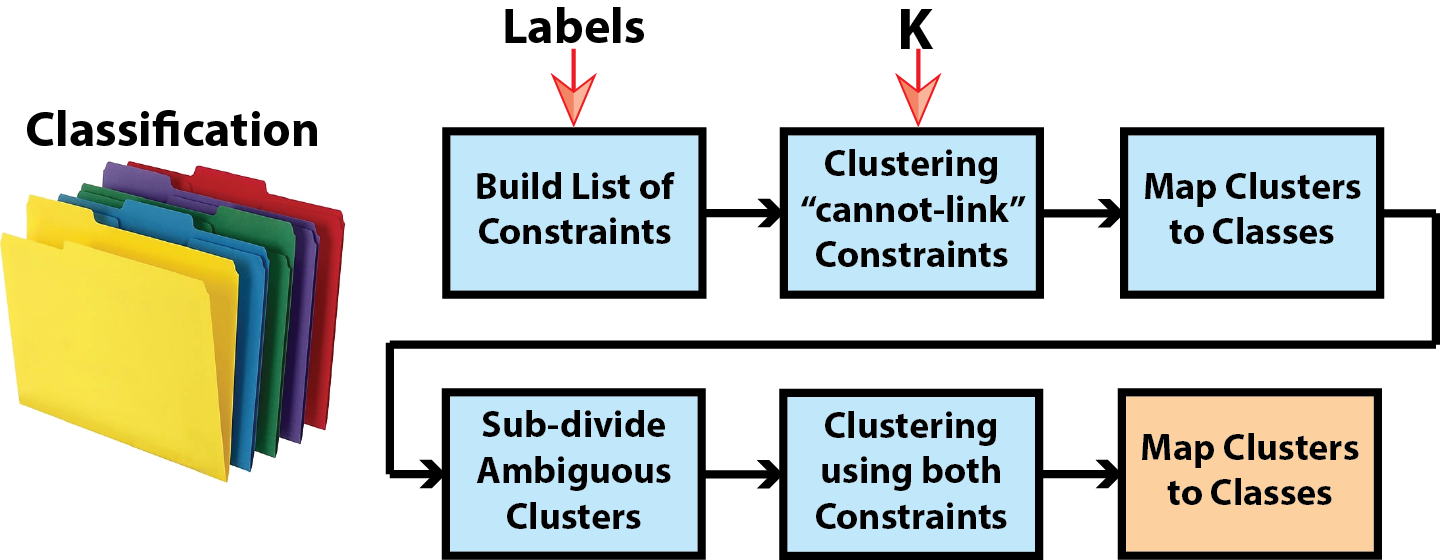
\includegraphics[width=0.8\textwidth]{figures/classificationT}
		\end{figure}
	\end{itemize}
\end{frame}

\begin{frame}{Procedure of Gehring et al.}
	\textbf{Mapping clusters to classes}	
	\vspace{3mm}		
	\begin{figure}[H]
		\centering
		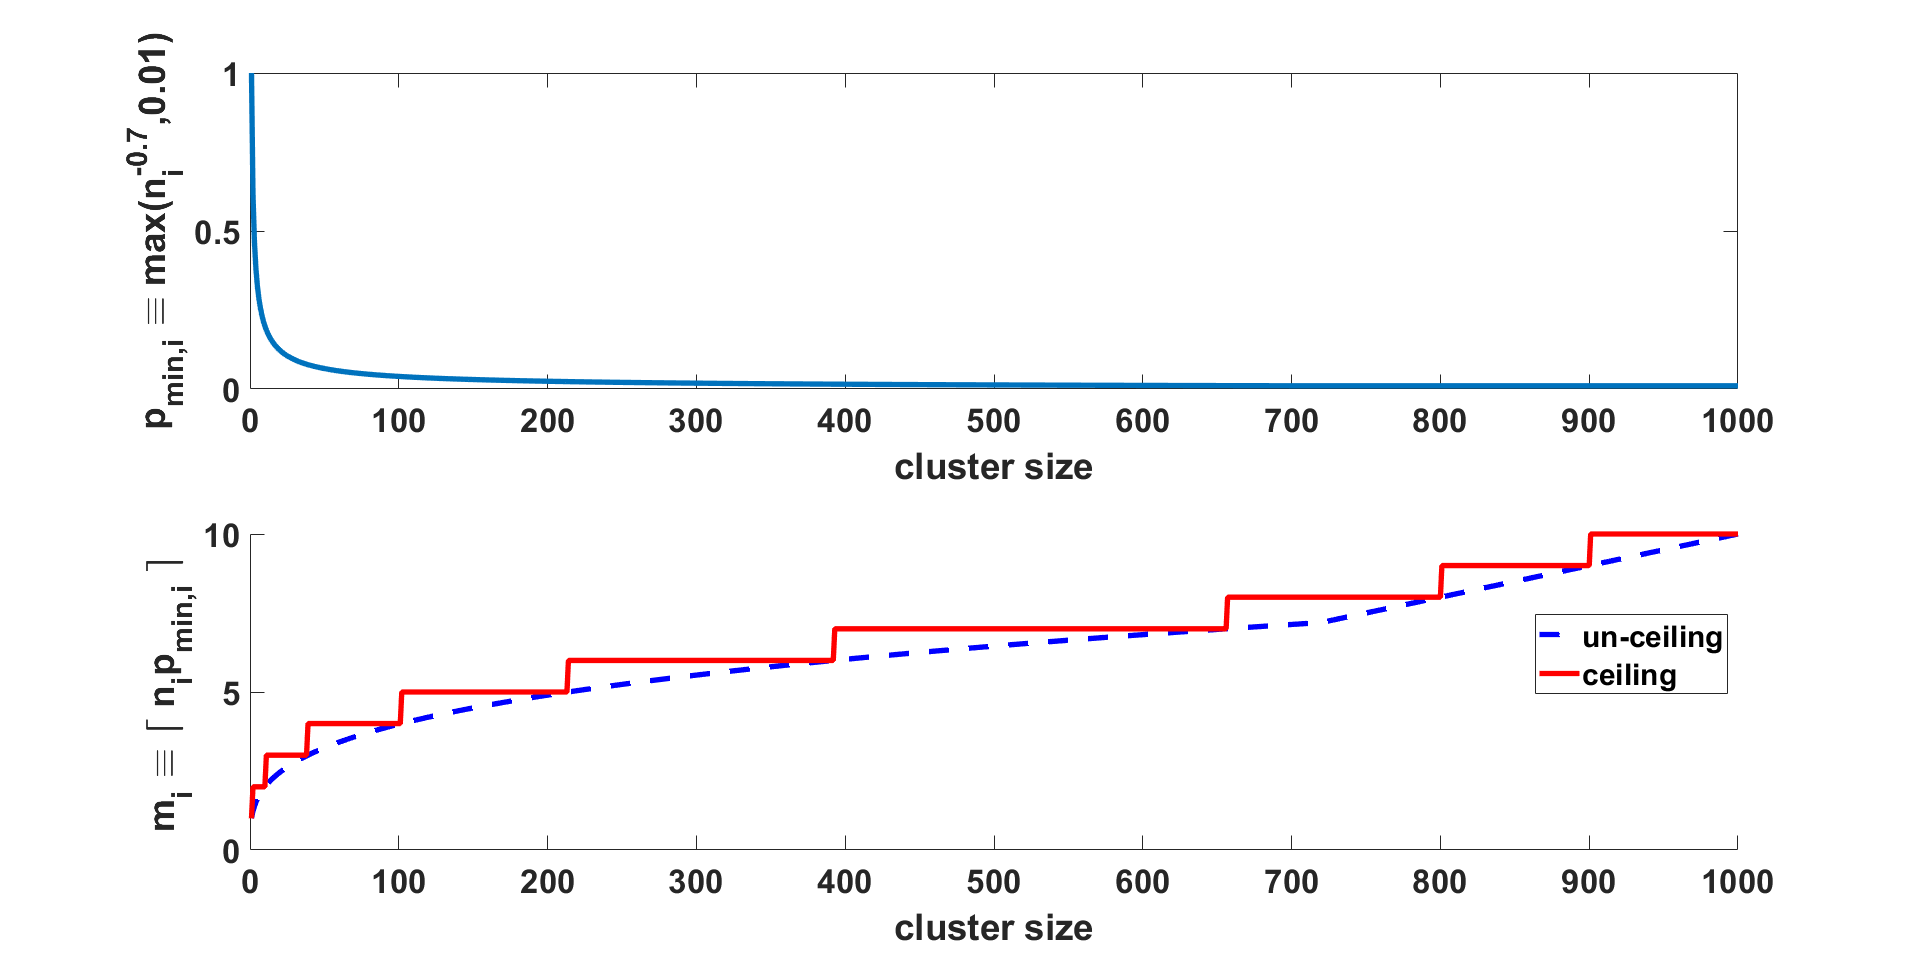
\includegraphics[width=\textwidth]{figures/clu2cla}
	\end{figure}
\end{frame}	
%Since the clustering algorithm generates clusters with a wide range of different sizes the minimum number of required labels of cluster i was made dependent on the cluster size; it was defined as mi=[ni*pmin,i] where ni is the cluster size, and pmin,i=max(ni^-g,pmin); g=0.7 and pmin=0.01 
%With the definition above a larger proportion of labelled data is required in the case of smaller clusters; for larger clusters this proportion gets smaller but is always at least 1%


\begin{frame}{Procedure of Gehring et al.}
	\textbf{Mapping segments back to the original trajectories}	
	\vspace{5mm}	
	\begin{itemize}[leftmargin=-2mm]
		\setlength\itemsep{2.3em}
		\item[]<1-> 	
		\begin{figure}[H]
			\centering
			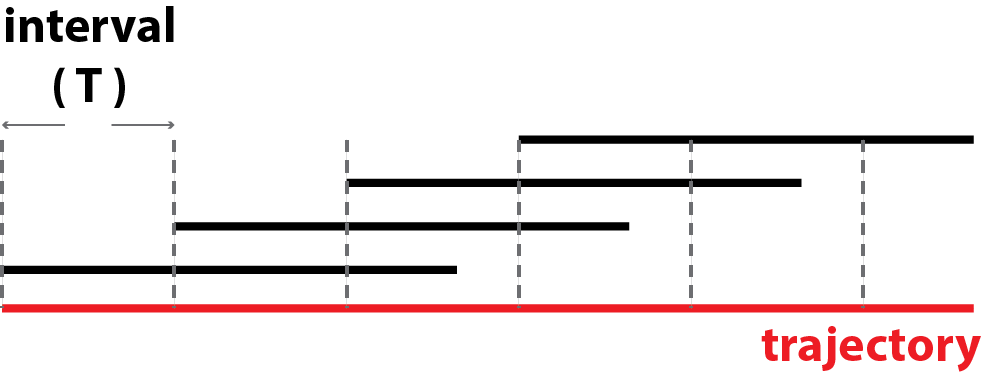
\includegraphics[width=0.6\textwidth]{figures/intervals1}
		\end{figure}
		\item[]<2-> 
		\begin{figure}[H]
			\centering
			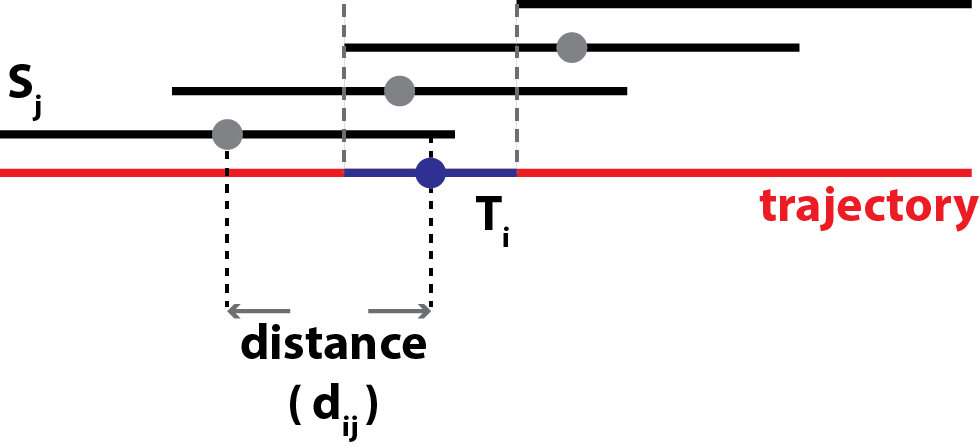
\includegraphics[width=0.6\textwidth]{figures/intervals2}
		\end{figure}
	\end{itemize}
\end{frame}	
\begin{frame}{Procedure of Gehring et al.}
	\textbf{Mapping segments back to the original trajectories}	
	\vspace{6mm}	
	\begin{itemize}[leftmargin=-2mm]
		\setlength\itemsep{2.3em}
		\item[]<1-> 	
		\begin{figure}[H]
			\centering
			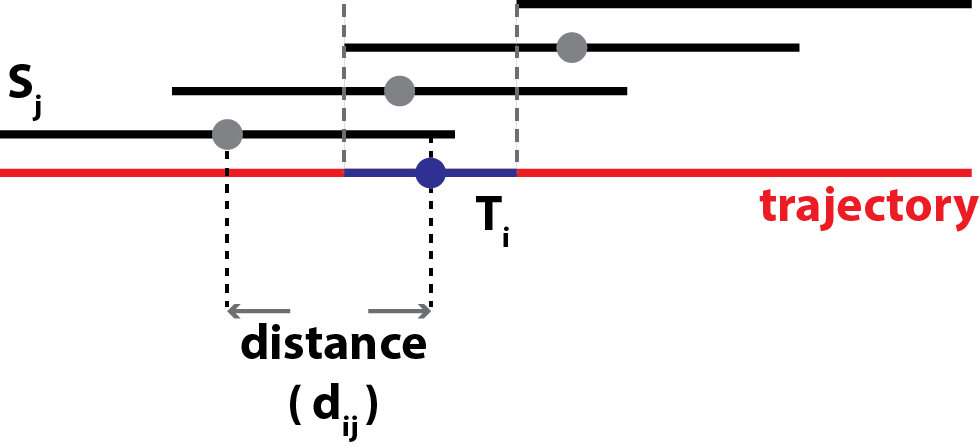
\includegraphics[width=0.6\textwidth]{figures/intervals2}
		\end{figure}
		\item[]<1-> 
		\begin{large}	
			\begin{equation*}
				C_{T_i} \equiv arg_{c_k}max\sum_{\binom{S_j \in c_k}{T_i\cap S_j\neq\varnothing}} w_k \cdot e^{-\frac{d_{ij}^2}{2 \cdot \sigma^2}},
				\textit{\invisible{xxxxx}}\sigma = 4, \textit{\invisible{x}} w_k = \frac{L_{max}^{cont}}{L_{max,k}}
			\end{equation*}	
		\end{large}
	\end{itemize}
\end{frame}	

\begin{frame}{Procedure of Gehring et al.}
	\textbf{How to find K?}	
	\vspace{3mm}
	\begin{itemize}[leftmargin=-2mm]
		\setlength{\itemindent}{0em}
		\item[]<1->
		\begin{figure}[H]
			\centering
			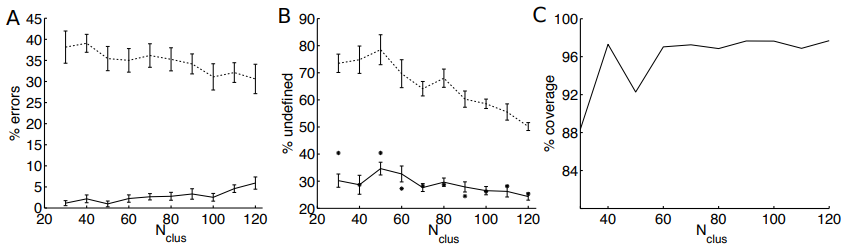
\includegraphics[width=\textwidth]{figures/kvalidation}
		\end{figure}
		\item[]<2->	
		\begin{figure}[H]
			\centering
			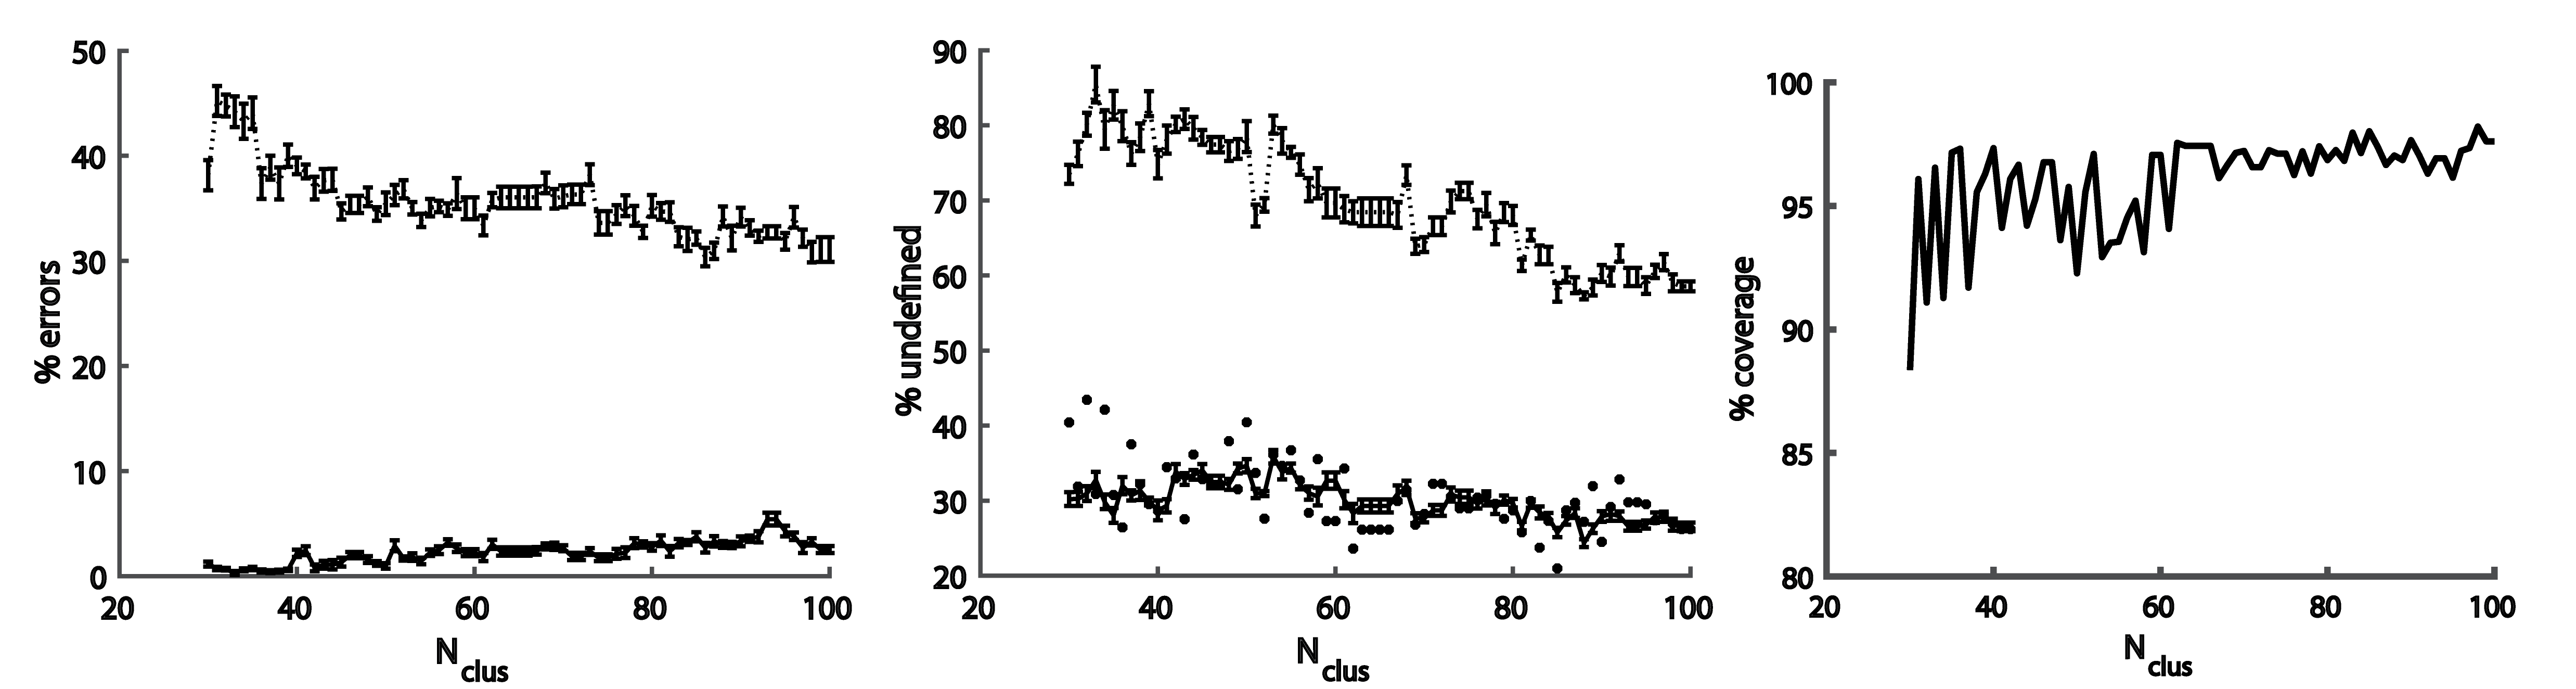
\includegraphics[width=\textwidth]{figures/kvalidationC}
		\end{figure}
	\end{itemize}
\end{frame}

\begin{frame}{Procedure of Gehring et al.}
	\begin{itemize}[label={\MyShadow{$\bullet$}{blue!80}}]
		\item Segmentation tuning.
		\vspace{3mm}
		\item Labelling.
		\vspace{3mm}
		\item Classification tuning.	
		\vspace{3mm}
		\item Final conclusions are based on different segmentation tunings combined together.		
	\end{itemize}
\end{frame}


\begin{frame}{Procedure of Vouros et al.}
	\textbf{How to find K?}
	\vspace{7mm}
	\begin{figure}[H]
		\centering
		
\includegraphics[width=0.7\textwidth]{figures/maths}
	\end{figure}
	\vspace{20mm}
\end{frame}

\begin{frame}{Procedure of Vouros et al.}
	\textbf{Classification boosting with majority voting}
	\vspace{1mm}
	\begin{figure}[H]
		\centering
		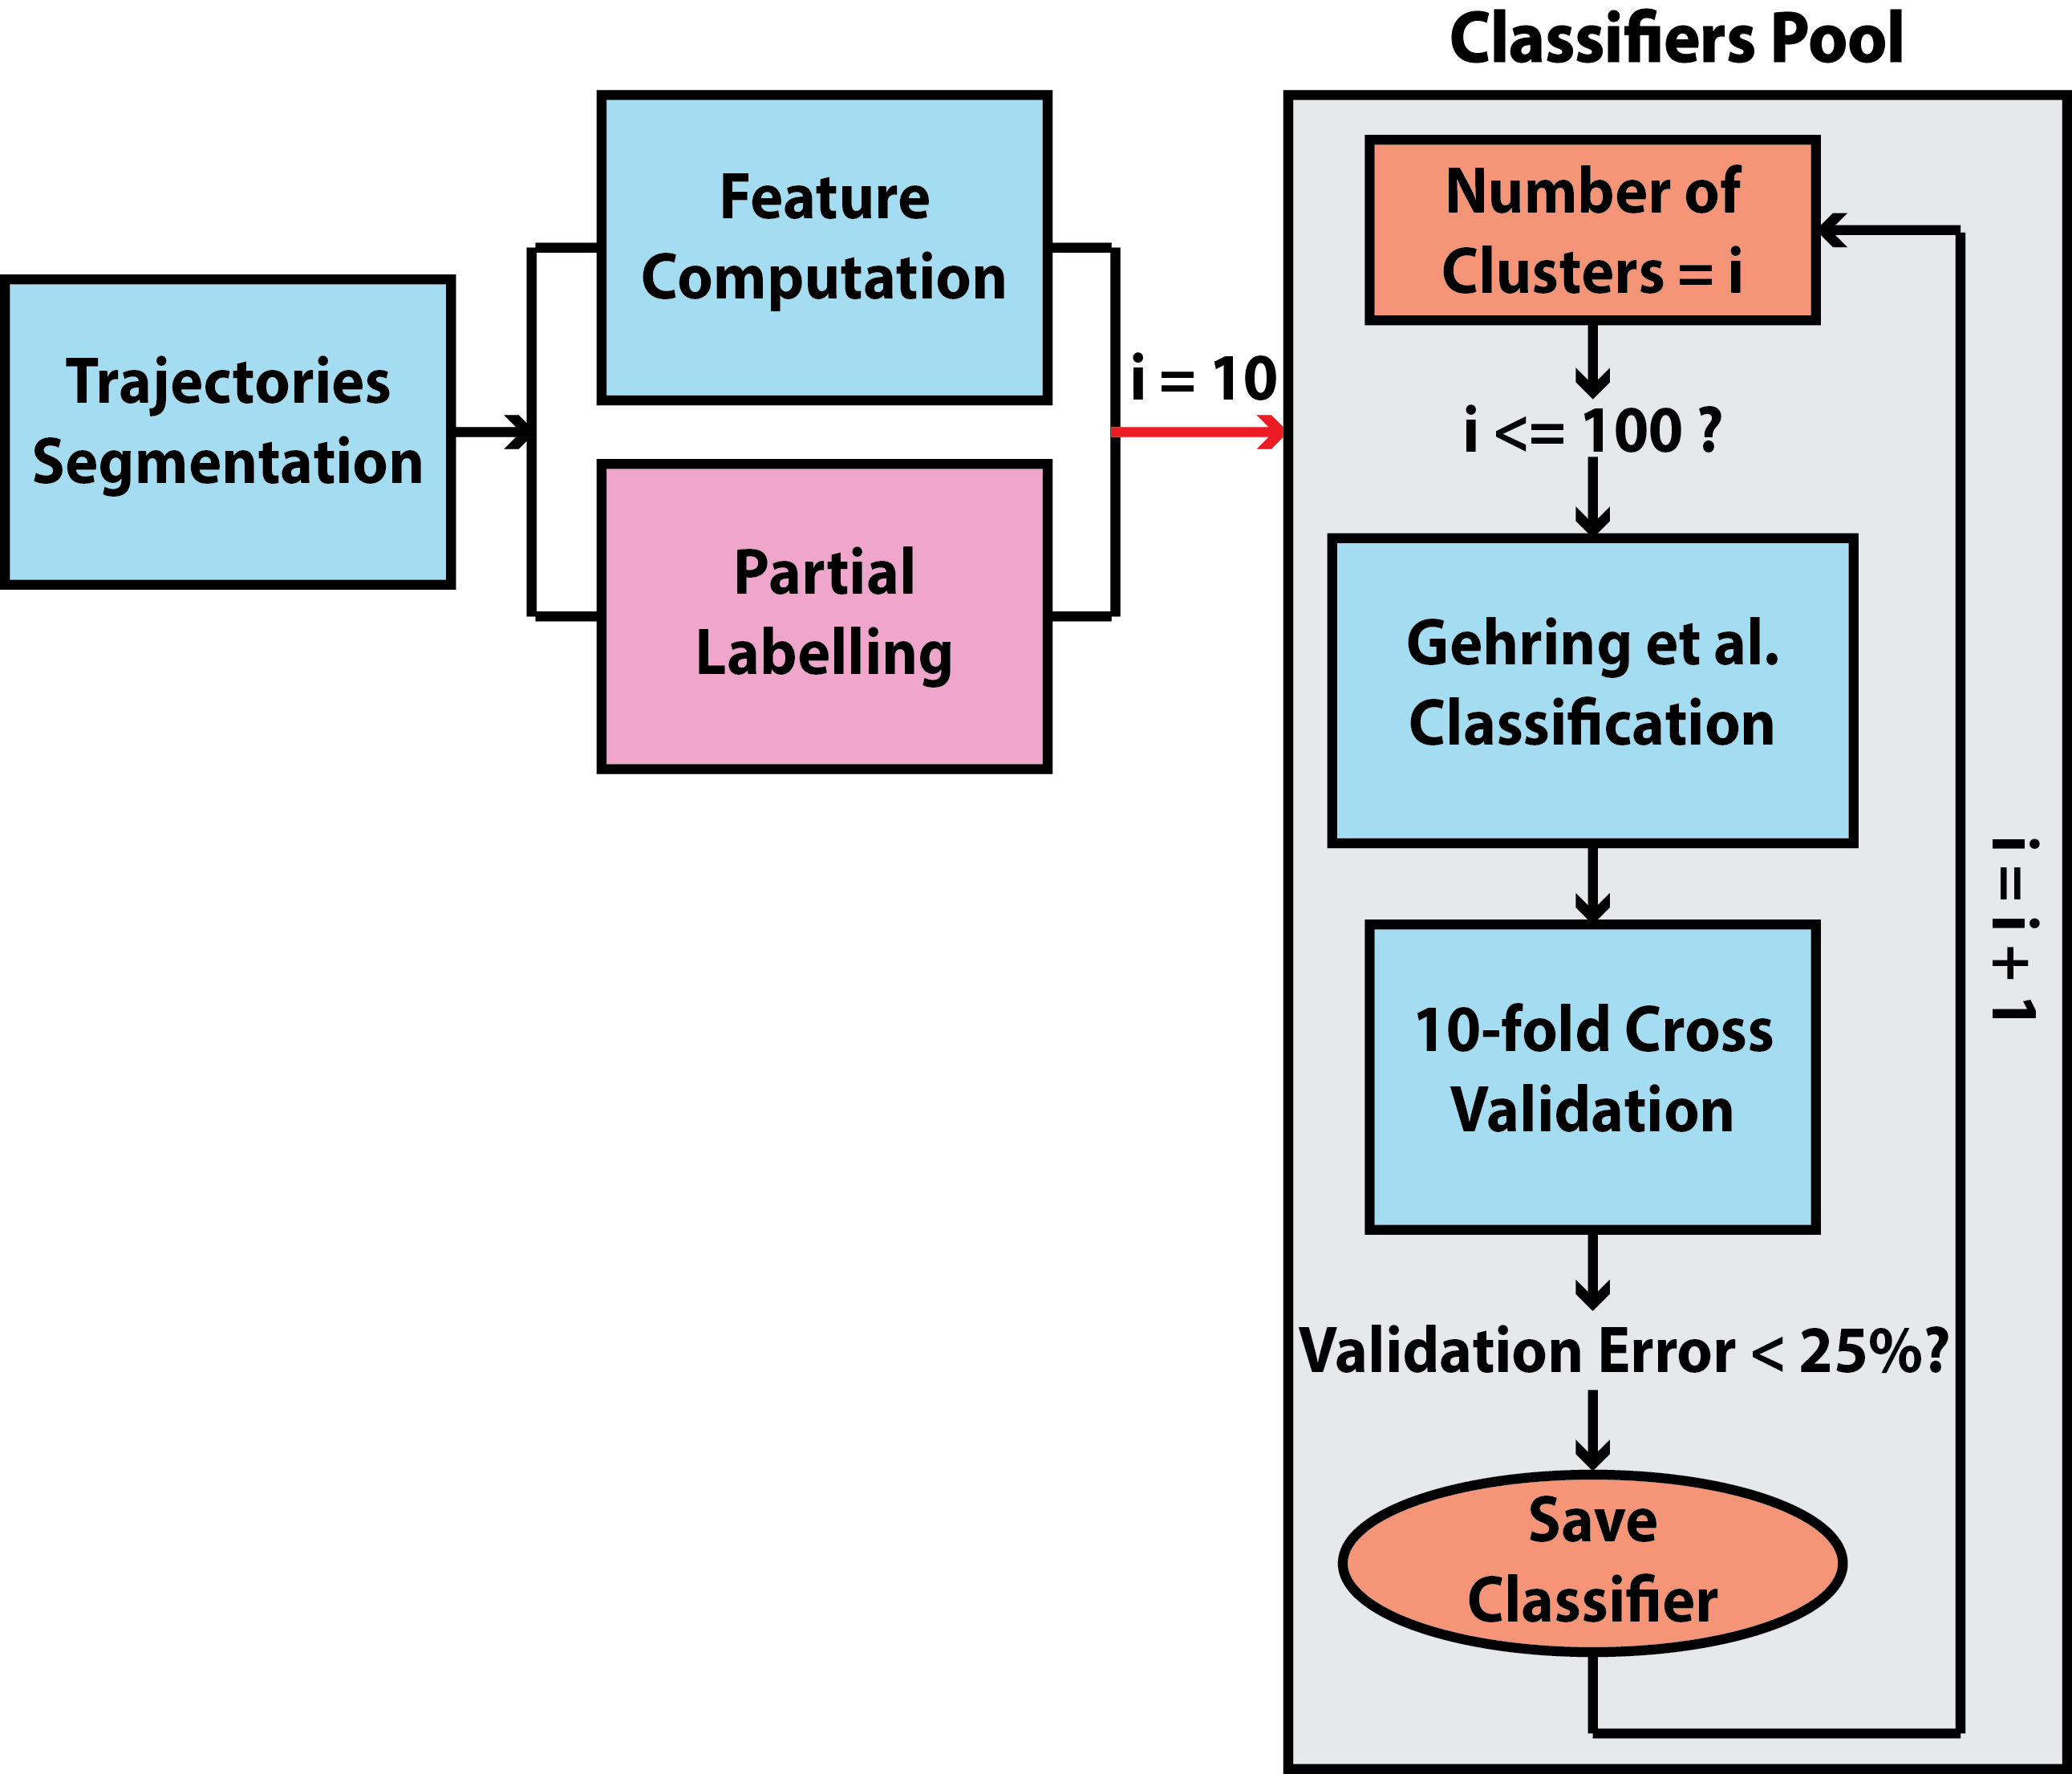
\includegraphics[width=0.7\textwidth]{figures/boosting1}
	\end{figure}
\end{frame}
\begin{frame}{Procedure of Vouros et al.}
	\textbf{Classification boosting with majority voting}
	\vspace{1mm}
	\begin{figure}[H]
		\centering
		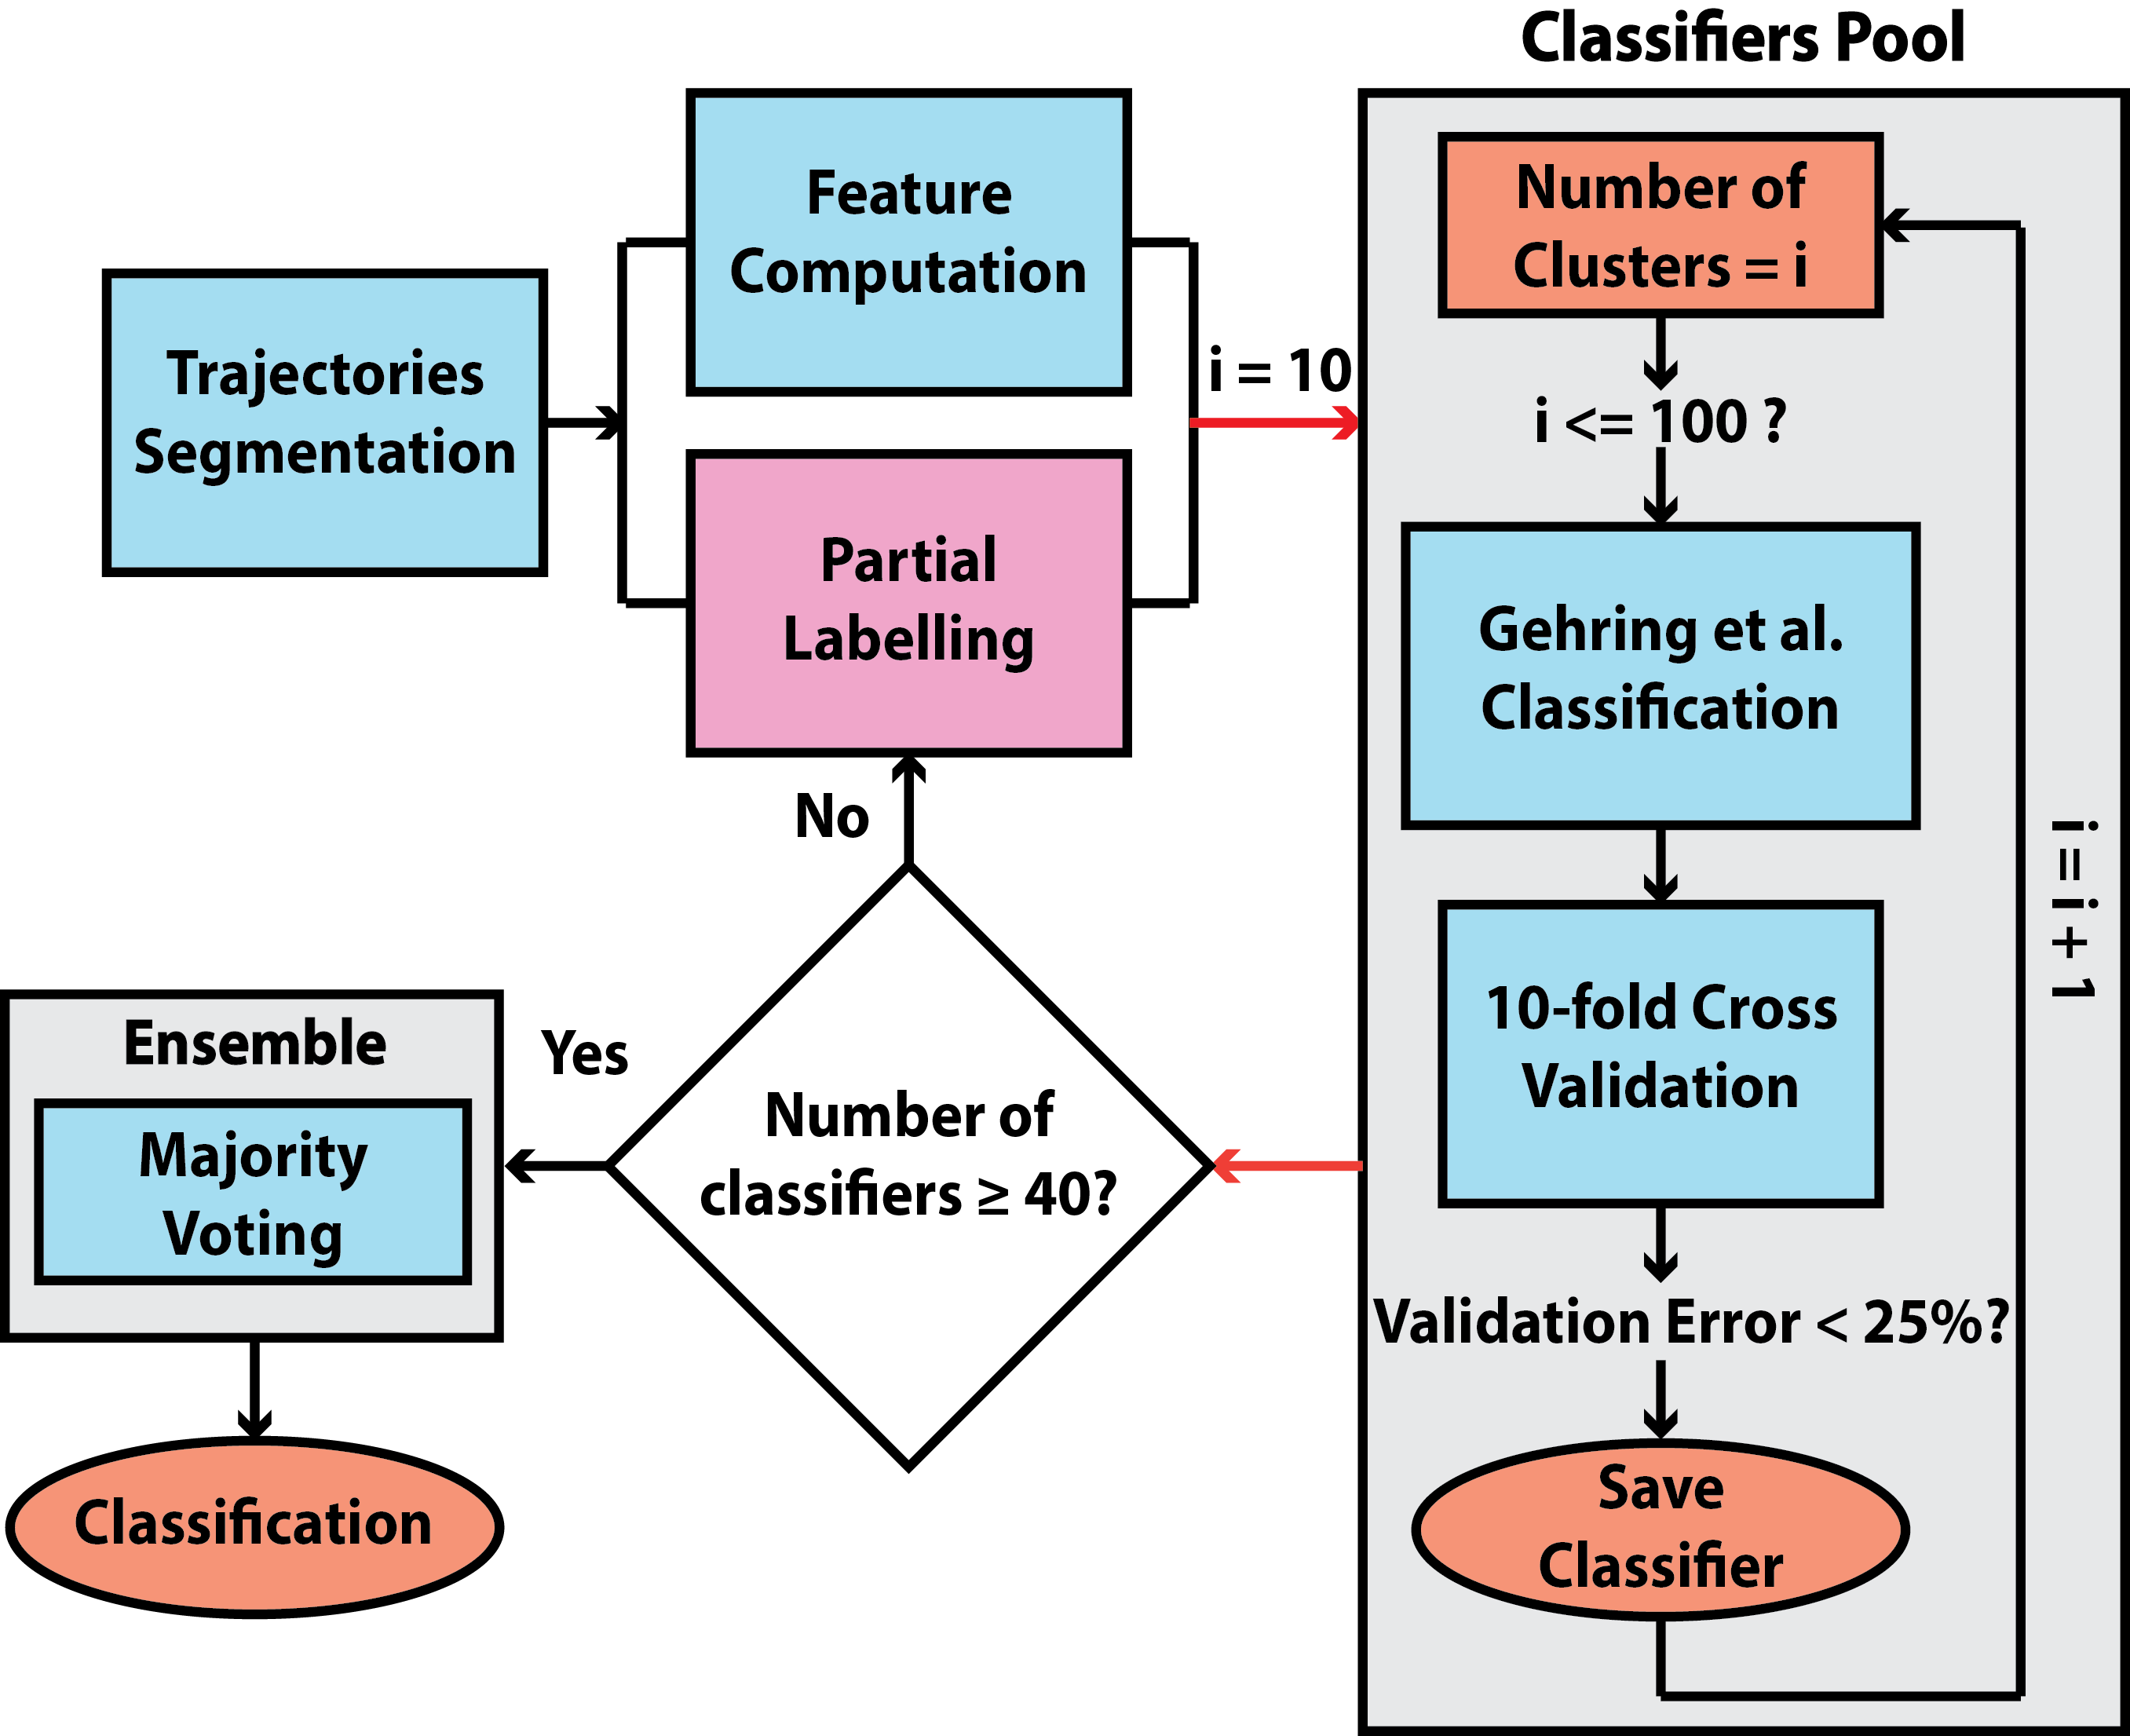
\includegraphics[width=0.7\textwidth]{figures/boosting2}
	\end{figure}
\end{frame}

\begin{frame}{Procedure of Vouros et al.}
	\textbf{Mapping segments back to the original trajectories:}\\ 
	\textit{segmentation independent, $T$ and $\sigma$ proportional to $R$}
	\vspace{5mm}	
	\begin{itemize}[leftmargin=-2mm]
		\setlength\itemsep{2.3em}
		\item[]<1-> 	
		\begin{figure}[H]
			\centering
			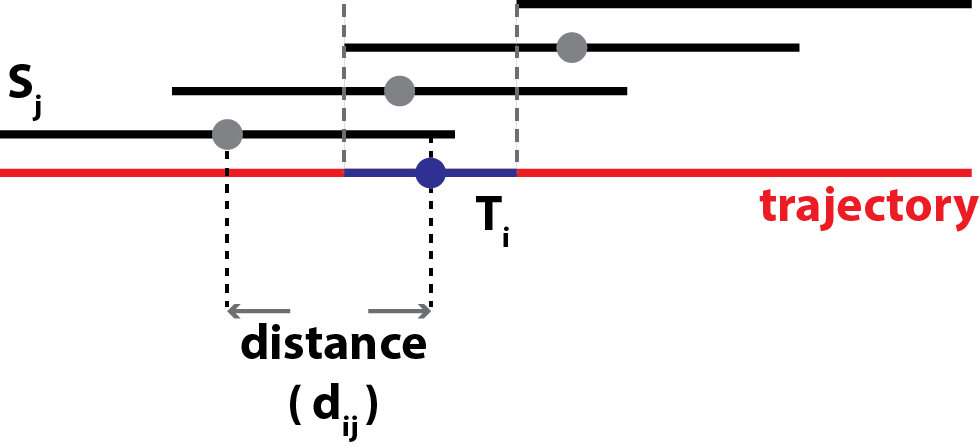
\includegraphics[width=0.6\textwidth]{figures/intervals2}
		\end{figure}
		\item[]<1-> 
		\begin{large}	
			\begin{equation*}
			C_{T_i} \equiv arg_{c_k}max\sum_{\binom{S_j \in c_k}{T_i\cap S_j\neq\varnothing}} w_k \cdot e^{-\frac{d_{ij}^2}{2 \cdot \sigma^2}},
			\textit{\invisible{xxxxx}}w_k = \frac{1}{P(c_k)}
			\end{equation*}	
		\end{large}
	\end{itemize}
\end{frame}

\begin{frame}{Procedure of Vouros et al.}
	\textbf{Validation and Confidence}
	\vspace{5mm}
	\begin{figure}[H]
		\centering
		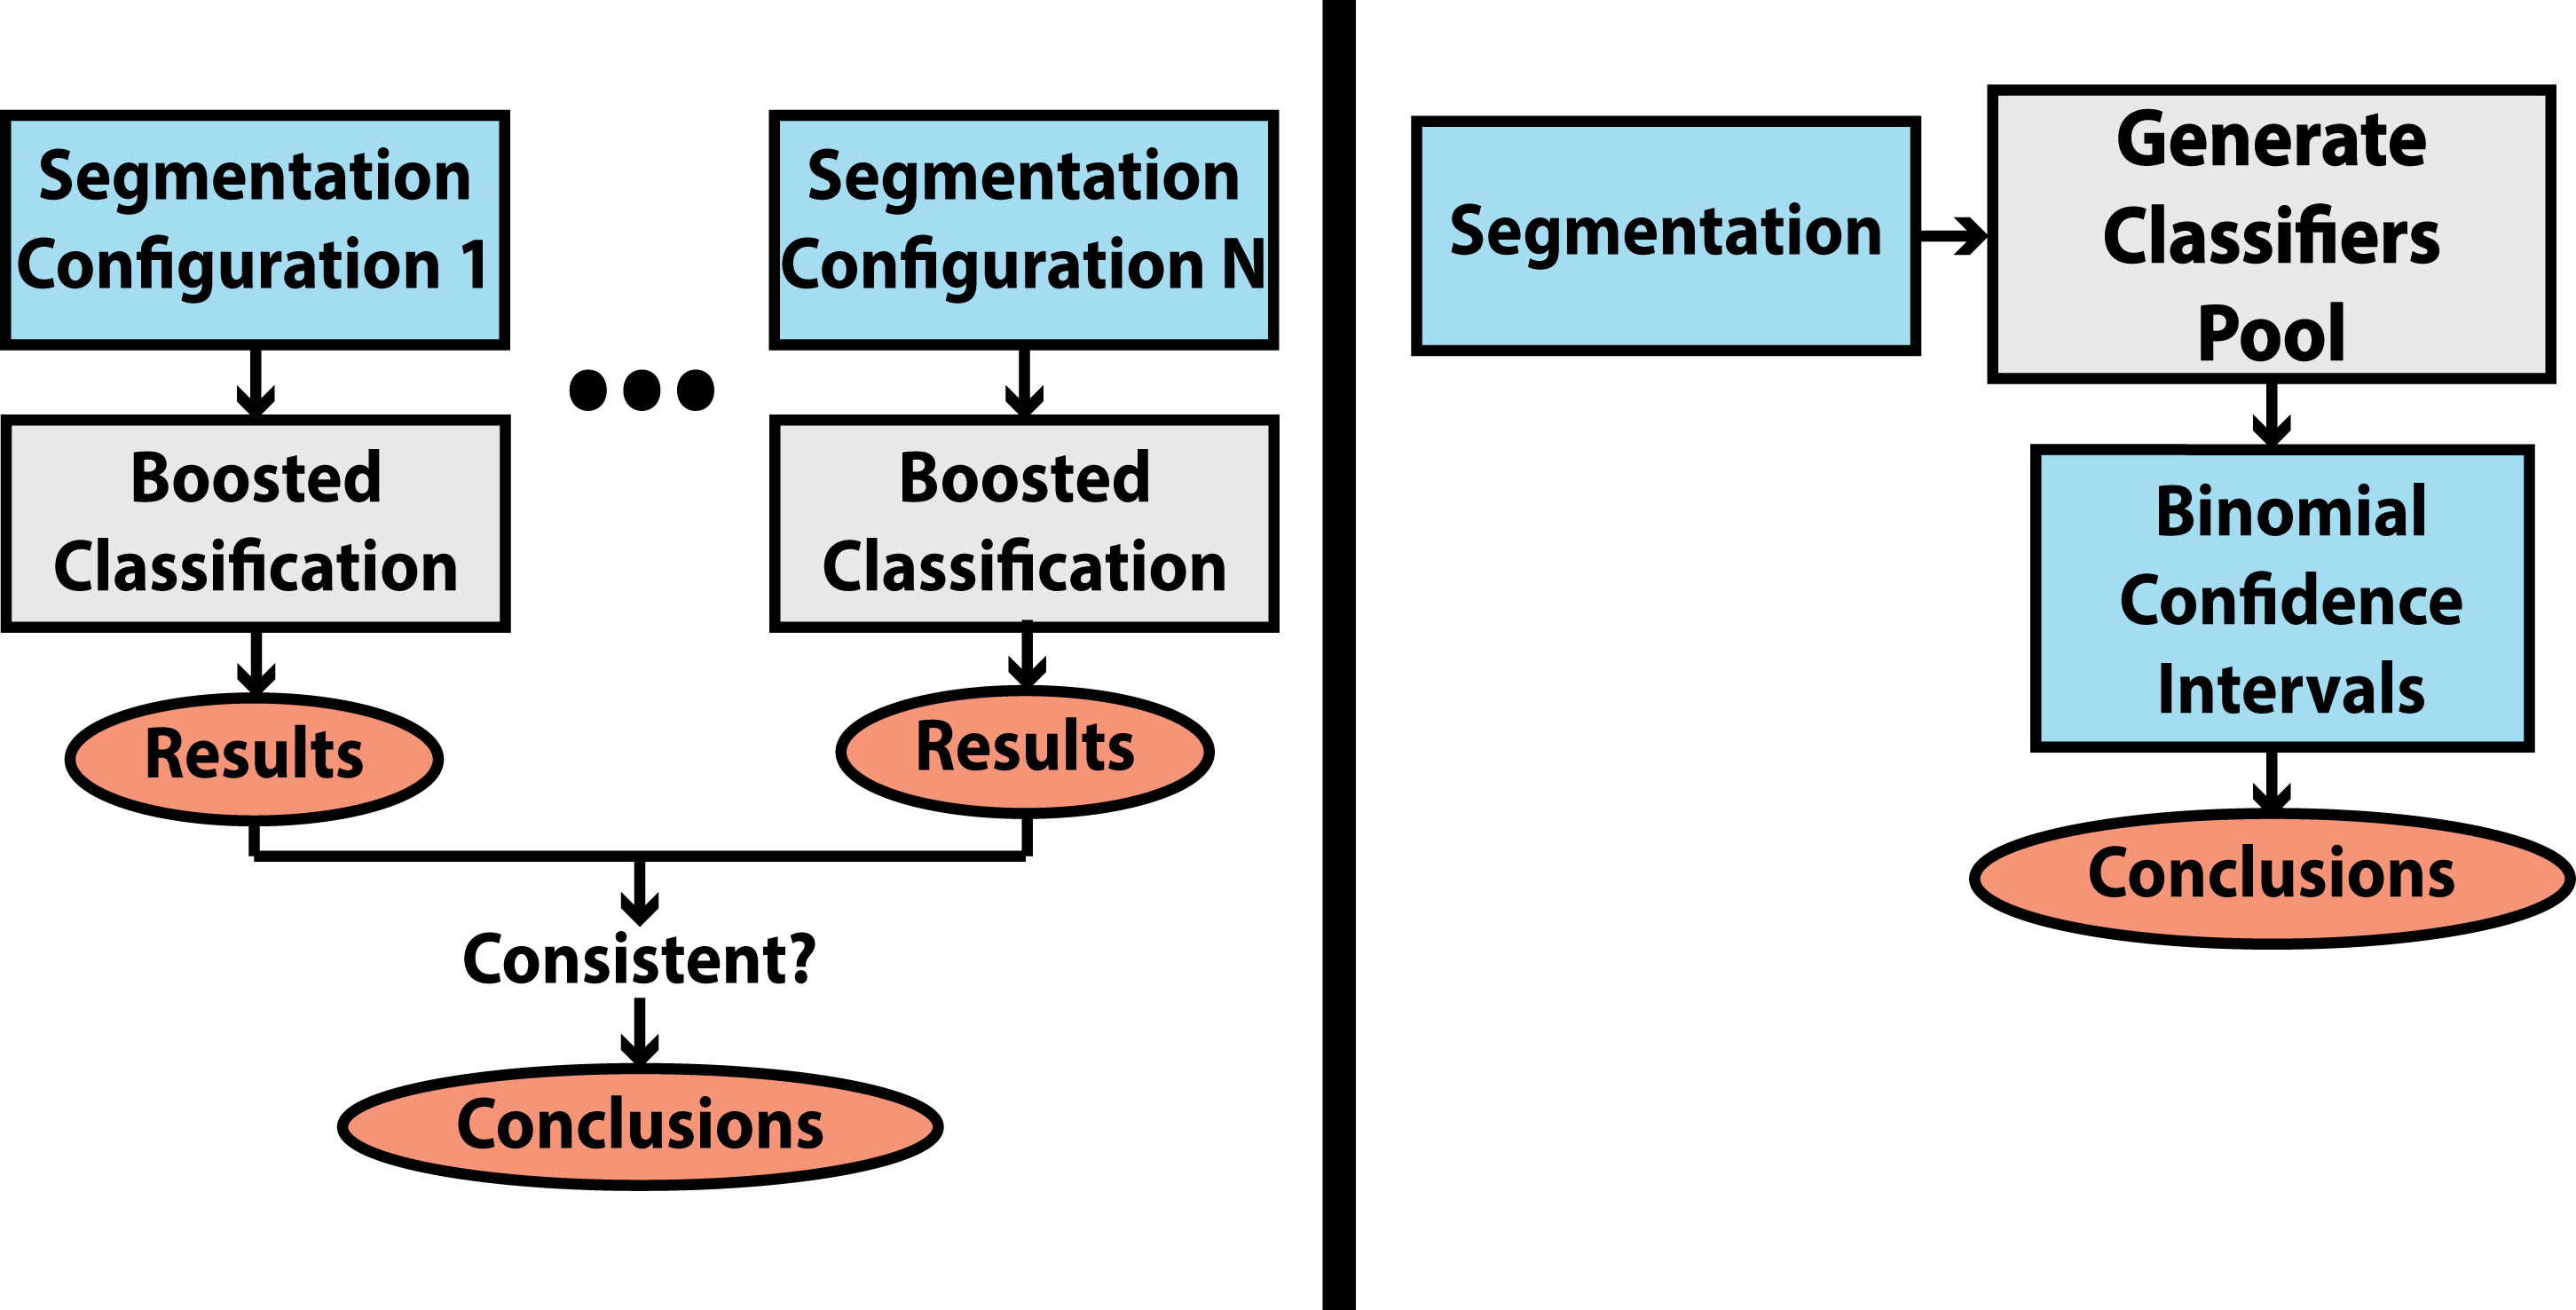
\includegraphics[width=0.9\textwidth]{figures/testing}
	\end{figure}
	\vspace{15mm}
\end{frame}

\begin{frame}{Results}
	\begin{figure}[H]
		\centering
		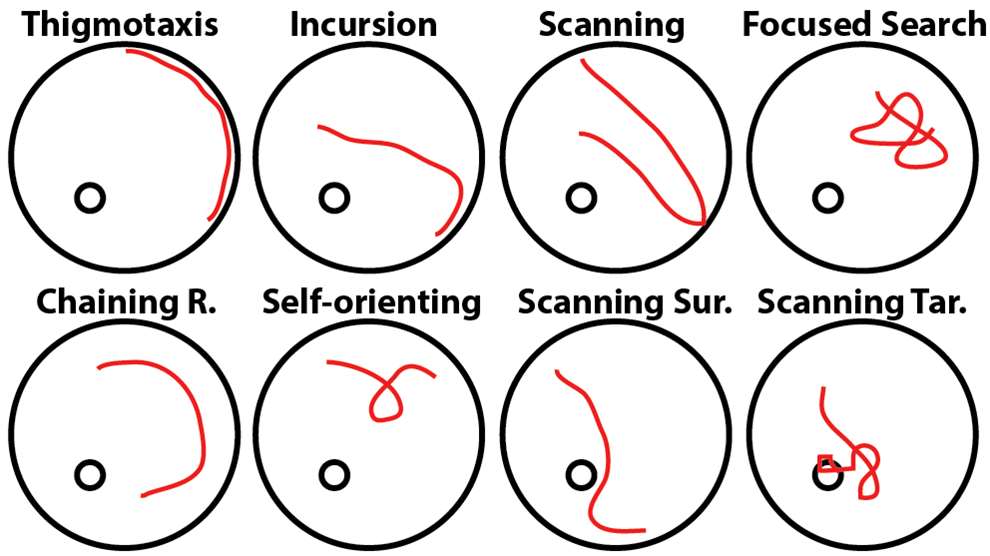
\includegraphics[width=0.8\textwidth]{figures/res1}
	\end{figure}
	\vspace{15mm}
\end{frame}

\begin{frame}{Results: EPFL - Stress vs Control Groups}
	\begin{figure}[H]
		\centering
		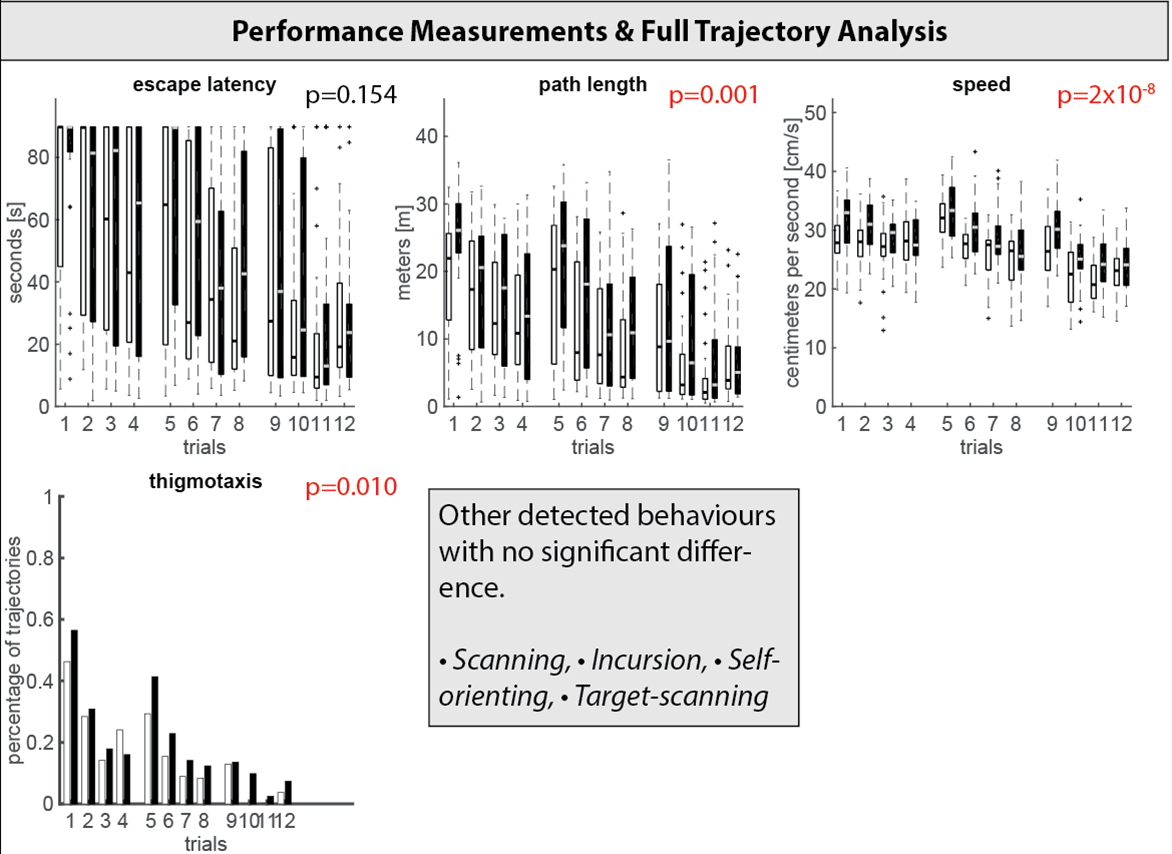
\includegraphics[width=0.9\textwidth]{figures/res2}
	\end{figure}
	\vspace{15mm}
\end{frame}

\begin{frame}{Results: EPFL - Stress vs Control Groups}
	\begin{figure}[H]
		\centering
		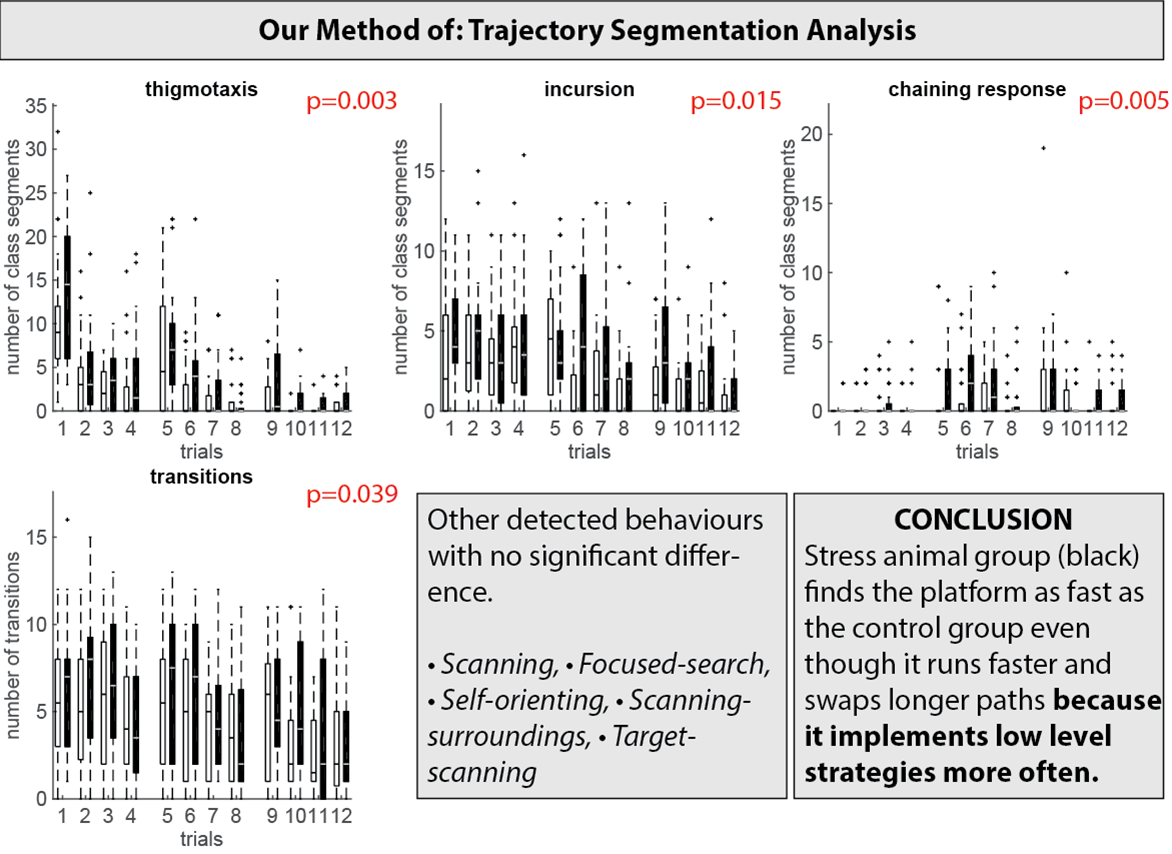
\includegraphics[width=0.9\textwidth]{figures/res3}
	\end{figure}
	\vspace{15mm}
\end{frame}

\begin{frame}{Results: EPFL - Stress vs Control Groups}
	\begin{figure}[H]
		\centering
		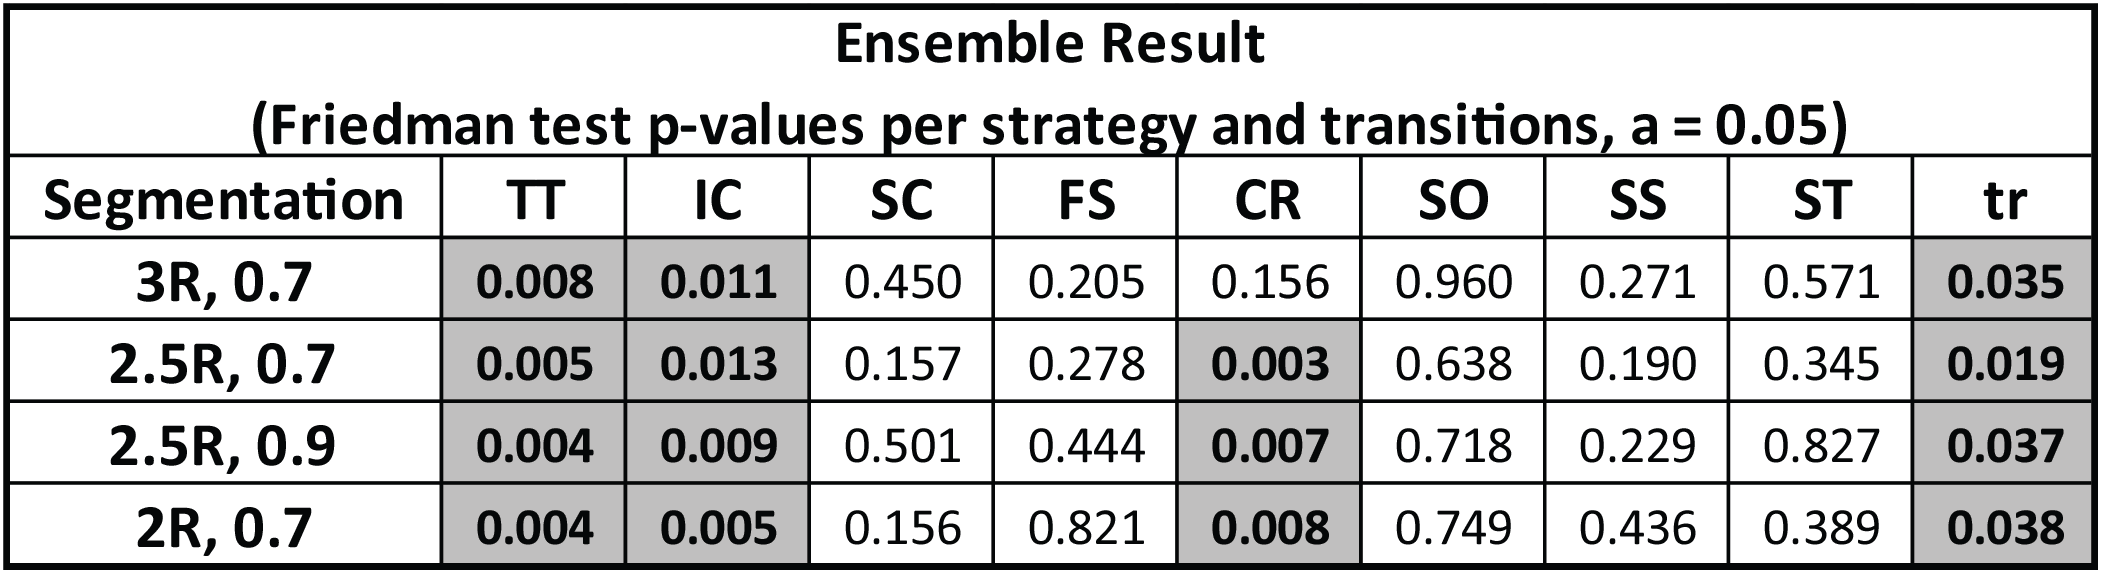
\includegraphics[width=\textwidth]{figures/res5}
	\end{figure}
	\vspace{15mm}
\end{frame}

\begin{frame}{Results: EPFL - Stress vs Control Groups}
	\begin{figure}[H]
		\centering
		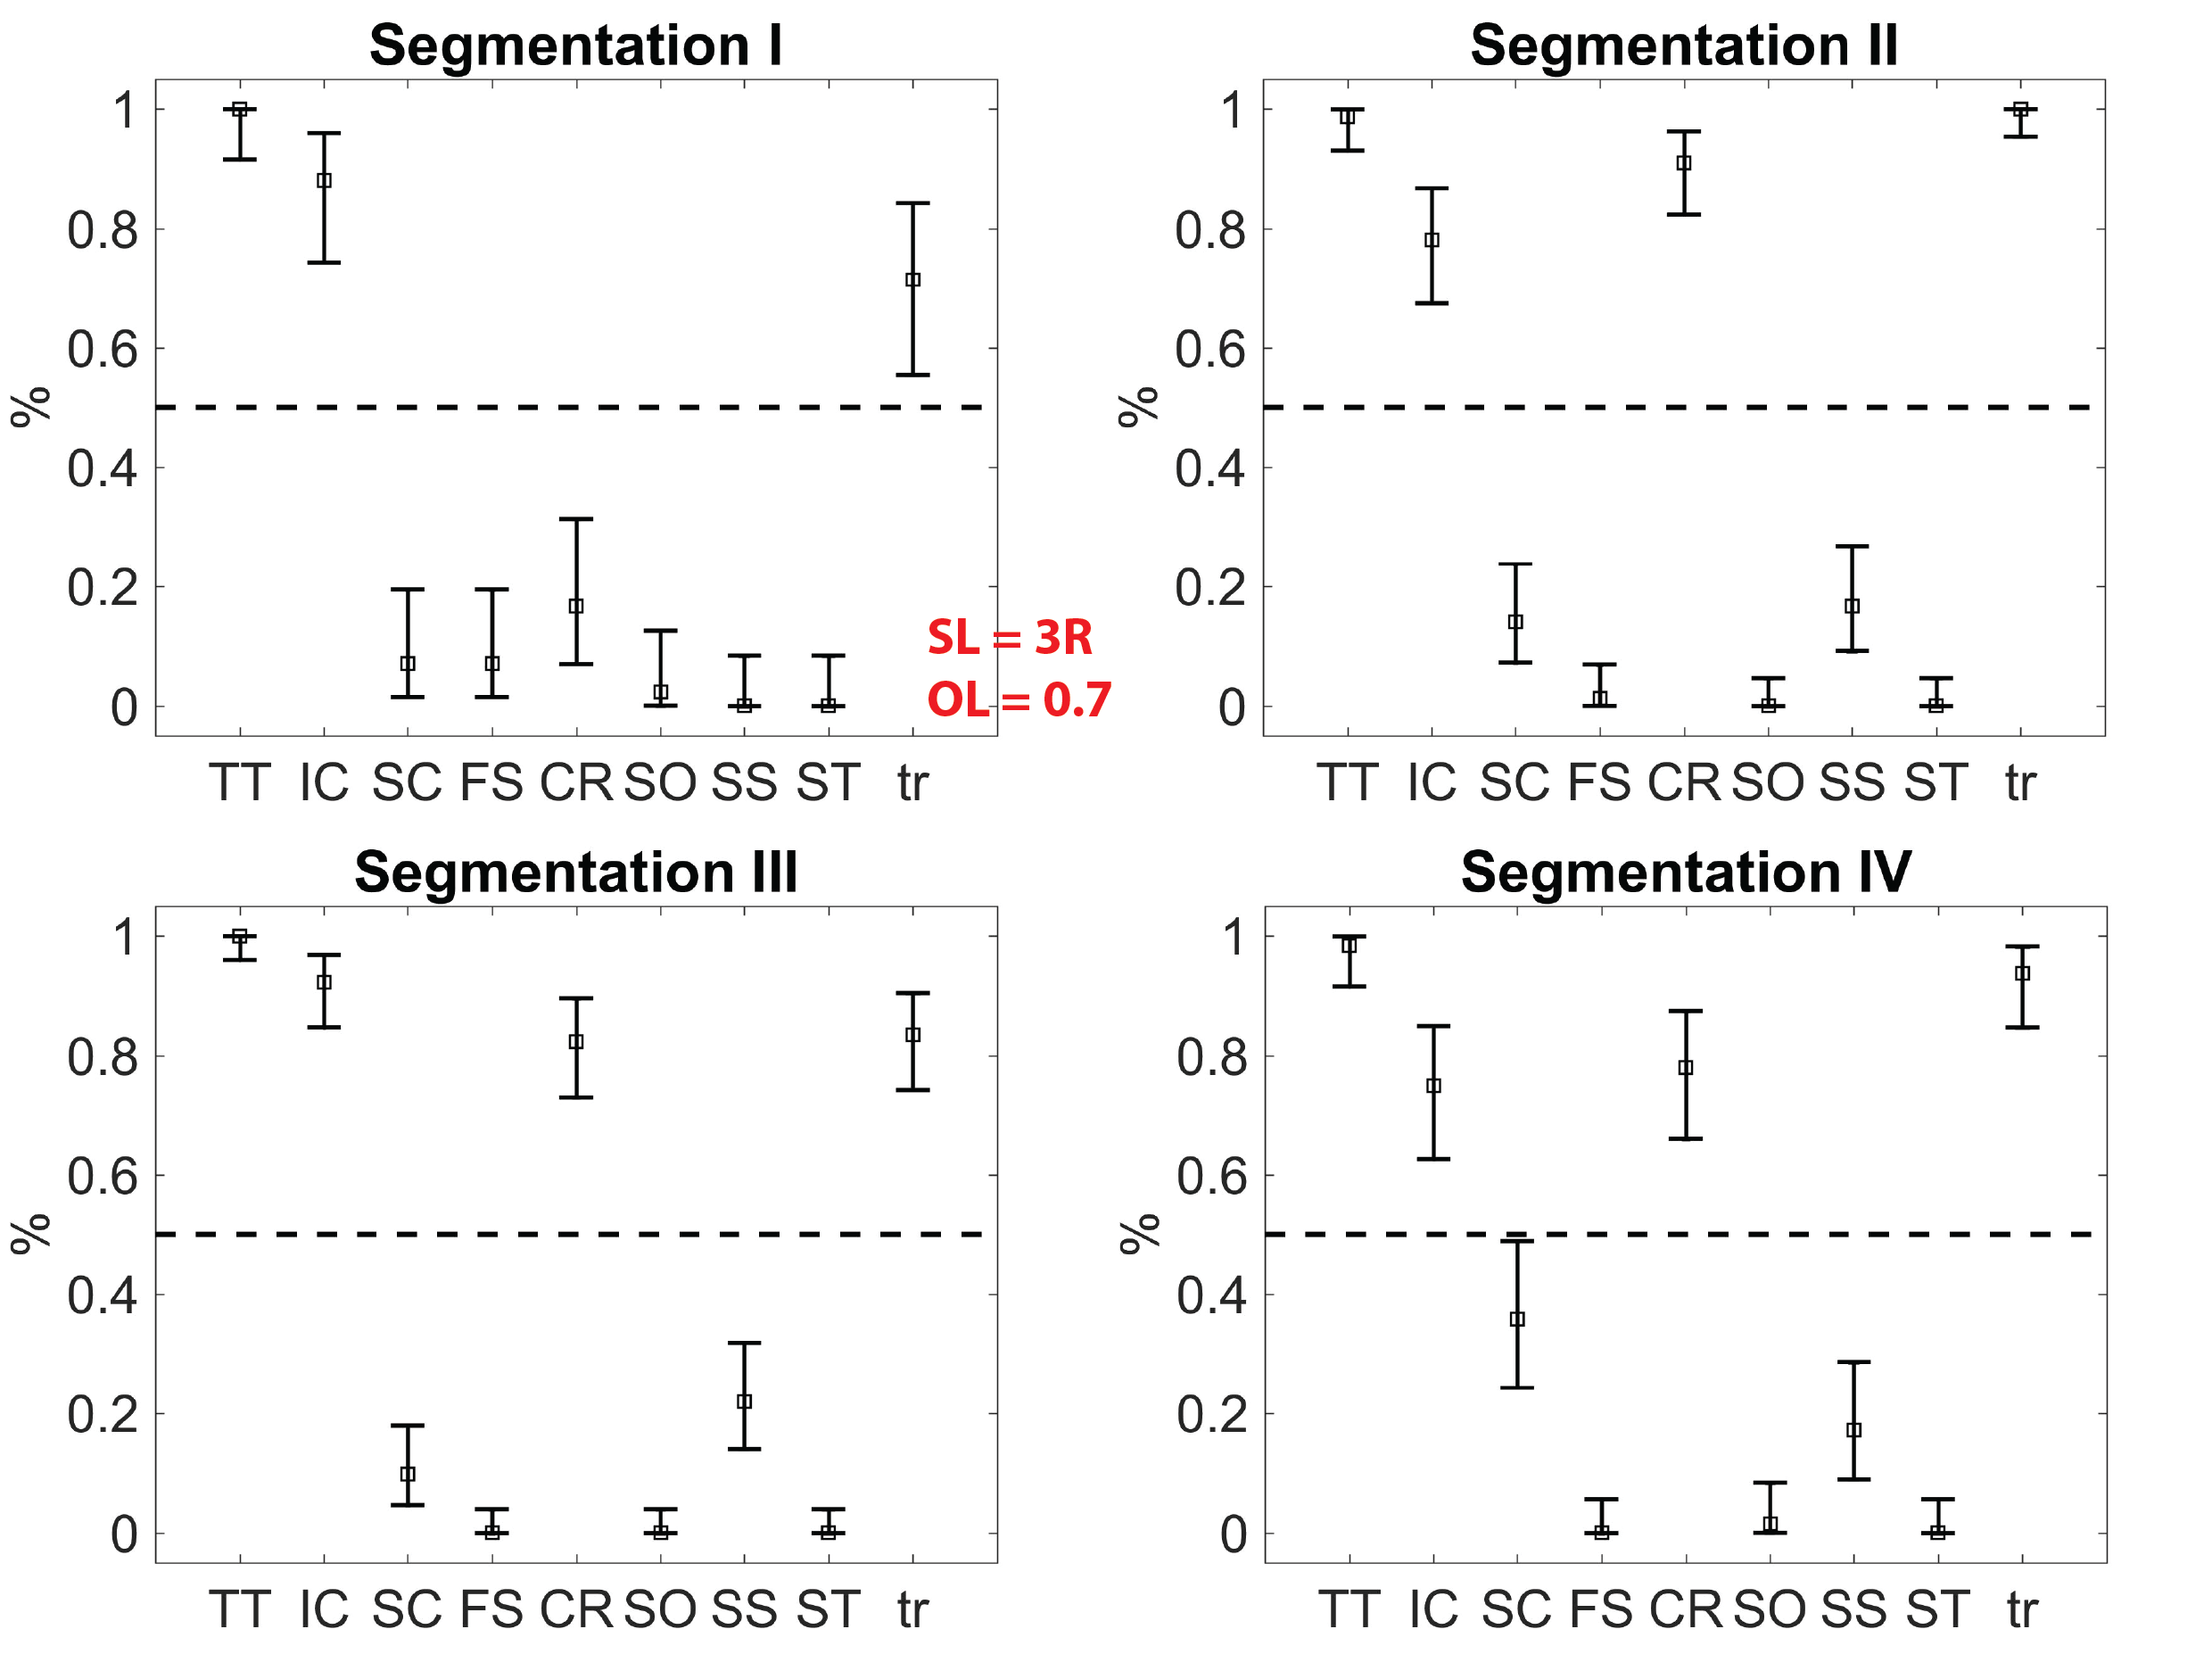
\includegraphics[width=0.85\textwidth]{figures/res4}
	\end{figure}
	\vspace{15mm}
\end{frame}

\begin{frame}{Further validation: EPFL - Stress vs Control Groups}
	\textbf{What about interval length and $\sigma$?}\\ 
	\begin{large}	
		\begin{equation*}
		C_{T_i} \equiv arg_{c_k}max\sum_{\binom{S_j \in c_k}{T_i\cap S_j\neq\varnothing}} w_k \cdot e^{-\frac{d_{ij}^2}{2 \cdot \sigma^2}},
		\textit{\invisible{xxxxx}}w_k = \frac{1}{P(c_k)}
		\end{equation*}	
	\end{large}
	\vspace{3mm}	
	\begin{figure}[H]
		\centering
		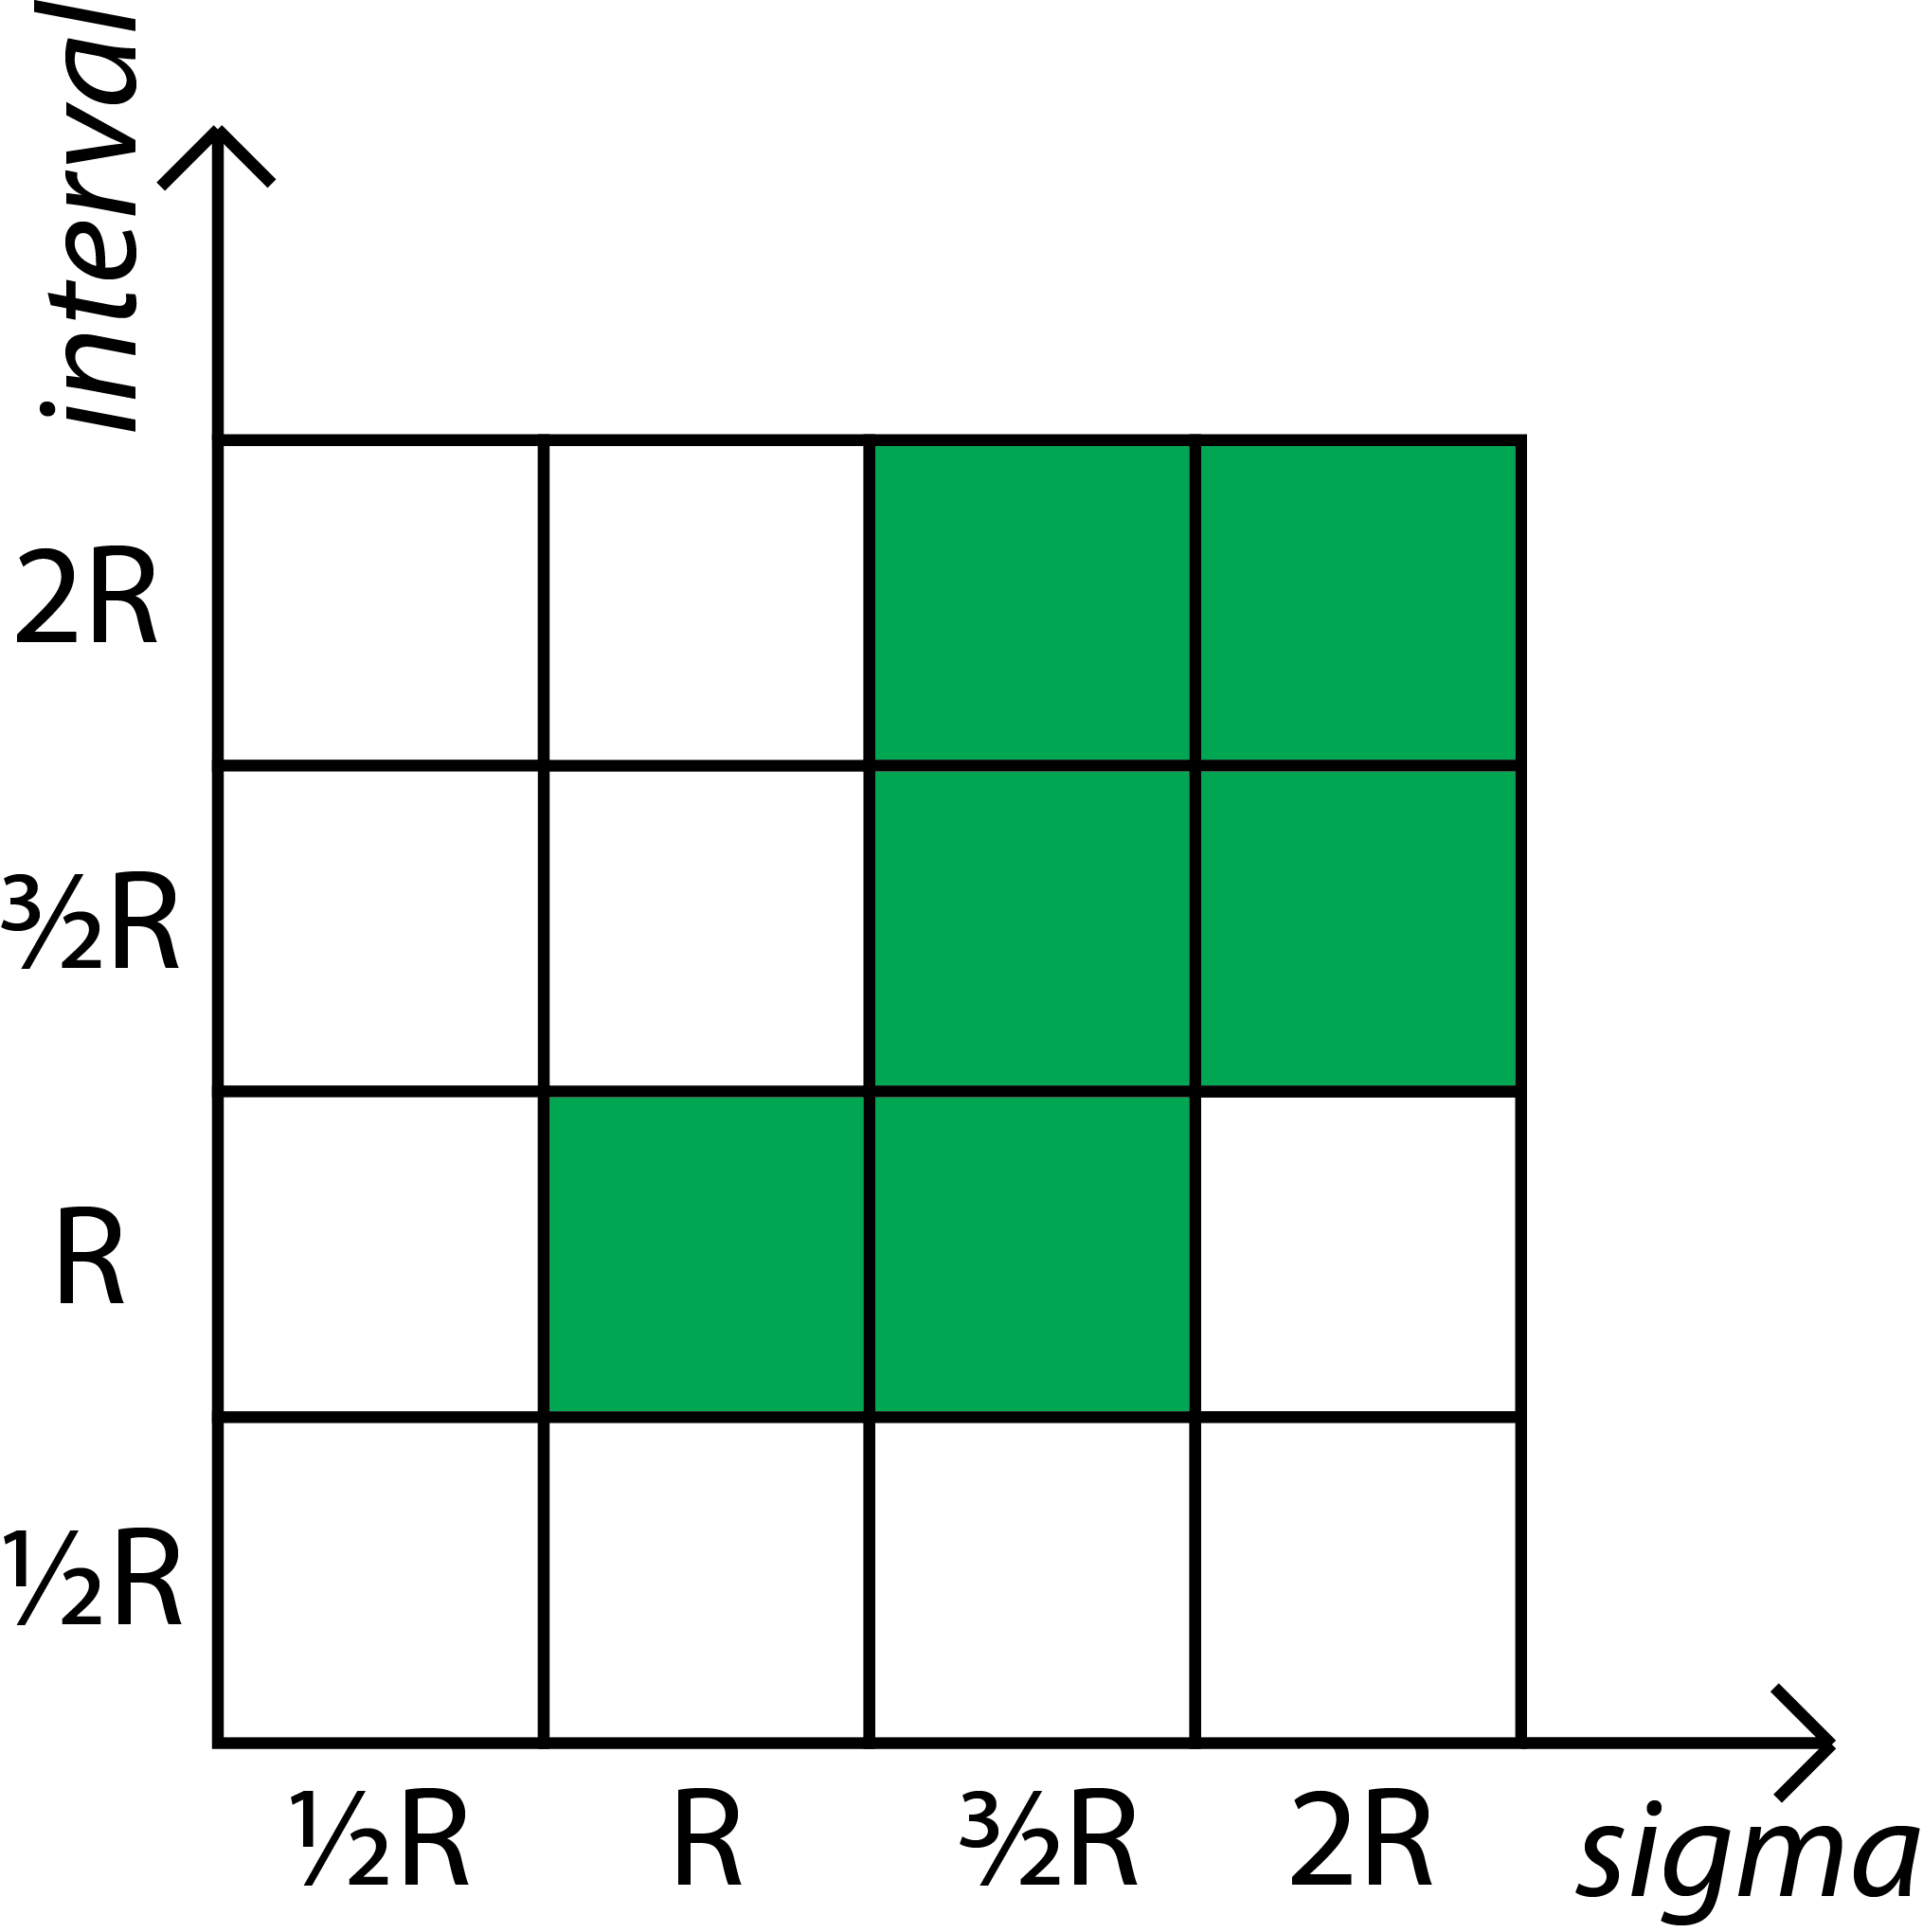
\includegraphics[width=0.4\textwidth]{figures/smoothing}
	\end{figure}
	\vspace{15mm}
\end{frame}

\begin{frame}{Further validation: EPFL - Stress vs Control Groups}
	\textbf{Diversity [1-2], and strength [3-4] of the classifiers?}\\ 
	\vspace{2mm}	
	\begin{figure}[H]
		\centering
		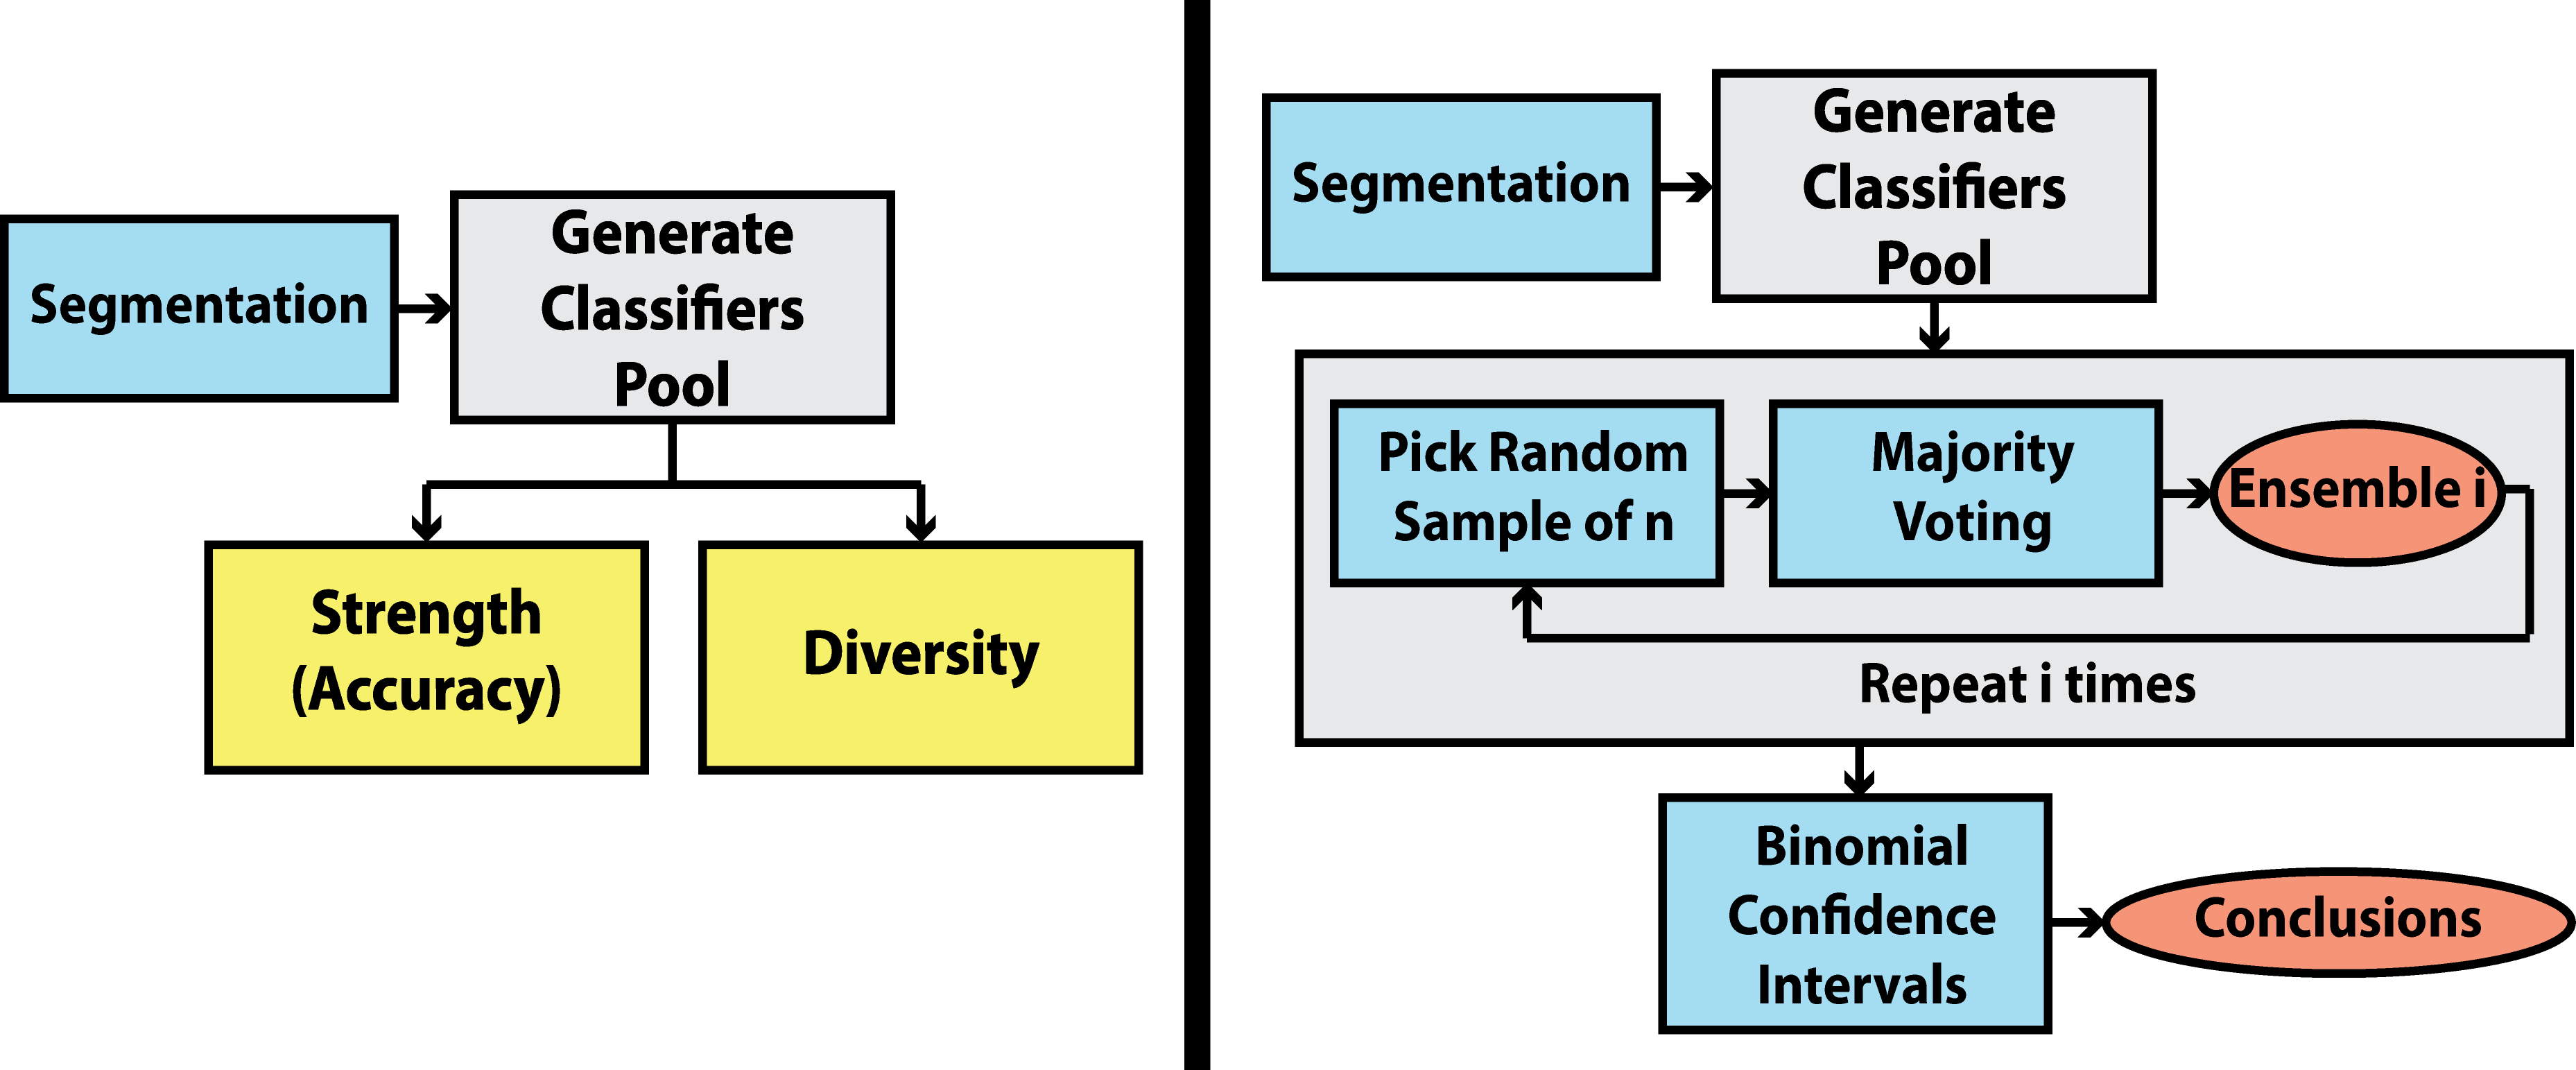
\includegraphics[width=\textwidth]{figures/testing1}
	\end{figure}
	\vspace{1mm}
	\begin{tiny}
		\begin{noindlist}
			\item $[1]$ Gerecke, Uwe, Noel E. Sharkey, and Amanda JC Sharkey. "Common evidence vectors for self-organized ensemble localization." Neurocomputing 55.3-4 (2003): 499-519.
			\item $[2]$ Schapire, Robert E. "The strength of weak learnability." Machine learning 5.2 (1990): 197-227.
			\item $[3]$ Zhu, Mu. "Use of majority votes in statistical learning." Wiley Interdisciplinary Reviews: Computational Statistics 7.6 (2015): 357-371.
			\item $[4]$ Ruta, Dymitr, and Bogdan Gabrys. "A theoretical analysis of the limits of majority voting errors for multiple classifier systems." Pattern Analysis and Applications 5.4 (2002): 333-350.
		\end{noindlist}
	\end{tiny}
\end{frame}
\begin{frame}{Further validation: EPFL - Stress vs Control Groups}
	\textbf{Diversity, and strength of the classifiers?}\\ 
	\vspace{3mm}	
	\begin{figure}[H]
		\centering
		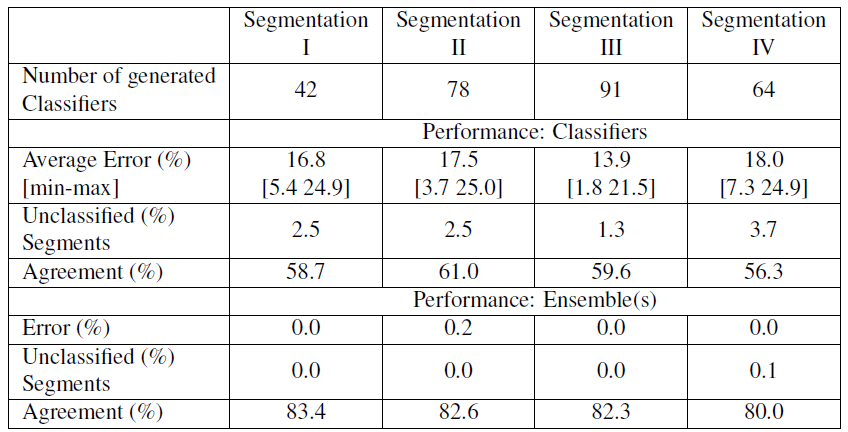
\includegraphics[width=\textwidth]{figures/testing2}
	\end{figure}
	\vspace{15mm}
\end{frame}

\begin{frame}{The RODA Software}	
	\begin{figure}[H]
		\centering
		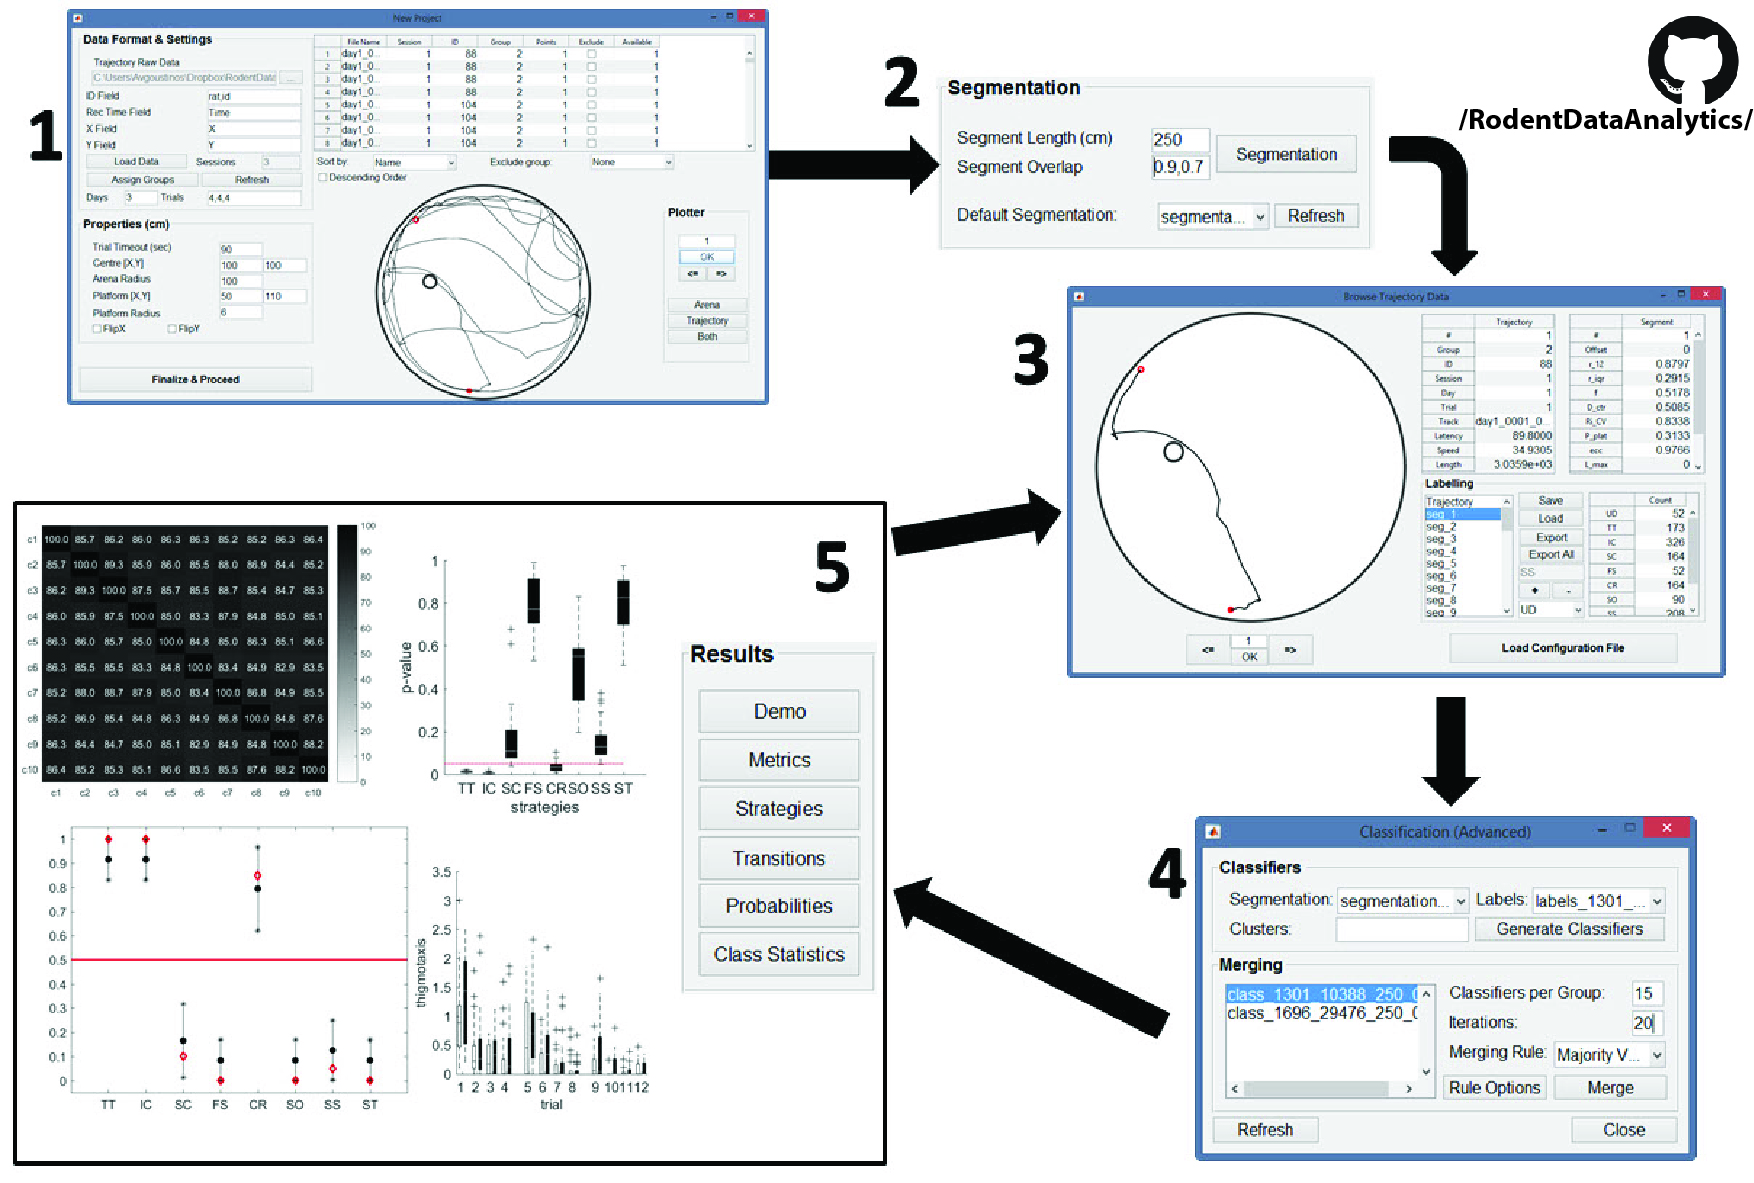
\includegraphics[width=0.95\textwidth]{figures/roda}
	\end{figure}
	\vspace{15mm}
\end{frame}

\begin{frame}{Further applications, requests and Q\&A}	
	\begin{figure}[H]
		\centering
		
\includegraphics[width=0.7\textwidth]{figures/cols}
	\end{figure}
	\begin{itemize}[label={\MyShadow{$\bullet$}{blue!80}}]
		\item Niina Lapinlampi, University of Eastern Finland, A.I. Virtanen Institute for Molecular Sciences, Finland.
		\item Gido Gravesteijn, CADASIL research group, Leiden University Medical Center, Department of Clinical Genetics and Department of Human Genetics, Leiden, The Netherlands.
		\item Richard Pinnell and Ulrich Hofmann Neuroelectronic Systems, Dept. of Neurosurgery, University Medical Centre Freiburg, Freiburg, Germany.
		\item Qazi Rahman, King's College London, Psychology Department, Health Psychology Research Group, UK.
		\item Noam Joseph, Mote Marine Laboratory \& Aquarium, Florida, USA (now in Israel).
	\end{itemize}
\end{frame}

\begin{frame}{Manuscript under peer-review by Scientific Reports}	
	\begin{figure}[H]
		\centering
		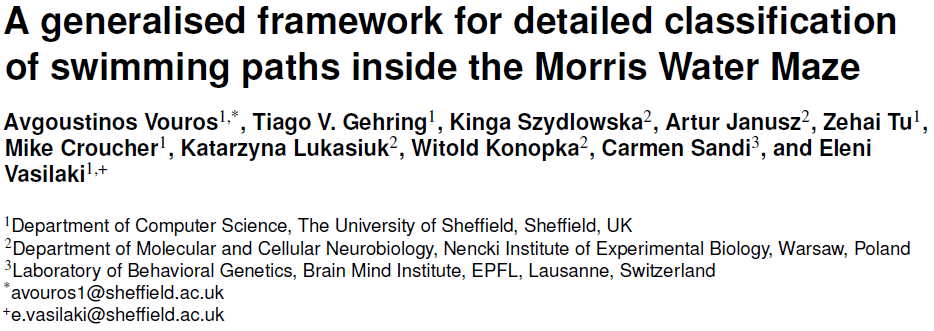
\includegraphics[width=\textwidth]{figures/paper}
	\end{figure}
\end{frame}

%%%%%%%%%%%%%%%%%%%%%%%%%%%%%%%%%%%%%%%%%%%%%%%%%

\begin{frame}[plain,c]
%\frametitle{A first slide}
\begin{center}
	\Huge RODA adaptation to other experimental procedures
\end{center}
\end{frame}

\begin{frame}{RODA adaptation to other experimental procedures}
	\begin{figure}[H]
		\centering
		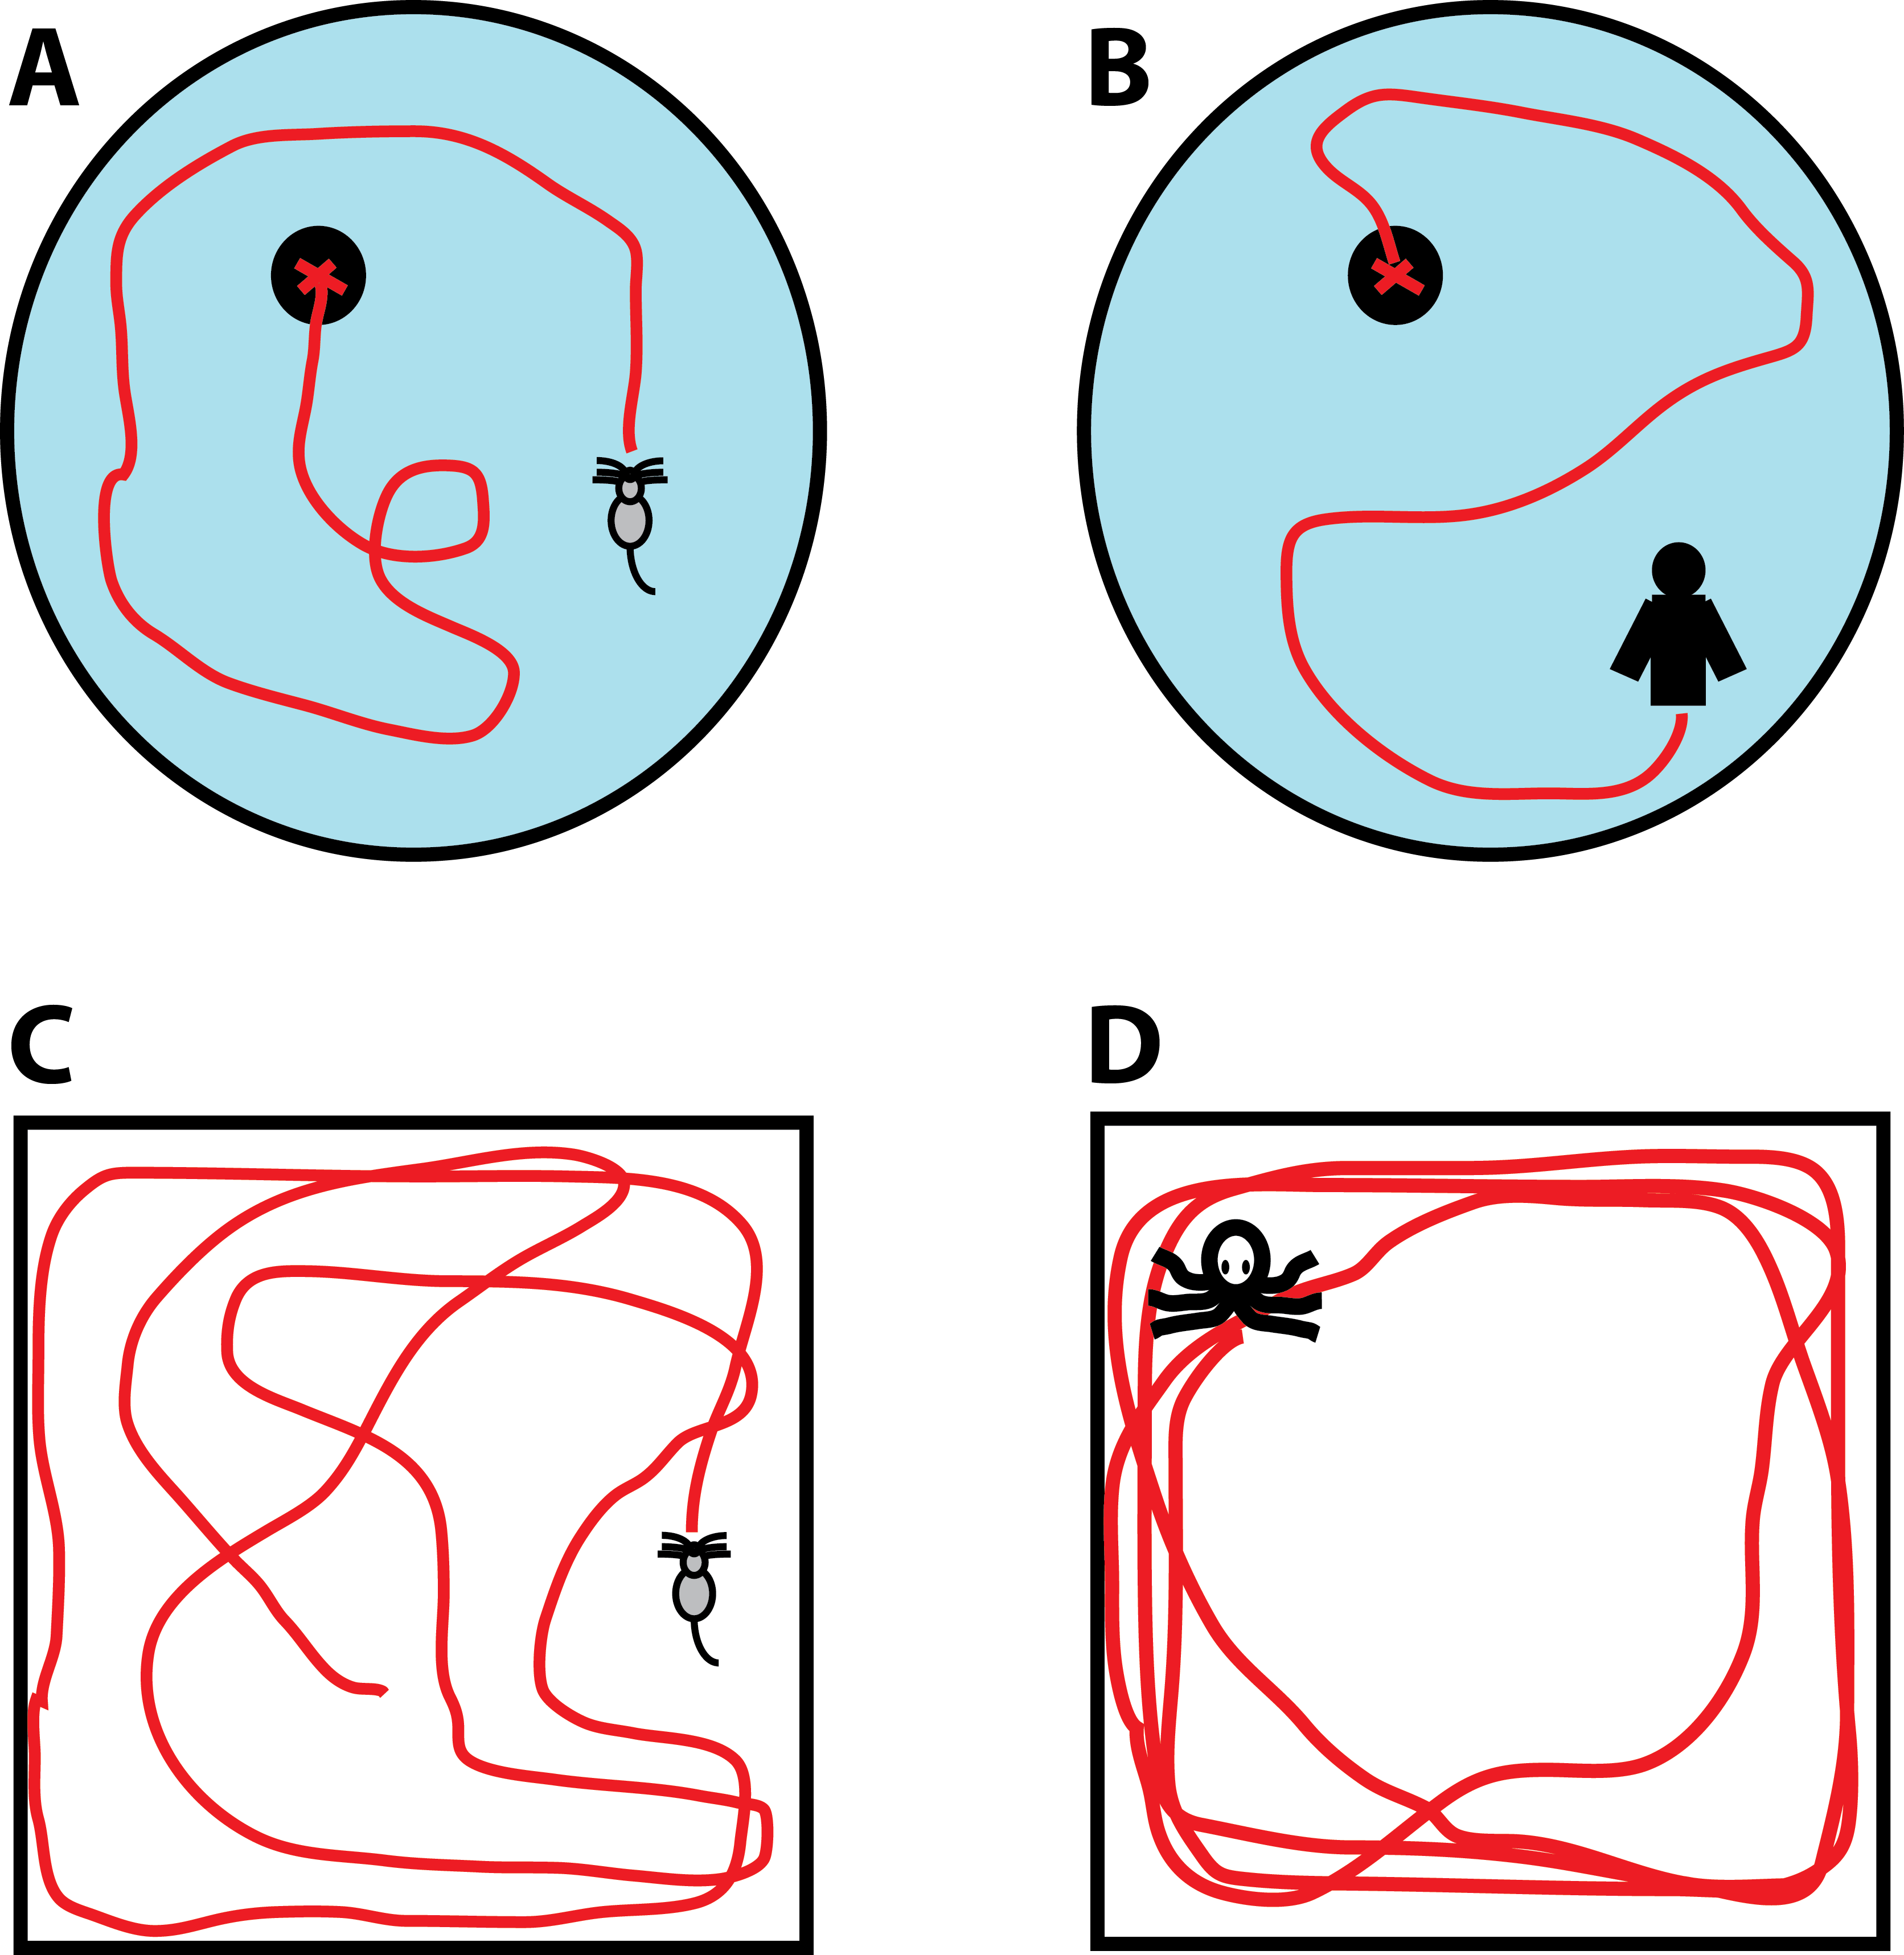
\includegraphics[width=0.6\textwidth]{figures/MWM+OF1}
	\end{figure}
\end{frame}
\begin{frame}{RODA adaptation to other experimental procedures}
	\begin{figure}[H]
		\centering
		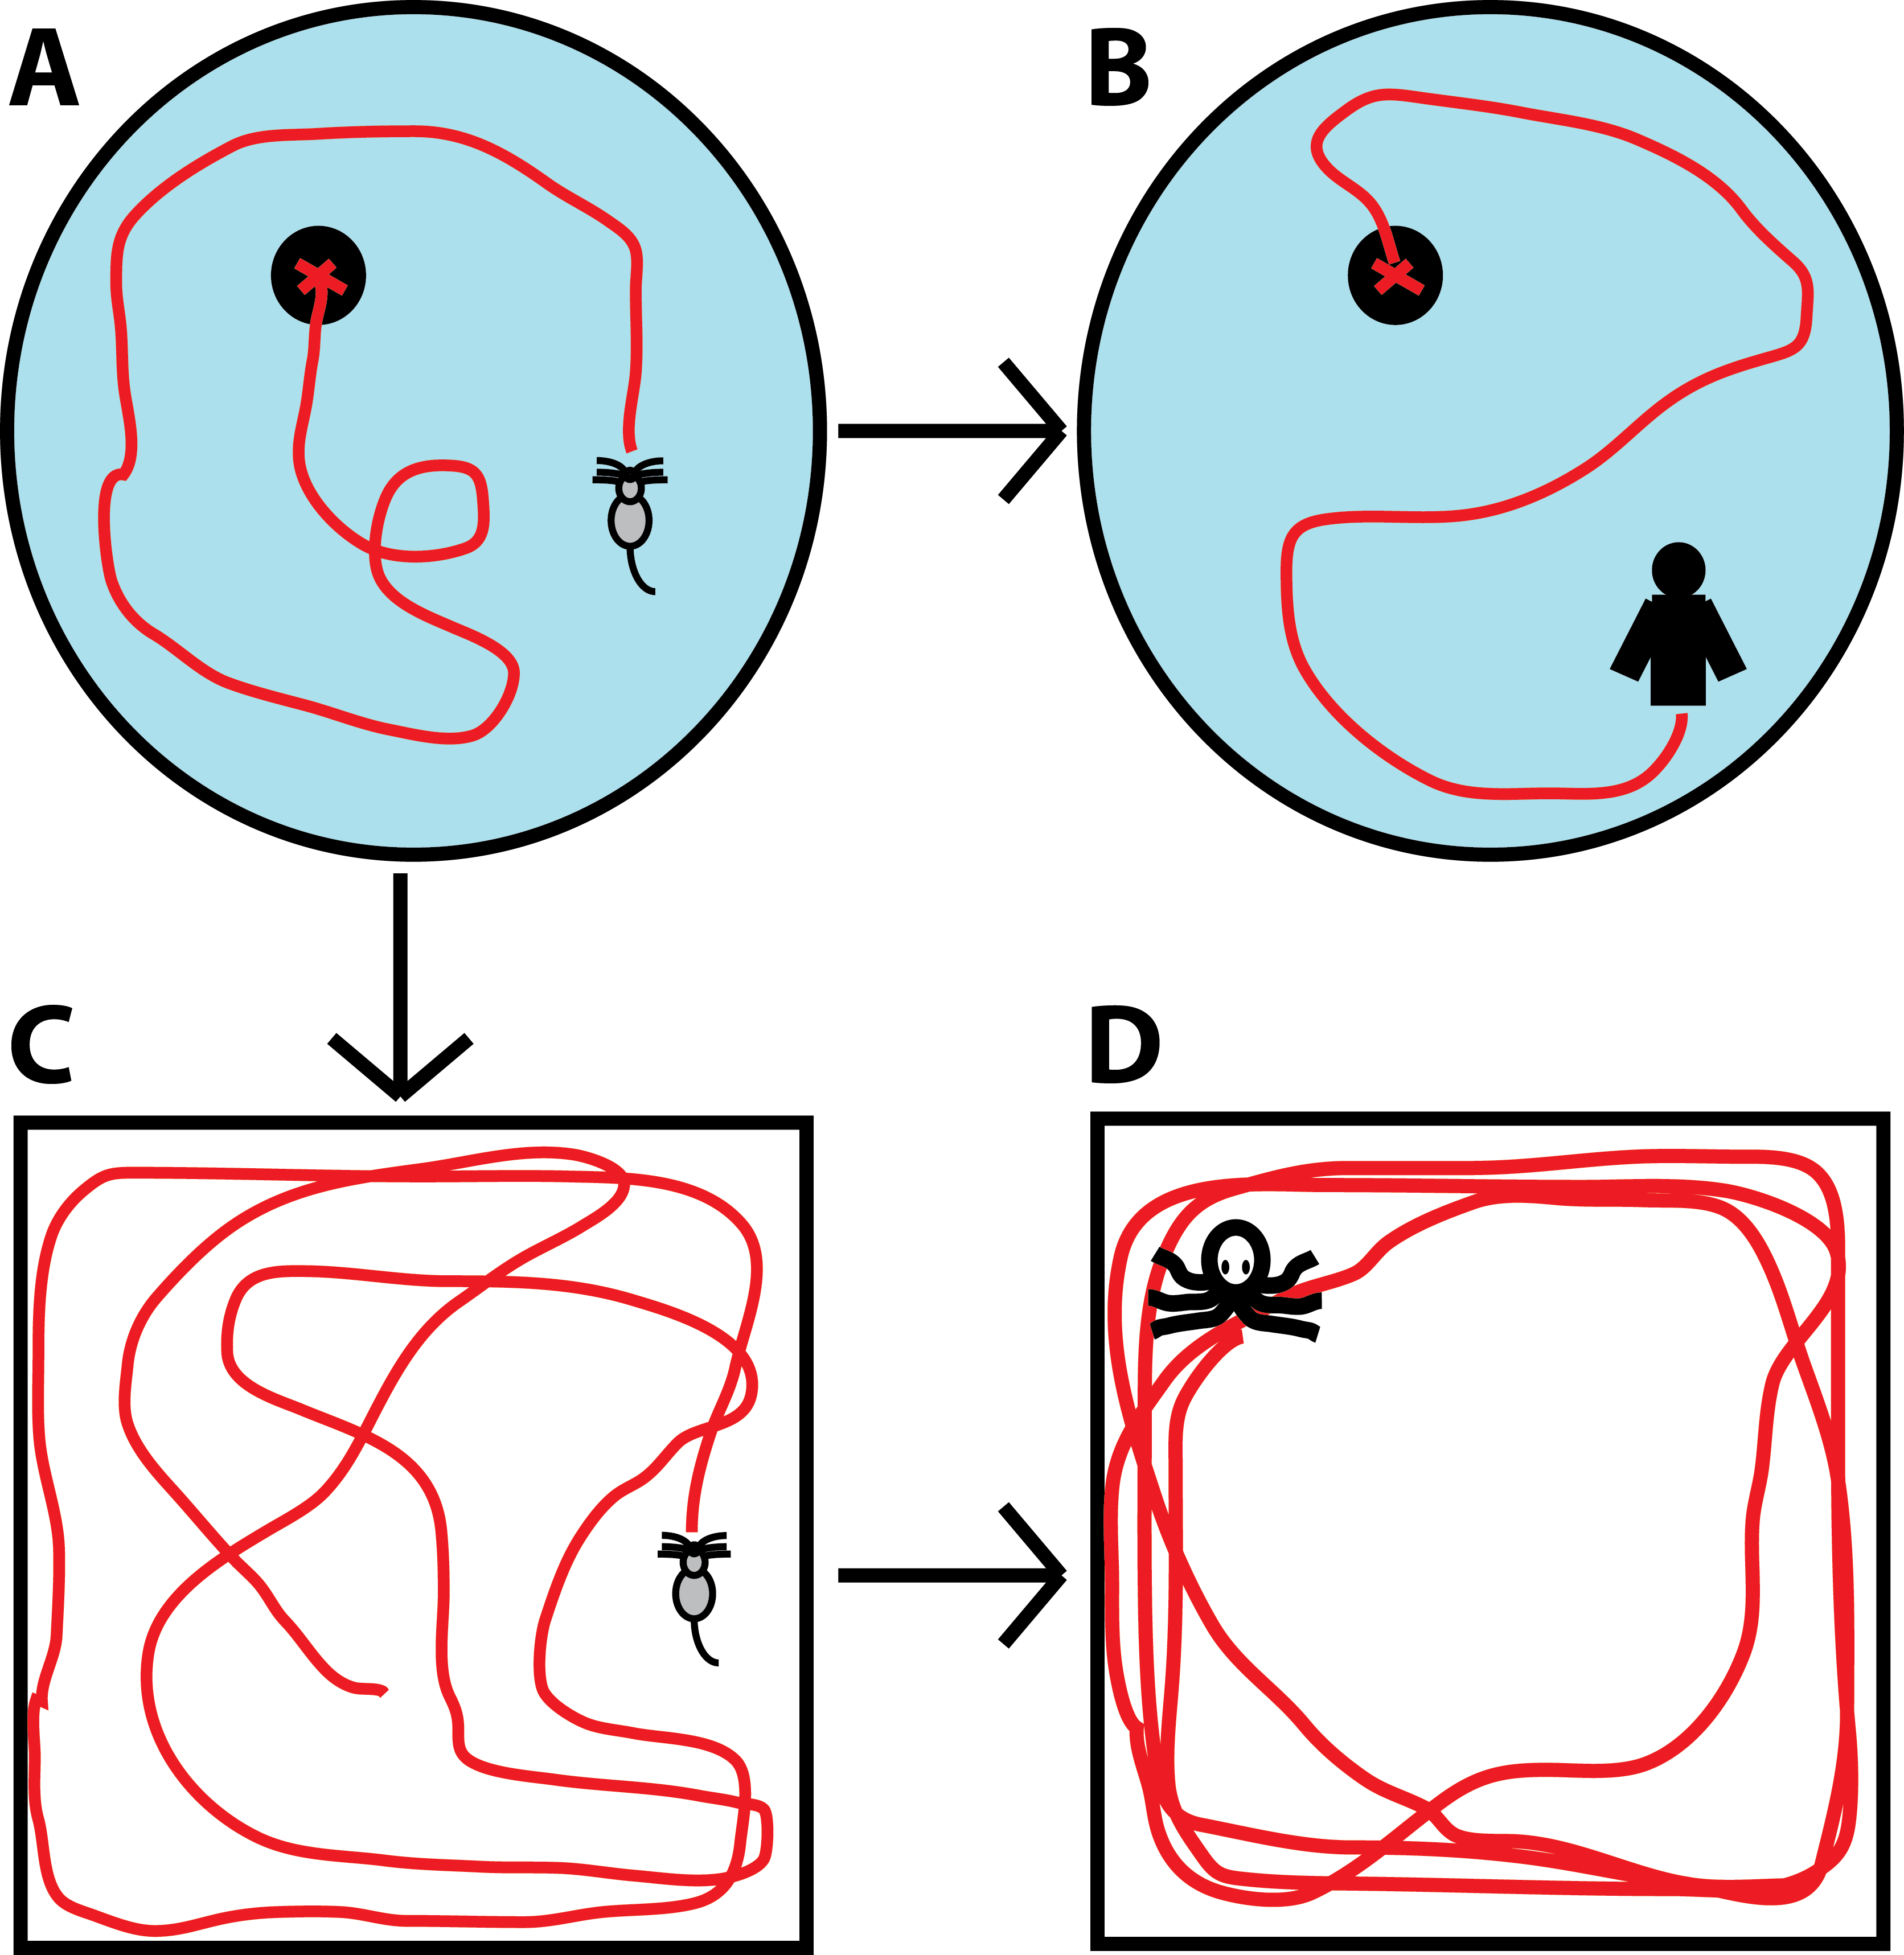
\includegraphics[width=0.6\textwidth]{figures/MWM+OF2}
	\end{figure}
\end{frame}

\begin{frame}{RODA adaptation to other experimental procedures}
	\begin{figure}[H]
		\centering
		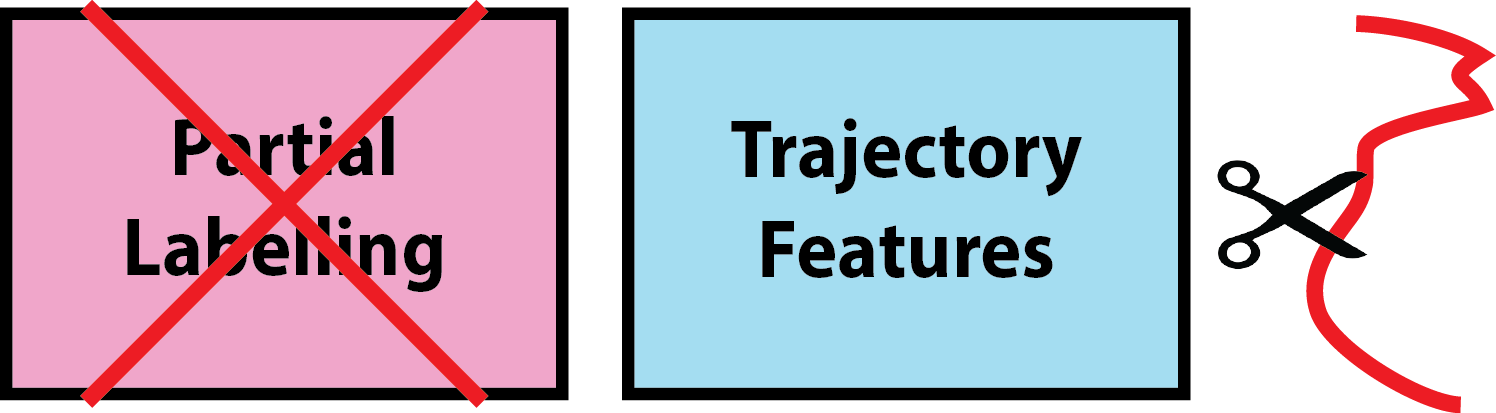
\includegraphics[width=0.6\textwidth]{figures/future}
	\end{figure}
\end{frame}

\begin{frame}{RODA adaptation to other experimental procedures}
	\textbf{Clustering}
	\begin{figure}[H]
		\centering
		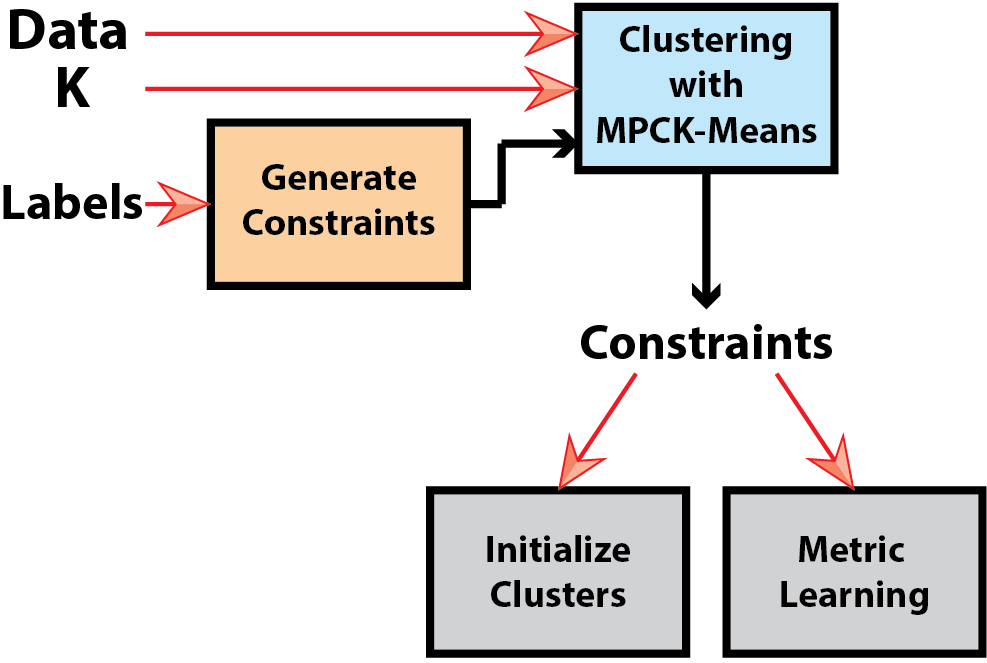
\includegraphics[width=0.8\textwidth]{figures/procMPCKmeans2}
	\end{figure}
\end{frame}
\begin{frame}{RODA adaptation to other experimental procedures}
	\textbf{Clustering}
	\begin{figure}[H]
		\centering
		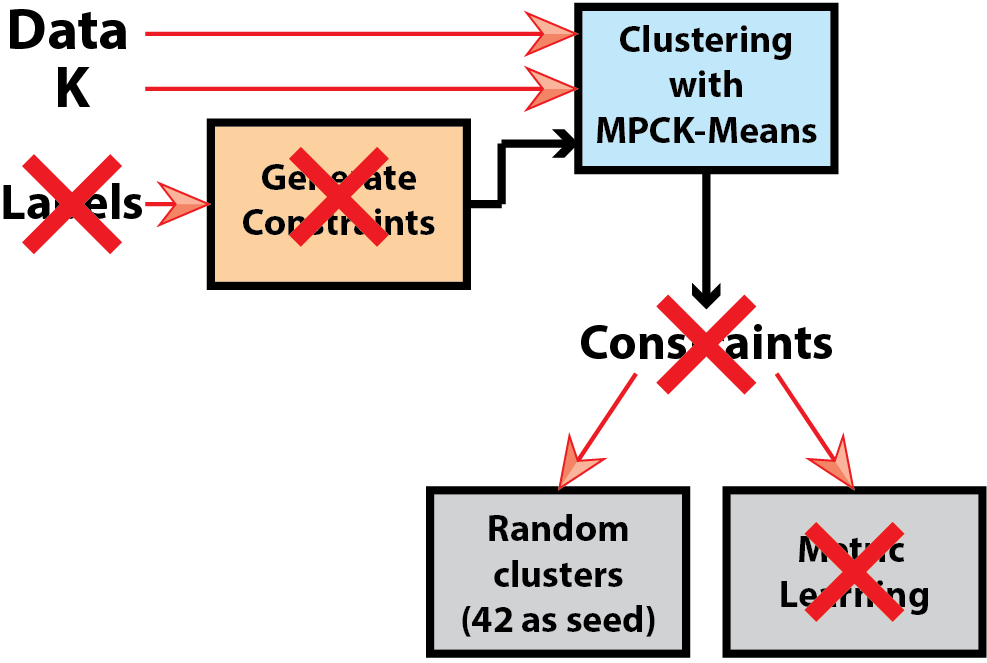
\includegraphics[width=0.8\textwidth]{figures/procMPCKmeans3}
	\end{figure}
\end{frame}

\begin{frame}{RODA adaptation to other experimental procedures}
	\textbf{Path features}
	\begin{figure}[H]
		\centering
		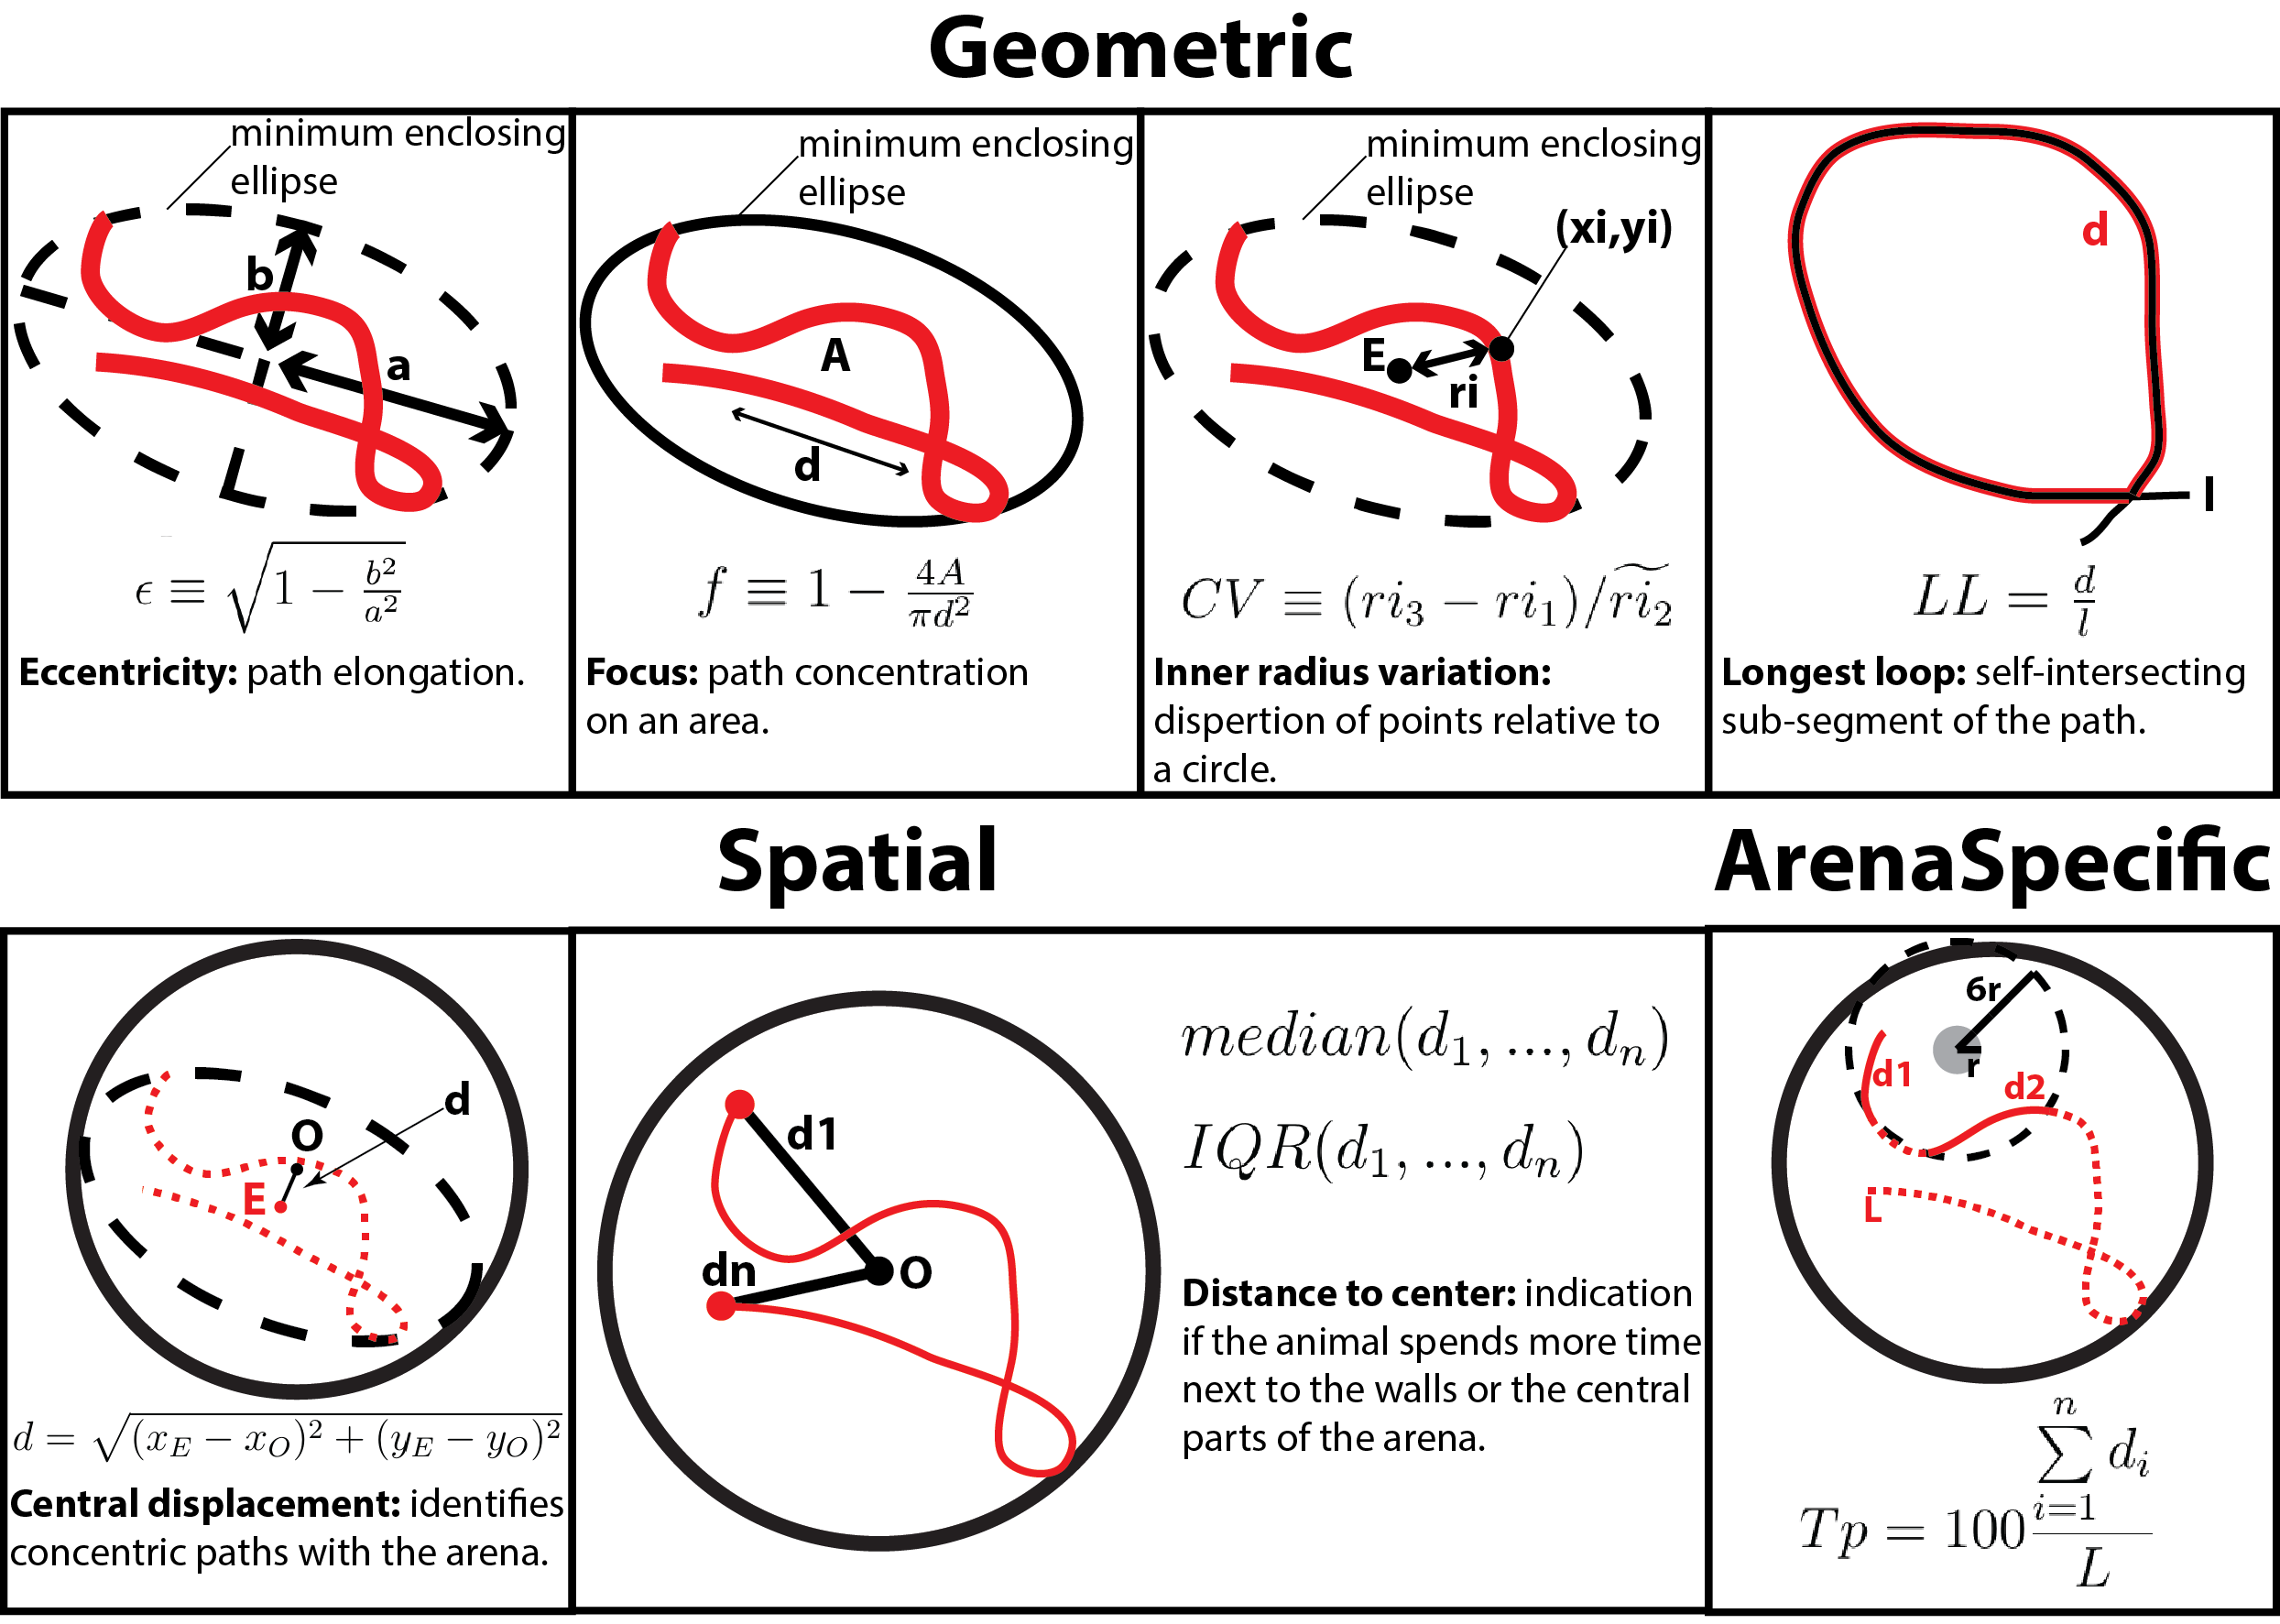
\includegraphics[width=0.87\textwidth]{figures/features2}
	\end{figure}
\end{frame}

\begin{frame}{RODA adaptation to other experimental procedures}
	\textbf{Overlapping segmentation}
	\vspace{18mm}	
	\begin{itemize}[label={\MyShadow{$\bullet$}{blue!80}}]
		\item Generates huge amount of data.
		\vspace{3mm}
		\item Creates difficult to separate data.
		\vspace{3mm}
		\item It cannot capture stationary points.
		%In the open field task rodents are staying in the same position for a significant amount of time probably because they are not stressed by the water.
	\end{itemize}	
	\vspace{30mm}
\end{frame}

\begin{frame}{RODA adaptation to other experimental procedures}
	\textbf{Solutions}	
	\begin{itemize}[label={\MyShadow{$\bullet$}{blue!80}}]
		\item<1-> Implementation of more path features.
		\vspace{3mm}
		\item[\textcolor{red}{$\bullet$}]<2-> A generic segmentation criterion which might be combined with the overlapping segmentation (path sinuosity $[1]$). 
		\vspace{3mm}
		\item<3-> Clustering:
		\vspace{3mm}
		\begin{itemize}[label={\MyShadow{$\bullet$}{blue!80}}]
			\item<3-> Initialize clusters deterministically based on data density (DKMeans++ $[2]$ \textbf{\hyperlink{DKMPP}{\beamerbutton{$\rightarrow$}}}).
			\vspace{3mm}
			\item<4-> Hierarchical clustering (Bisecting K-Means $[3]$).
			\vspace{3mm}
			\item[\textcolor{red}{$\bullet$}]<5-> Feature weighting based on outliers detection and exclusion $[4]$.
			\vspace{3mm}
		\end{itemize}
	\end{itemize}	
	\begin{tiny}
		\begin{noindlist}
			\item<2-> $[1]$ Benhamou, Simon. "How to reliably estimate the tortuosity of an animal's path:: straightness, sinuosity, or fractal dimension?." Journal of theoretical biology 229.2 (2004): 209-220.
			\item<3-> $[2]$ Nidheesh, N., KA Abdul Nazeer, and P. M. Ameer. "An enhanced deterministic K-Means clustering algorithm for cancer subtype prediction from gene expression data." Computers in biology and medicine 91 (2017): 213-221.
			\item<4-> $[3]$ Steinbach, Michael, George Karypis, and Vipin Kumar. "A comparison of document clustering techniques." KDD workshop on text mining. Vol. 400. No. 1. 2000.
			\item<5-> $[4]$ Brodinova, Sarka, et al. "Robust and sparse k-means clustering for high-dimensional data." arXiv preprint arXiv:1709.10012 (2017).
		\end{noindlist}
	\end{tiny}
\end{frame}

\begin{frame}{To be continued...}
	\begin{Large}
		\begin{center}
			\textbf{Thank you for your attention!}
		\end{center}
	\end{Large}	
	\begin{figure}[H]
		\centering
		
\includegraphics[width=0.5\textwidth]{figures/final}
	\end{figure}
	\begin{Large}
		\begin{center}
			\textbf{Any questions?}
		\end{center}
	\end{Large}	
\end{frame}

%\begin{frame}{RODA adaptation to other experimental procedures}
%	\textbf{Issues}
%	\vspace{1mm}	
%	\begin{itemize}
%		\item<1-> The semi-supervised clustering procedure uses the MPCK-Means algorithm which is just K-Means without labels.
%		\begin{itemize}
%			\item<2-> Centroids are initialized based on MUST-LINK constraints else at random using the number 42 as seed.
%			\item<3-> Metric learning depends on MUST-LINK and CANNOT-LINK constraints.
%		\end{itemize}
%		\item<4-> Some features are dependent on the existence of a platform.
%		\item<5-> Overlapping segmentation is a generic method but results in:
%		\begin{itemize}
%			\item<6-> The generation of huge amount of data.
%			\item<7-> Difficult to separate data.
%			\item<8-> It cannot capture stationary points.
%			%In the open field task rodents are staying in the same position for a significant amount of time probably because they are not stressed by the water.
%		\end{itemize}	
%	\end{itemize}
%	\vspace{20mm}
%\end{frame}

\begin{frame}[plain,c]
	%\frametitle{A first slide}
	\vspace{25mm}
	\begin{center}
		\Huge Metric Pairwise-Constrained K-Means (MPCK-Means)
	\end{center}
	\vspace{35mm}
	\begin{tiny}
		\begin{noindlist}
			\item Bilenko, Mikhail, Sugato Basu, and Raymond J. Mooney. "Integrating constraints and metric learning in semi-supervised clustering." Proceedings of the twenty-first international conference on Machine learning. ACM, 2004.
		\end{noindlist}
	\end{tiny}	
\end{frame}

\begin{frame}{The Metric Pairwise-Constrained K-Means (MPCK-Means) algorithm}
	\textbf{Pairwise constraints}
	\vspace{1mm}
	\begin{figure}[H]
		\centering
		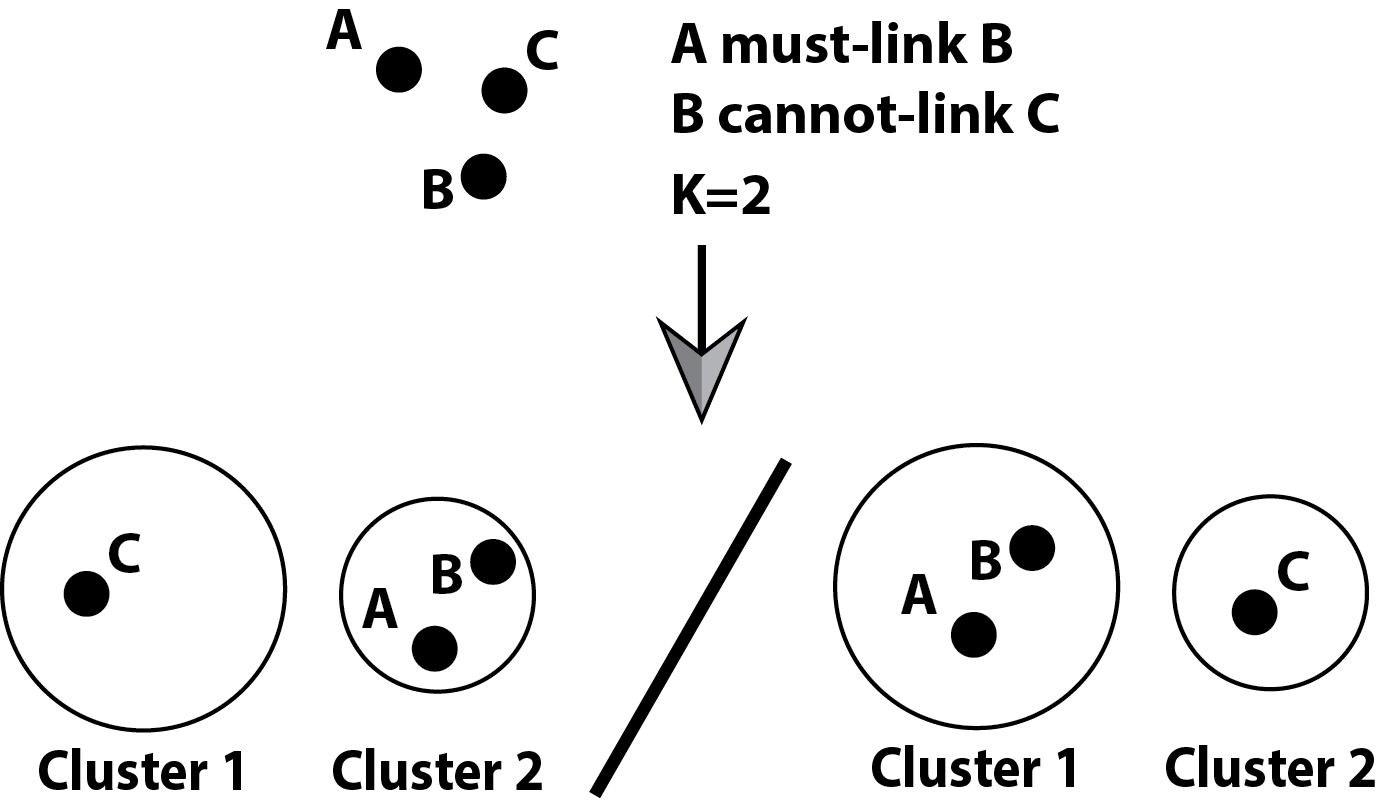
\includegraphics[width=0.6\textwidth]{figures/mpckmeans1}
	\end{figure}
	\vspace{2mm}
	\textbf{Example:} The COP-KMeans; constraints are never broken when updating cluster assignments $[1]$.\\
	\vspace{7mm}
	\begin{tiny}
		\begin{noindlist}
			\item $[1]$ Wagstaff, Kiri, et al. "Constrained k-means clustering with background knowledge." ICML. Vol. 1. 2001.
		\end{noindlist}
	\end{tiny}	
\end{frame}

\begin{frame}{The Metric Pairwise-Constrained K-Means (MPCK-Means) algorithm}
	\textbf{Metric learning}
	\vspace{3mm}	
	\begin{equation}\label{eq1}
		d_A(x_1,x_2) = \lVert x_1 - x_2 \rVert_A = \sqrt{(x_1-x_2)^T A(x_1-x_2)}
	\end{equation}	
	\vspace{3mm}
	\begin{itemize}[label={\MyShadow{$\bullet$}{blue!80}}]
		\item if $A = I$ then (\ref{eq1}) corresponds to the Euclidean distance.
		\vspace{3mm}
		\item if $A$ is diagonal matrix and not $I$ then each axis or dimension is given a weight (feature weighting).
		\vspace{3mm}
		\item if $A$ is full matrix then new features are generated that are linear combination of the original features [2].
	\end{itemize}
	\vspace{5mm}
	\begin{tiny}
		\begin{noindlist}
			\item $[1]$ Xing, Eric P., et al. "Distance metric learning with application to clustering with side-information." Advances in neural information processing systems. 2003.
			\item $[2]$ Basu, Sugato, Mikhail Bilenko, and Raymond J. Mooney. "Comparing and unifying search-based and similarity-based approaches to semi-supervised clustering." Proceedings of the ICML-2003 workshop on the continuum from labeled to unlabeled data in machine learning and data mining. 2003.
		\end{noindlist}
	\end{tiny}	
\end{frame}

\begin{frame}{The Metric Pairwise-Constrained K-Means (MPCK-Means) algorithm}
	\textbf{Initialize cluster centroids}
	\vspace{4mm}
	\begin{itemize}[label={\MyShadow{$\bullet$}{blue!80}}]
		\item<1-> Create $\lambda$ neighborhoods by using the transitive closure of the MUST-LINK constraints.\tab\tab\tab\tab \textbf{\hyperlink{MPCKM}{\beamerbutton{skip explanation}}} %Given a directed graph, find out if a vertex j is reachable from another vertex i for all vertex pairs (i, j) in the given graph. Here reachable mean that there is a path from vertex i to j. The reach-ability matrix is called transitive closure of a graph.
	\end{itemize}
	\begin{multicols}{3}	
	\begin{itemize}
		\item[]<2-> 	
		\begin{figure}[H]
			\centering
			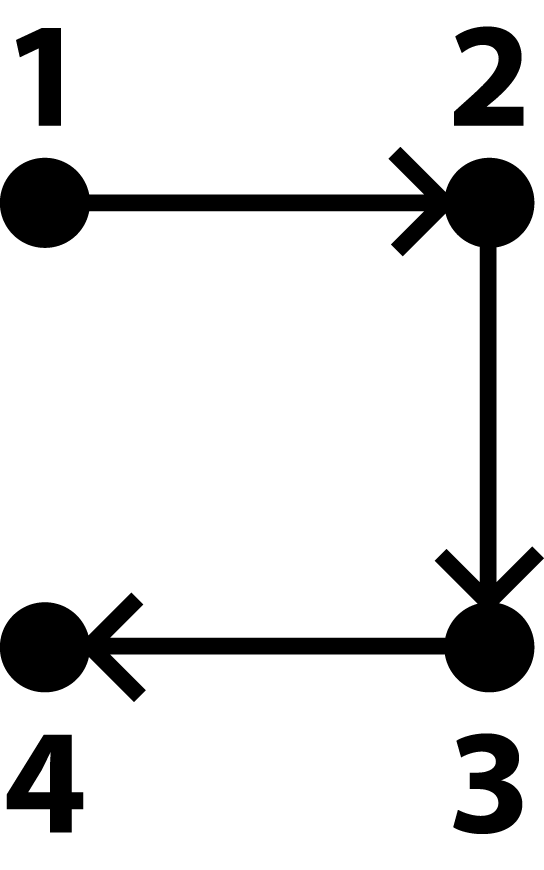
\includegraphics[width=0.1\textwidth]{figures/TransClos1}
		\end{figure}
		\item[]<3-> 	
		\begin{figure}[H]
			\centering
			
\includegraphics[width=0.1\textwidth]{figures/TransClos2}
		\end{figure}
		\item[]<4-> 	
		\begin{figure}[H]
			\centering
			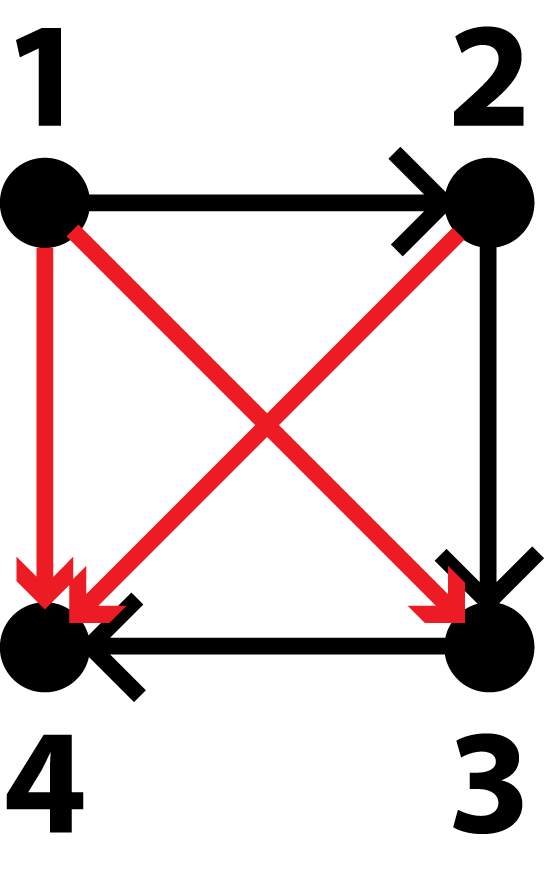
\includegraphics[width=0.1\textwidth]{figures/TransClos3}
		\end{figure}		
	\end{itemize}
	\end{multicols}
	\begin{itemize}[label={\MyShadow{$\rhd$}{blue!80}}]
		\item<5-> $L = \{(1,2),(2,3),(3,4)\}$\\ \tab$\oplus$ $\{(1,3),(2,4)\}$\\ \tab$\oplus$ $\{(1,4)\}$
	\end{itemize}
\end{frame}	

\begin{frame}{The Metric Pairwise-Constrained K-Means (MPCK-Means) algorithm}\label{MPCKM}
	\textbf{Initialize cluster centroids}
	\vspace{4mm}
	\begin{itemize}[label={\MyShadow{$\bullet$}{blue!80}}]
		\item Create $\lambda$ neighborhoods by using the transitive closure of the MUST-LINK constraints. %Given a directed graph, find out if a vertex j is reachable from another vertex i for all vertex pairs (i, j) in the given graph. Here reachable mean that there is a path from vertex i to j. The reach-ability matrix is called transitive closure of a graph.
		\vspace{3mm}
		\item Augment the MUST-LINK and CANNOT-LINK sets of constraints with any additional constraints. %e.g. if two neighborhoods $l_1$ and $l_2$ have at least one CANNOT-LINK constraint between them then create CANNOT-LINK constrains between all the data points of $l_1$ and $l_2$.
		\vspace{3mm}
		\item Use the centers of the neighborhoods as centroids:
		\begin{itemize}[label={\MyShadow{$\circ$}{blue!80}}]
			\item if $k = \lambda$ initialize $\lambda$ centroids.
			\vspace{3mm}
			\item if $k > \lambda$ initialize $\lambda$ centroids and the remaining $k - \lambda$ centroids at random \textit{using \textbf{$42$} as random seed}.	
			\vspace{3mm}	
			\item if $k < \lambda$ initialize $k$ neighborhoods from $\lambda$ based on weighted farthest-first traversal where the weights are the sizes of the neighborhoods. 
			%Weighted farthest-first traversal: Find K points which are maximally separated from each other in terms of a weighted distance.
			%Thus the $k$ neighborhoods which are far apart but also large are selected.
		\end{itemize}		
	\vspace{6mm}			
	\end{itemize}	
	\vspace{6mm}	
\end{frame}	

\begin{frame}{The Metric Pairwise-Constrained K-Means (MPCK-Means) algorithm}
	\textbf{(Weighted) farthest-first traversal}\\
	\vspace{4mm}
	Goal: find K points which are maximally separated from each other (in terms of a weighted distance).
	\vspace{10mm}
	\begin{itemize}[leftmargin=-2mm]
		\setlength\itemsep{2.3em}
		\item[]<1-> 	
		\begin{figure}[H]
			\centering
			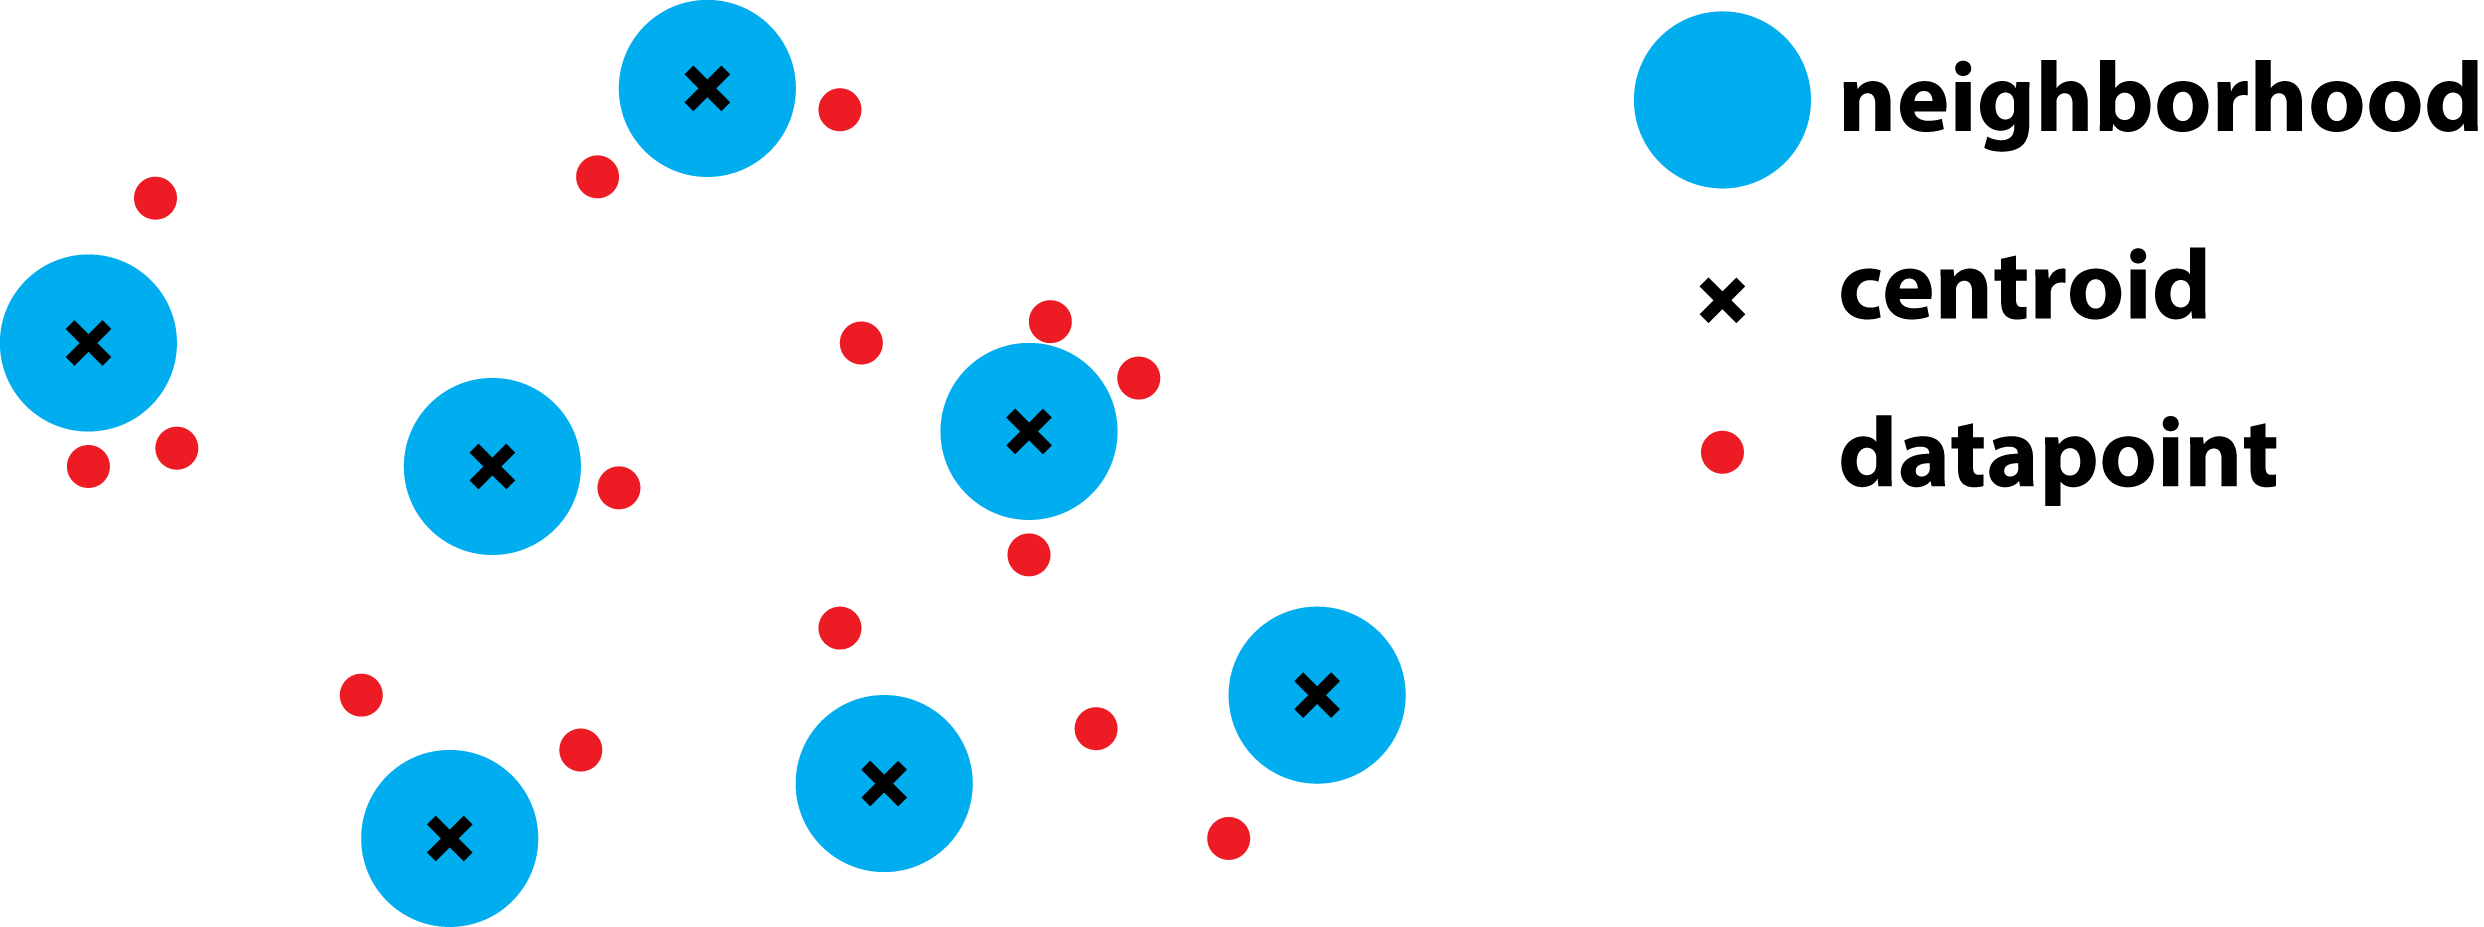
\includegraphics[width=0.7\textwidth]{figures/farthest_setup}
		\end{figure}
	\end{itemize}
	\vspace{14mm}
\end{frame}	
\begin{frame}{The Metric Pairwise-Constrained K-Means (MPCK-Means) algorithm}
	\textbf{(Weighted) farthest-first traversal}\\
	\vspace{4mm}
	\begin{figure}[H]
		\centering
		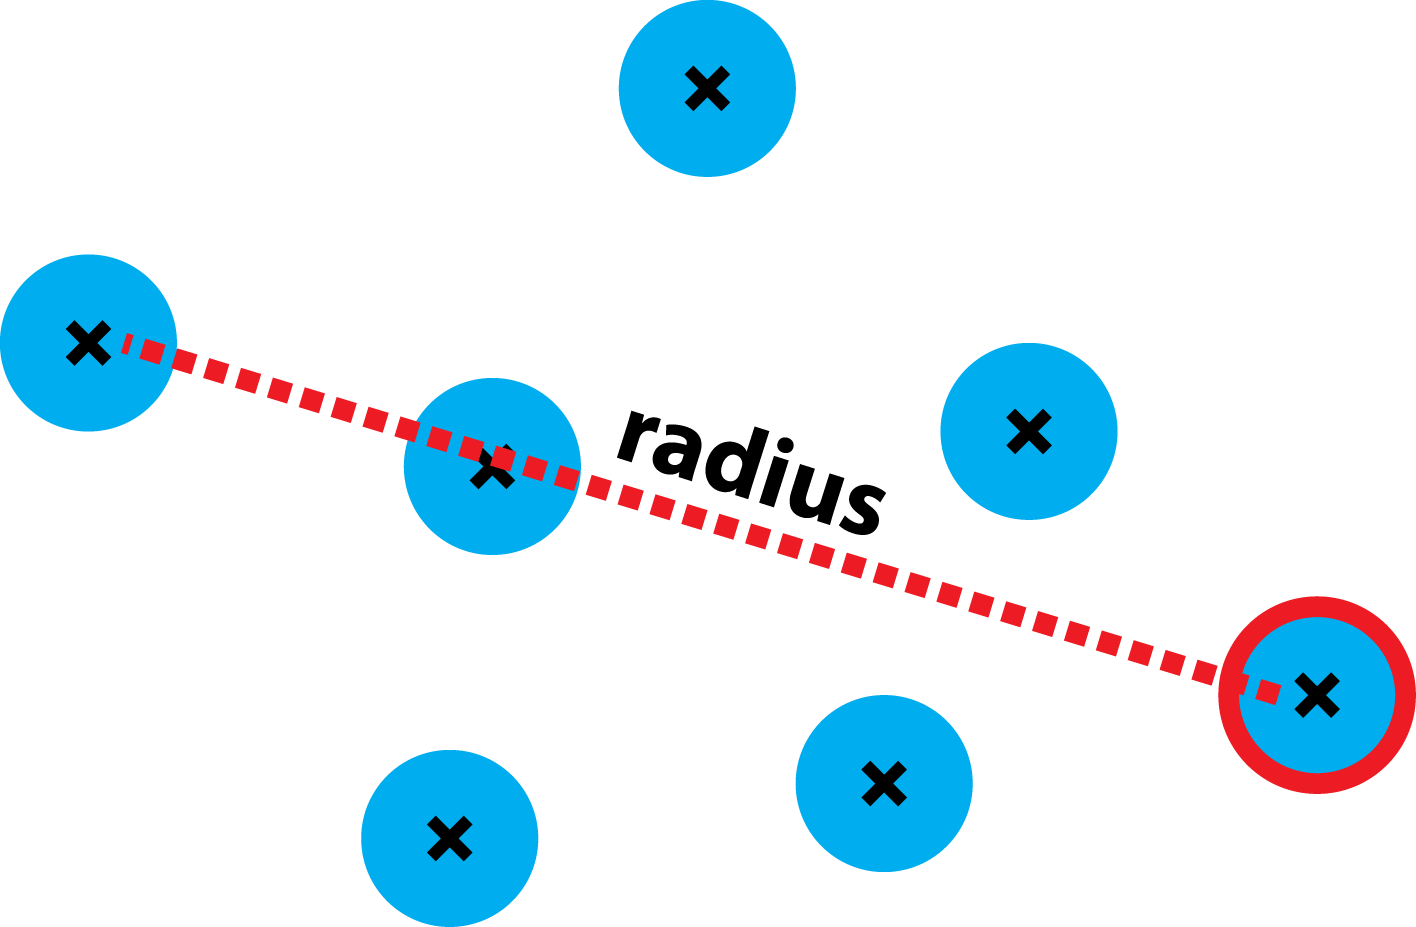
\includegraphics[width=0.4\textwidth]{figures/farthest_1st}
	\end{figure}
	\vspace{2mm}
	\begin{itemize}[label={\MyShadow{$\bullet$}{blue!80}}]
		\item<1-> Pick a neighborhood at random $\lambda_1$
		\vspace{3mm}
		\item<1-> Find the furthest neighborhood of $\lambda_1$.	
	\end{itemize}	
	\vspace{24mm}
\end{frame}	
\begin{frame}{The Metric Pairwise-Constrained K-Means (MPCK-Means) algorithm}
	\textbf{(Weighted) farthest-first traversal}\\
	\vspace{4mm}
	\begin{figure}[H]
		\centering
		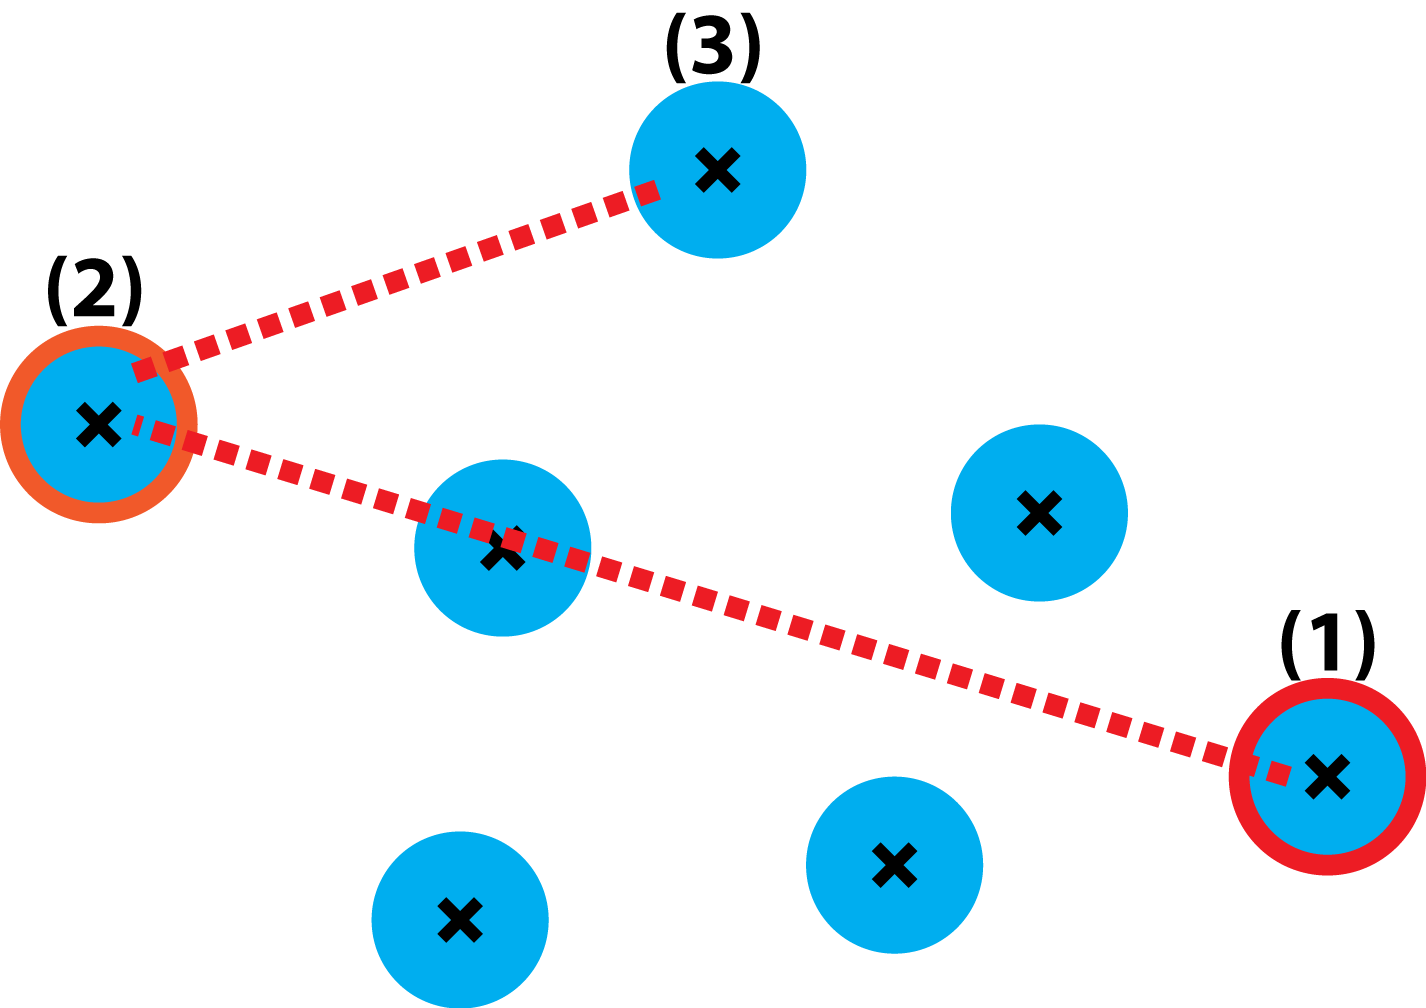
\includegraphics[width=0.4\textwidth]{figures/farthest_2nd}
	\end{figure}
	\vspace{2mm}
	\begin{itemize}[label={\MyShadow{$\bullet$}{blue!80}}]
		\item<1-> Find the furthest neighborhood of $\lambda_2$ that is also the farthest from the neighborhood $\lambda_1$.	
		\vspace{3mm}
		\item<2-> Since $weights \equiv size(\lambda)$, the selected points are far apart and inside large neighborhoods.
	\end{itemize}	
	\vspace{24mm}
\end{frame}	


\begin{frame}{The Metric Pairwise-Constrained K-Means (MPCK-Means) algorithm}
	\textbf{Integrating constraints and metric learning}
	\setcounter{equation}{0}
	\begin{align}\label{eq2}
		J &= \sum_{x_i \in X} (\lVert x_i - \mu_{l_i} \rVert_{A_{l_i}}^2 -log(det(A_{l_i}))  ) \\
		& + \sum_{(x_i,x_j)\in M}w_{ij}f_M(x_i,x_j)\mathbbm{1}[l_i \neq l_j] \\
		& + \sum_{(x_i,x_j)\in C}\overline{w}_{ij}f_C(x_i,x_j)\mathbbm{1}[l_i = l_j] %\textit{\vphantom{xxx}, w_{ij} = {w}_{ij} = 1}		
	\end{align}	
	\begin{itemize}
		\item<2-> (1) results in the learning of the diagonal matrix $A$. 
		\item<2-> (2) is the penalty cost of violating the MUST-LINK constraints.
		\item<2-> (3) is the penalty cost of violating the CANNOT-LINK constraints.
	\end{itemize}	
	\begin{itemize}[label={\MyShadow{$\bullet$}{blue!80}}]
		\item<3-> Severity of M: $f_M = \frac{1}{2}\lVert x_i - x_j \rVert_{A_{l_i}}^2 + \frac{1}{2}\lVert x_i - x_j \rVert_{A_{l_j}}^2$
		\item<3-> Severity of C: $f_M = \lVert x_{l_i}' - x_{l_i}'' \rVert_{A_{l_i}}^2 + \lVert x_i - x_j \rVert_{A_{l_i}}^2$, where $x_{l_i}'$ and $x_{l_i}''$ is the maximally separated pair of points in the dataset.		
	\end{itemize}		
\end{frame}

\begin{frame}[plain,c]\label{DKMPP}
	%\frametitle{A first slide}
	\vspace{25mm}
	\begin{center}
		\Huge Density K-Means++ (DKM++)
	\end{center}
	\vspace{35mm}
	\begin{tiny}
		\begin{noindlist}
			\item Nidheesh, N., KA Abdul Nazeer, and P. M. Ameer. "An enhanced deterministic K-Means clustering algorithm for cancer subtype prediction from gene expression data." Computers in biology and medicine 91 (2017): 213-221.
		\end{noindlist}
	\end{tiny}	
\end{frame}

\begin{frame}{The Density K-Means++ (DKM++) algorithm}
\textbf{Minimum spanning tree}
	\vspace{10mm}
	\begin{figure}[H]
		\centering
		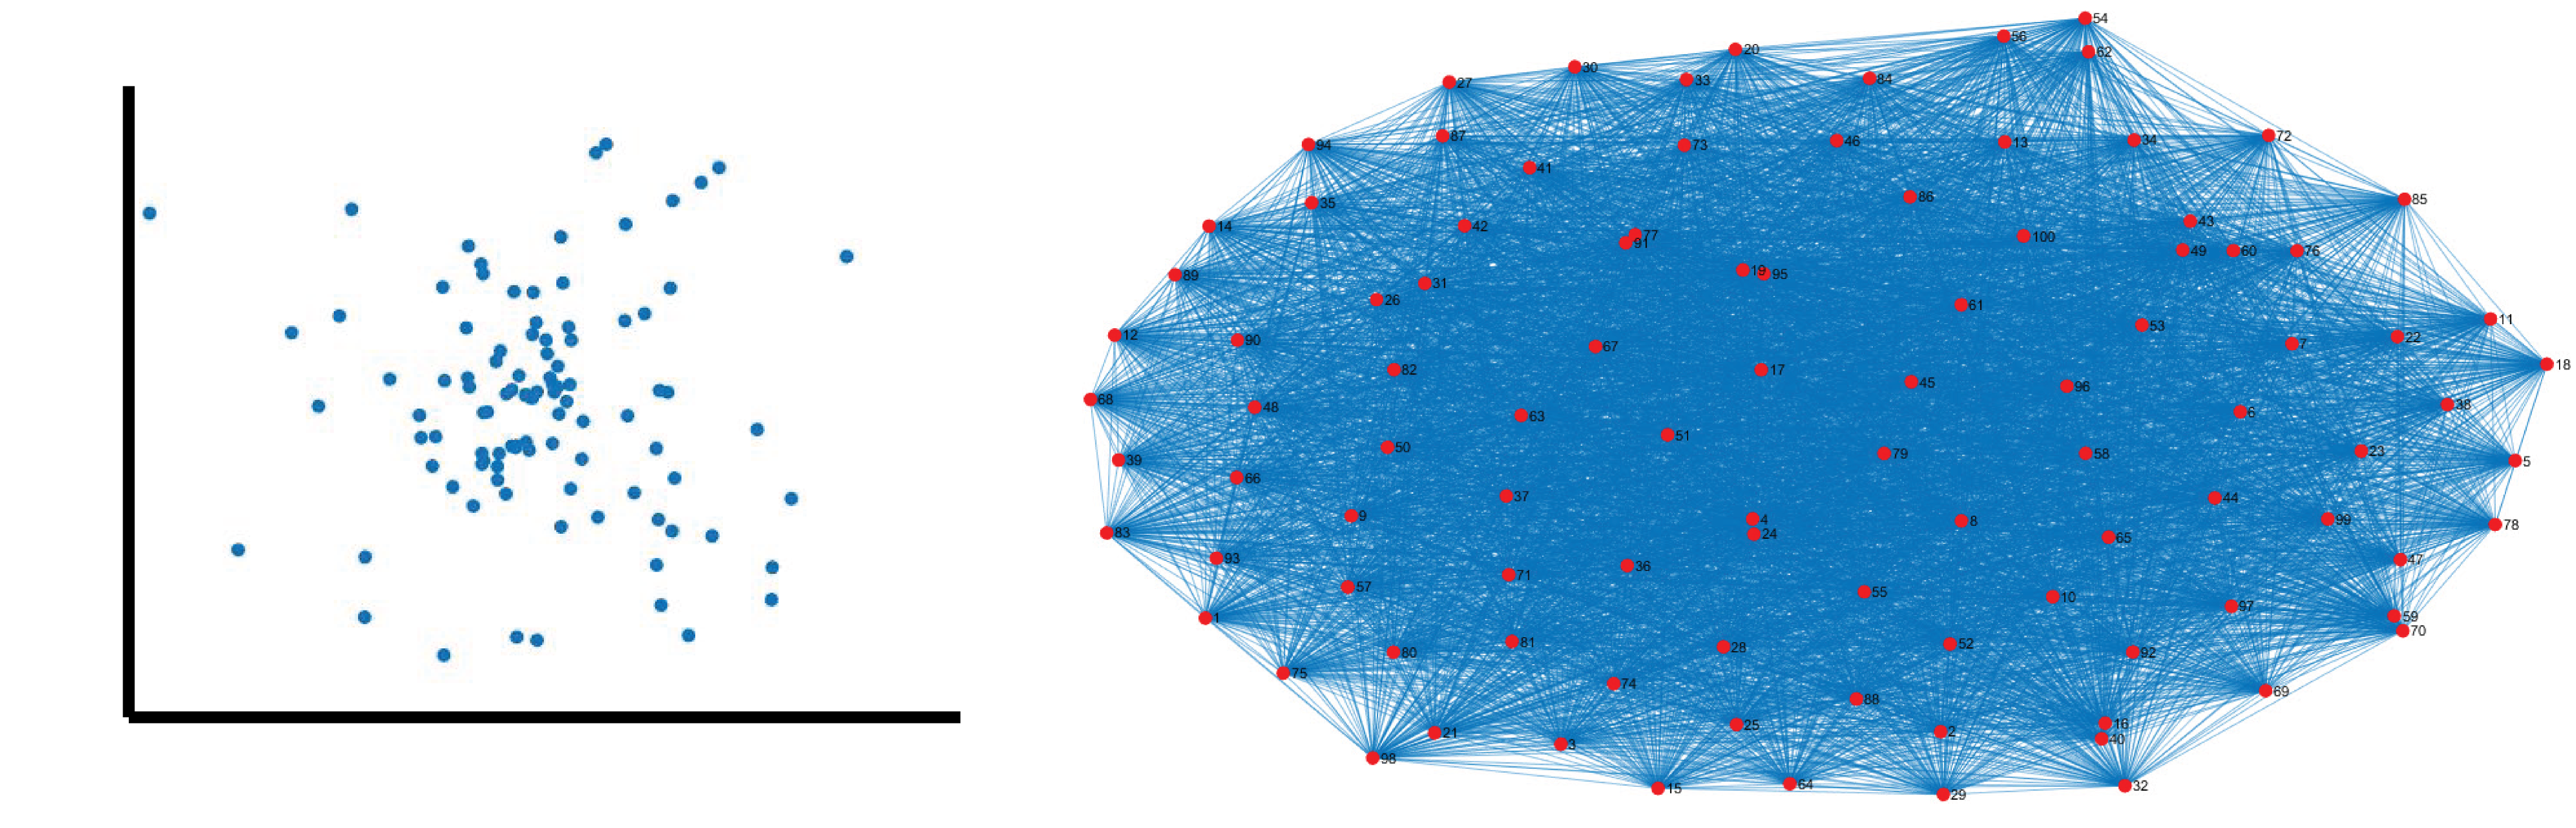
\includegraphics[width=\textwidth]{figures/MinSpTr}
	\end{figure}
	\vspace{5mm}
	\begin{itemize}[label={\MyShadow{$\bullet$}{blue!80}}]
		\item<2-> Subset of the edges that connects all the vertices together without any cycle and with the minimum weight. 
	\end{itemize}
	\vspace{20mm}
\end{frame}
\begin{frame}{The Density K-Means++ (DKM++) algorithm}
	\textbf{Minimum spanning tree}
	\begin{figure}[H]
		\centering
		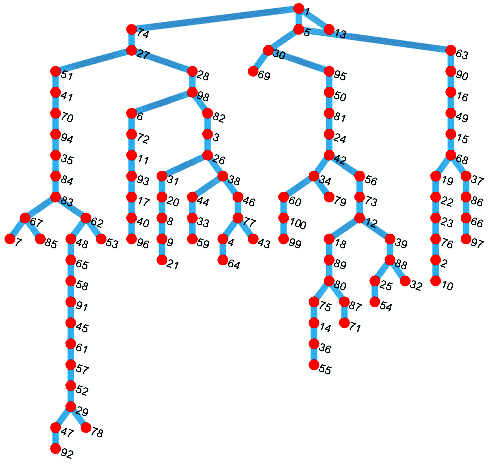
\includegraphics[width=0.65\textwidth]{figures/mstq}
	\end{figure}
\end{frame}
\begin{frame}{The Density K-Means++ (DKM++) algorithm}
	\textbf{Radius using MST-Heuristic}\\
	\vspace{10mm}
	\begin{multicols}{2}
	$\epsilon = 3 * IQR(L) + 75^{th} percentile(L)$,\\
	\vspace{2mm}
	$L \equiv$ MST weights (lengths)
	\vspace{10mm}
	\begin{figure}[H]
		\centering
		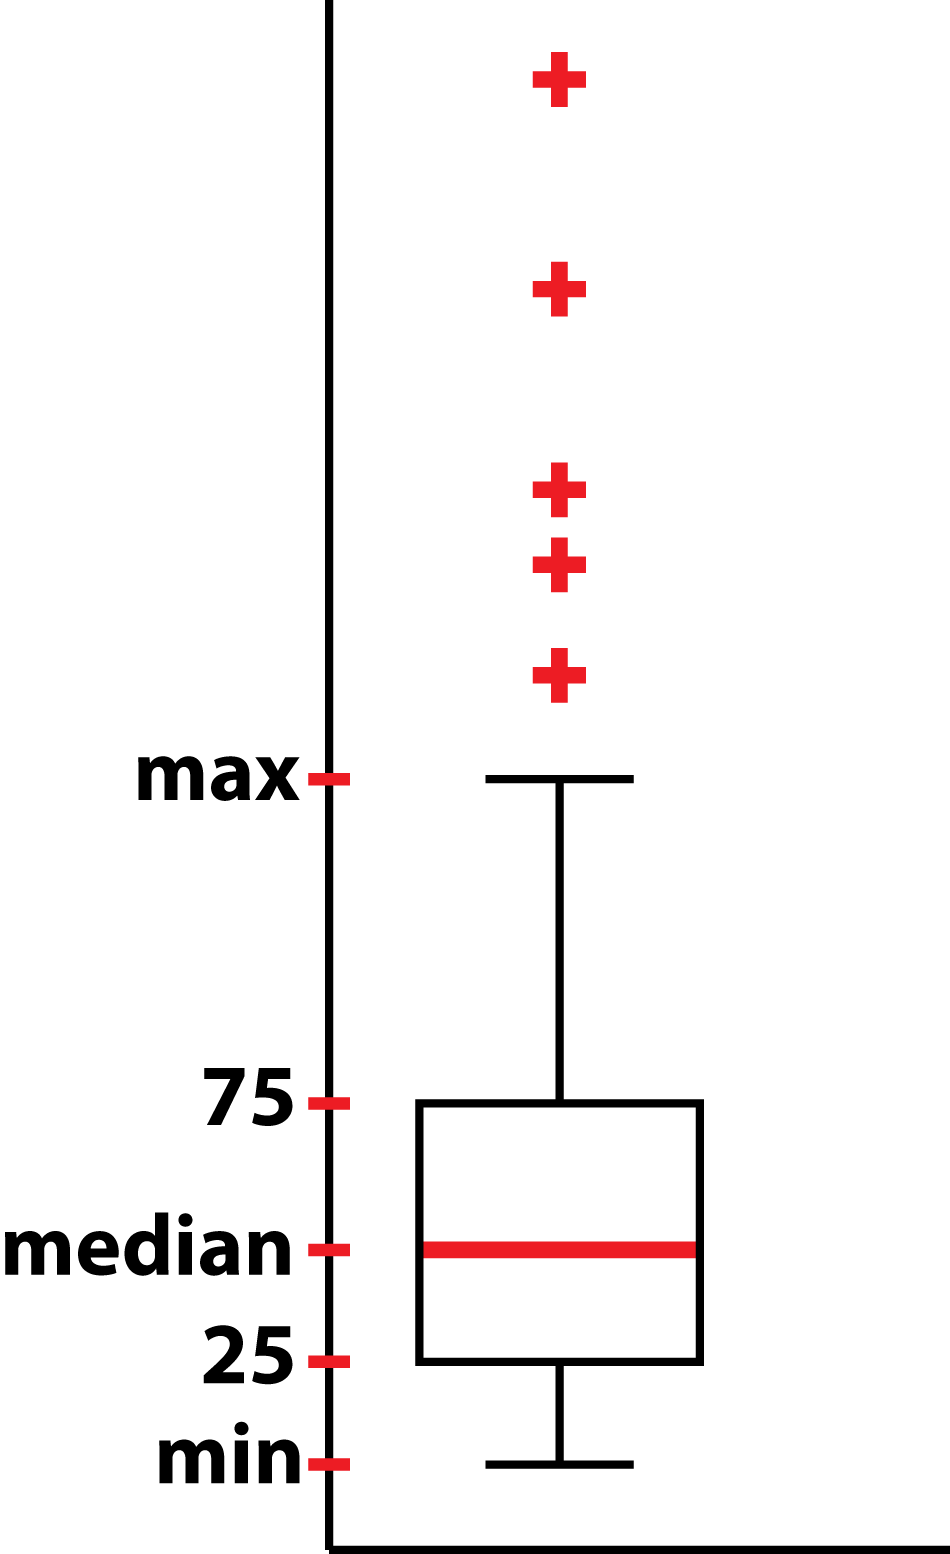
\includegraphics[width=0.3\textwidth]{figures/boxplot}
	\end{figure}		
	\end{multicols}
	\vspace{10mm}
\end{frame}

\begin{frame}{The Density K-Means++ (DKM++) algorithm}
	\textbf{Local density}\\
	\begin{itemize}[label={\MyShadow{$\bullet$}{blue!80}}]
		\item Find the $\epsilon-neighbors(x_i)$.
		\item Compute the local density $$\rho(x_i) = \sum_{y \in \epsilon-neighbors(x_i)} exp(\frac{-\lVert x_i - y_j \rVert}{\epsilon})$$
	\end{itemize}
	\begin{figure}[H]
		\centering
		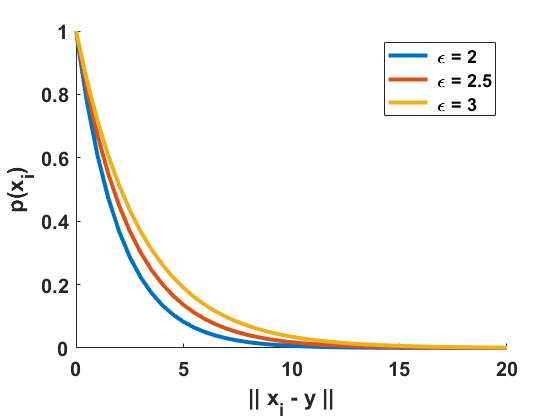
\includegraphics[width=0.59\textwidth]{figures/rho}
	\end{figure}
\end{frame}

\begin{frame}{The Density K-Means++ (DKM++) algorithm}
	\textbf{Prospectiveness}\\
	\vspace{15mm}
	\begin{itemize}[label={\MyShadow{$\bullet$}{blue!80}}]
		\item $C \longleftarrow \{max(\rho(x))\}$.
		\vspace{3mm}
		\item $\phi(x_j) = \rho(x_j) * \lVert x_j - x_m \rVert$, $x_m$ is the nearest data point added in $C$.
		\vspace{3mm}
		\item $C \longleftarrow \{max(\rho(x)),max(\phi(x))\}$
		\vspace{3mm}
		\item Repeat least 2 steps until k centroids are picked.
	\end{itemize}
	\vspace{40mm}
\end{frame}

\begin{frame}{The Density K-Means++ (DKM++) algorithm}
	\begin{figure}[H]
		\centering
		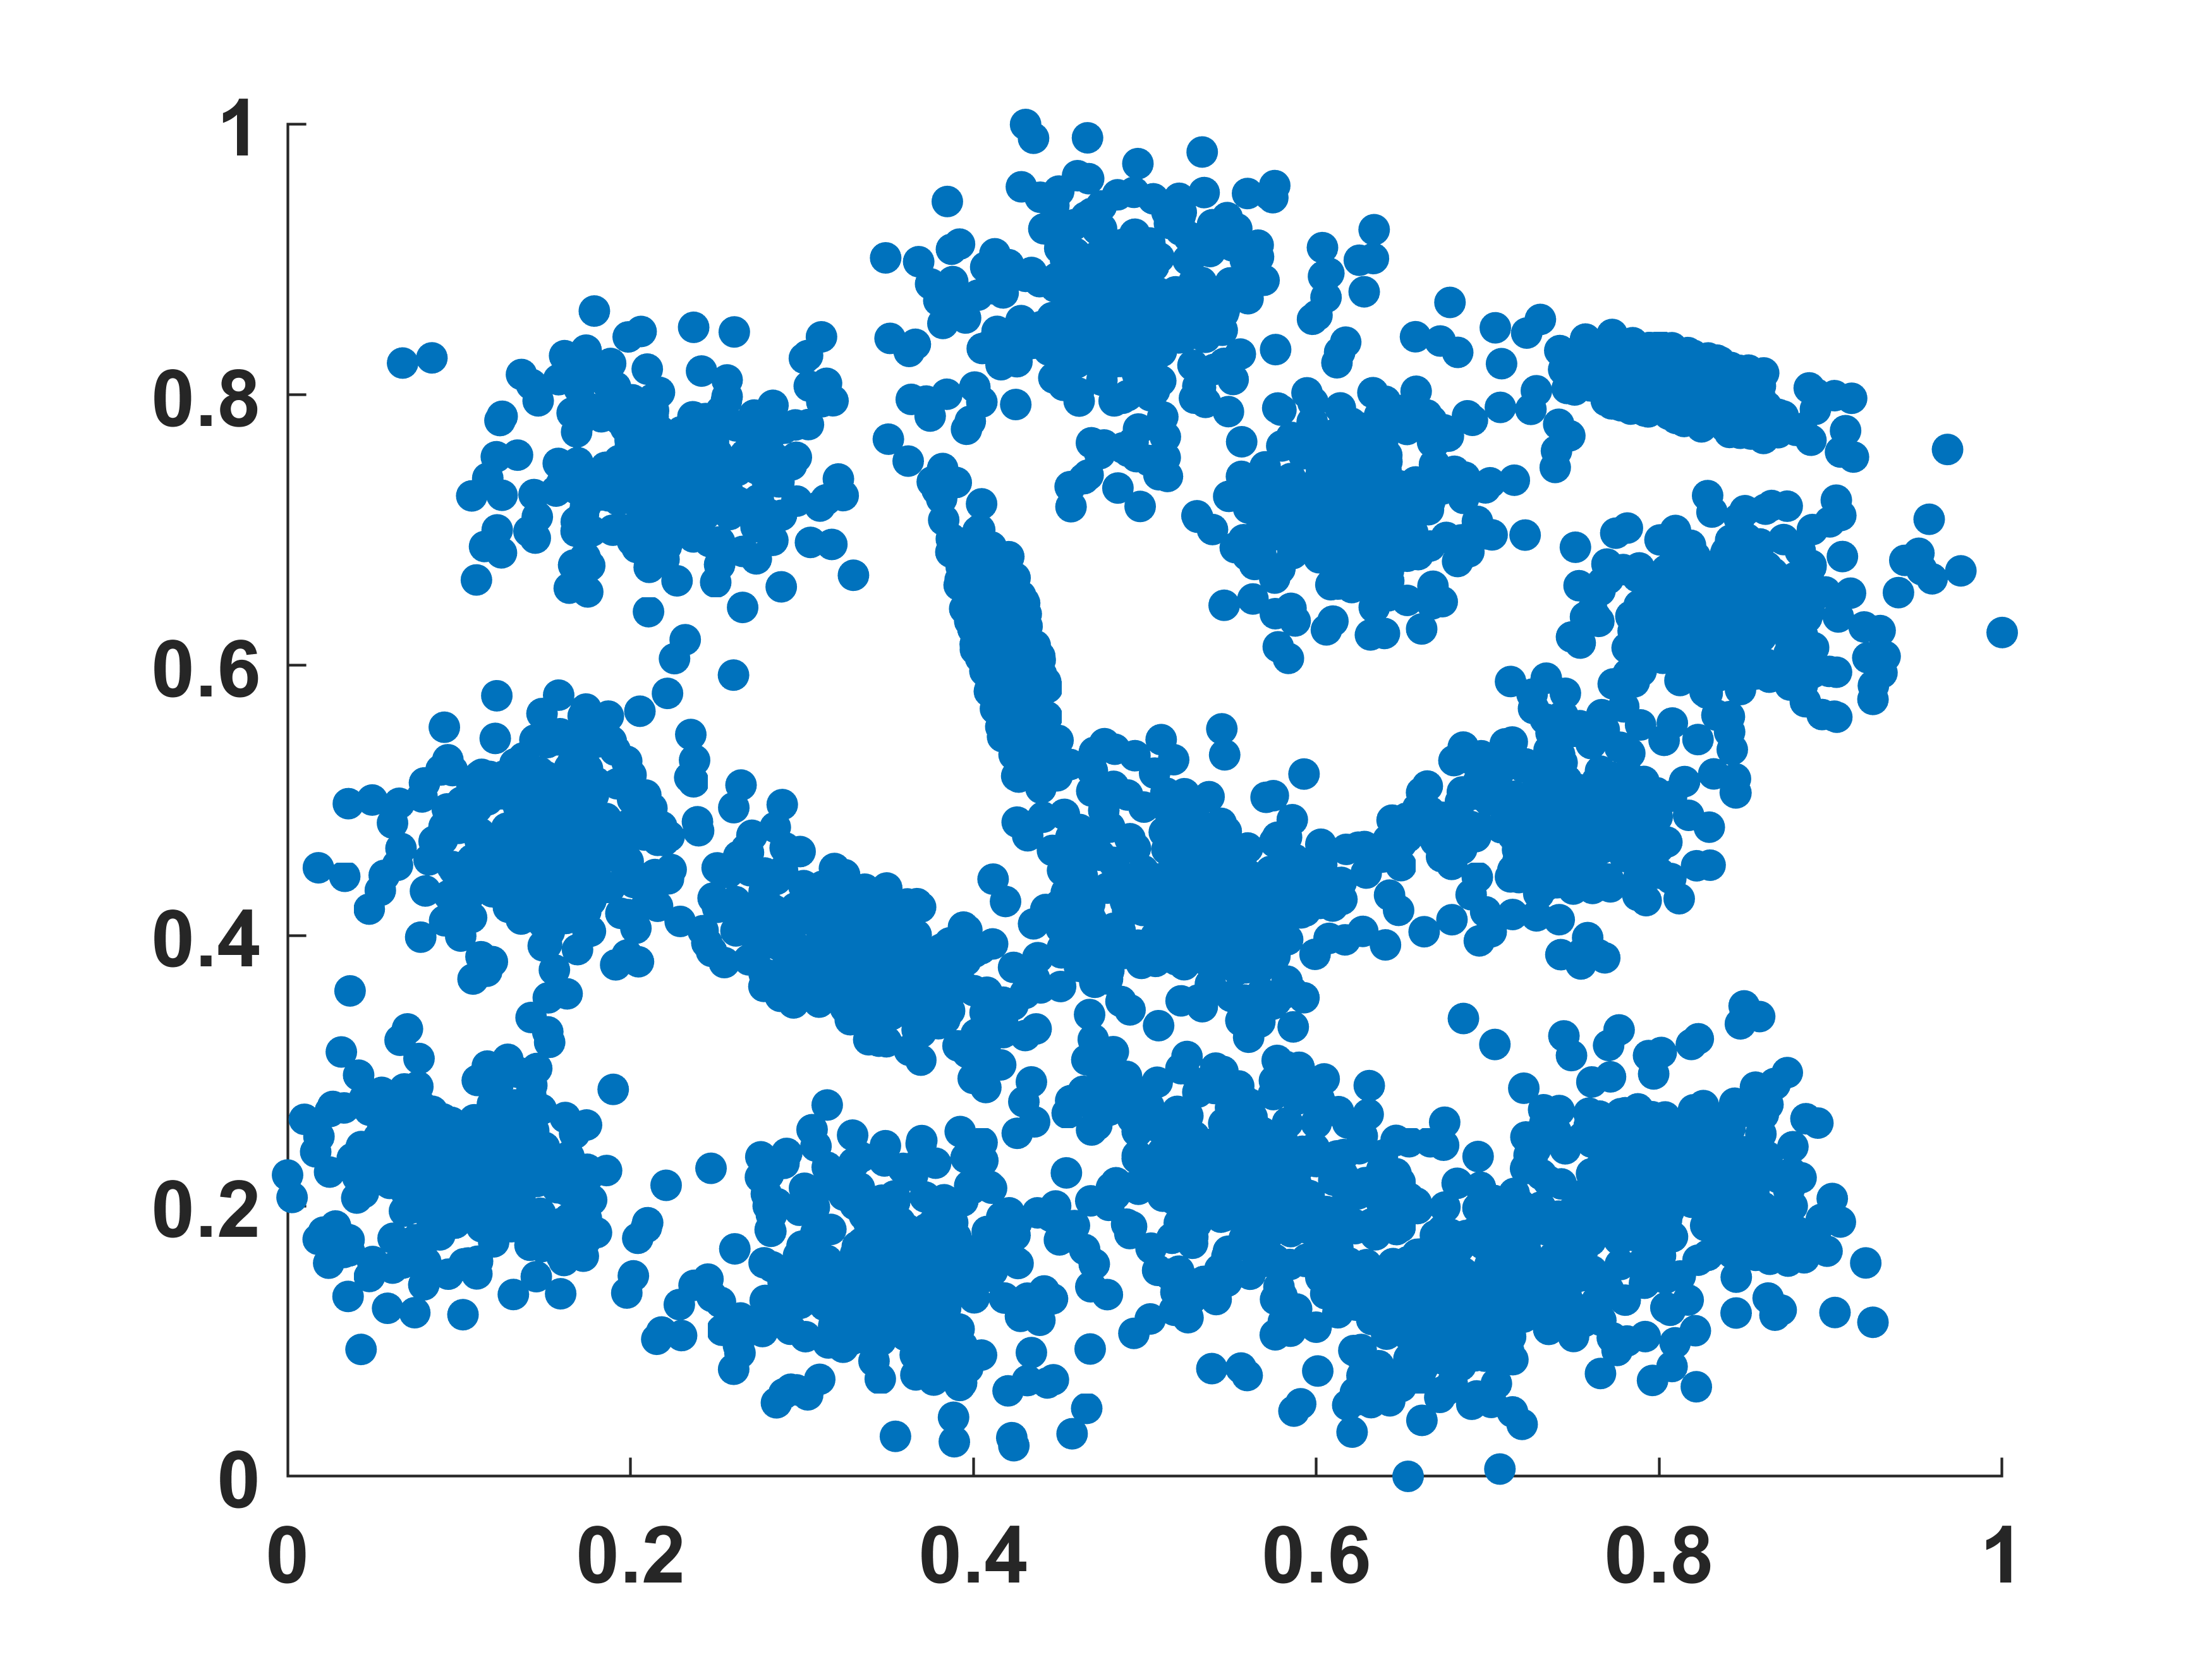
\includegraphics[width=0.56\textwidth]{figures/dataset}
	\end{figure}
\end{frame}
\begin{frame}{The Density K-Means++ (DKM++) algorithm}
	\begin{figure}[H]
		\centering
		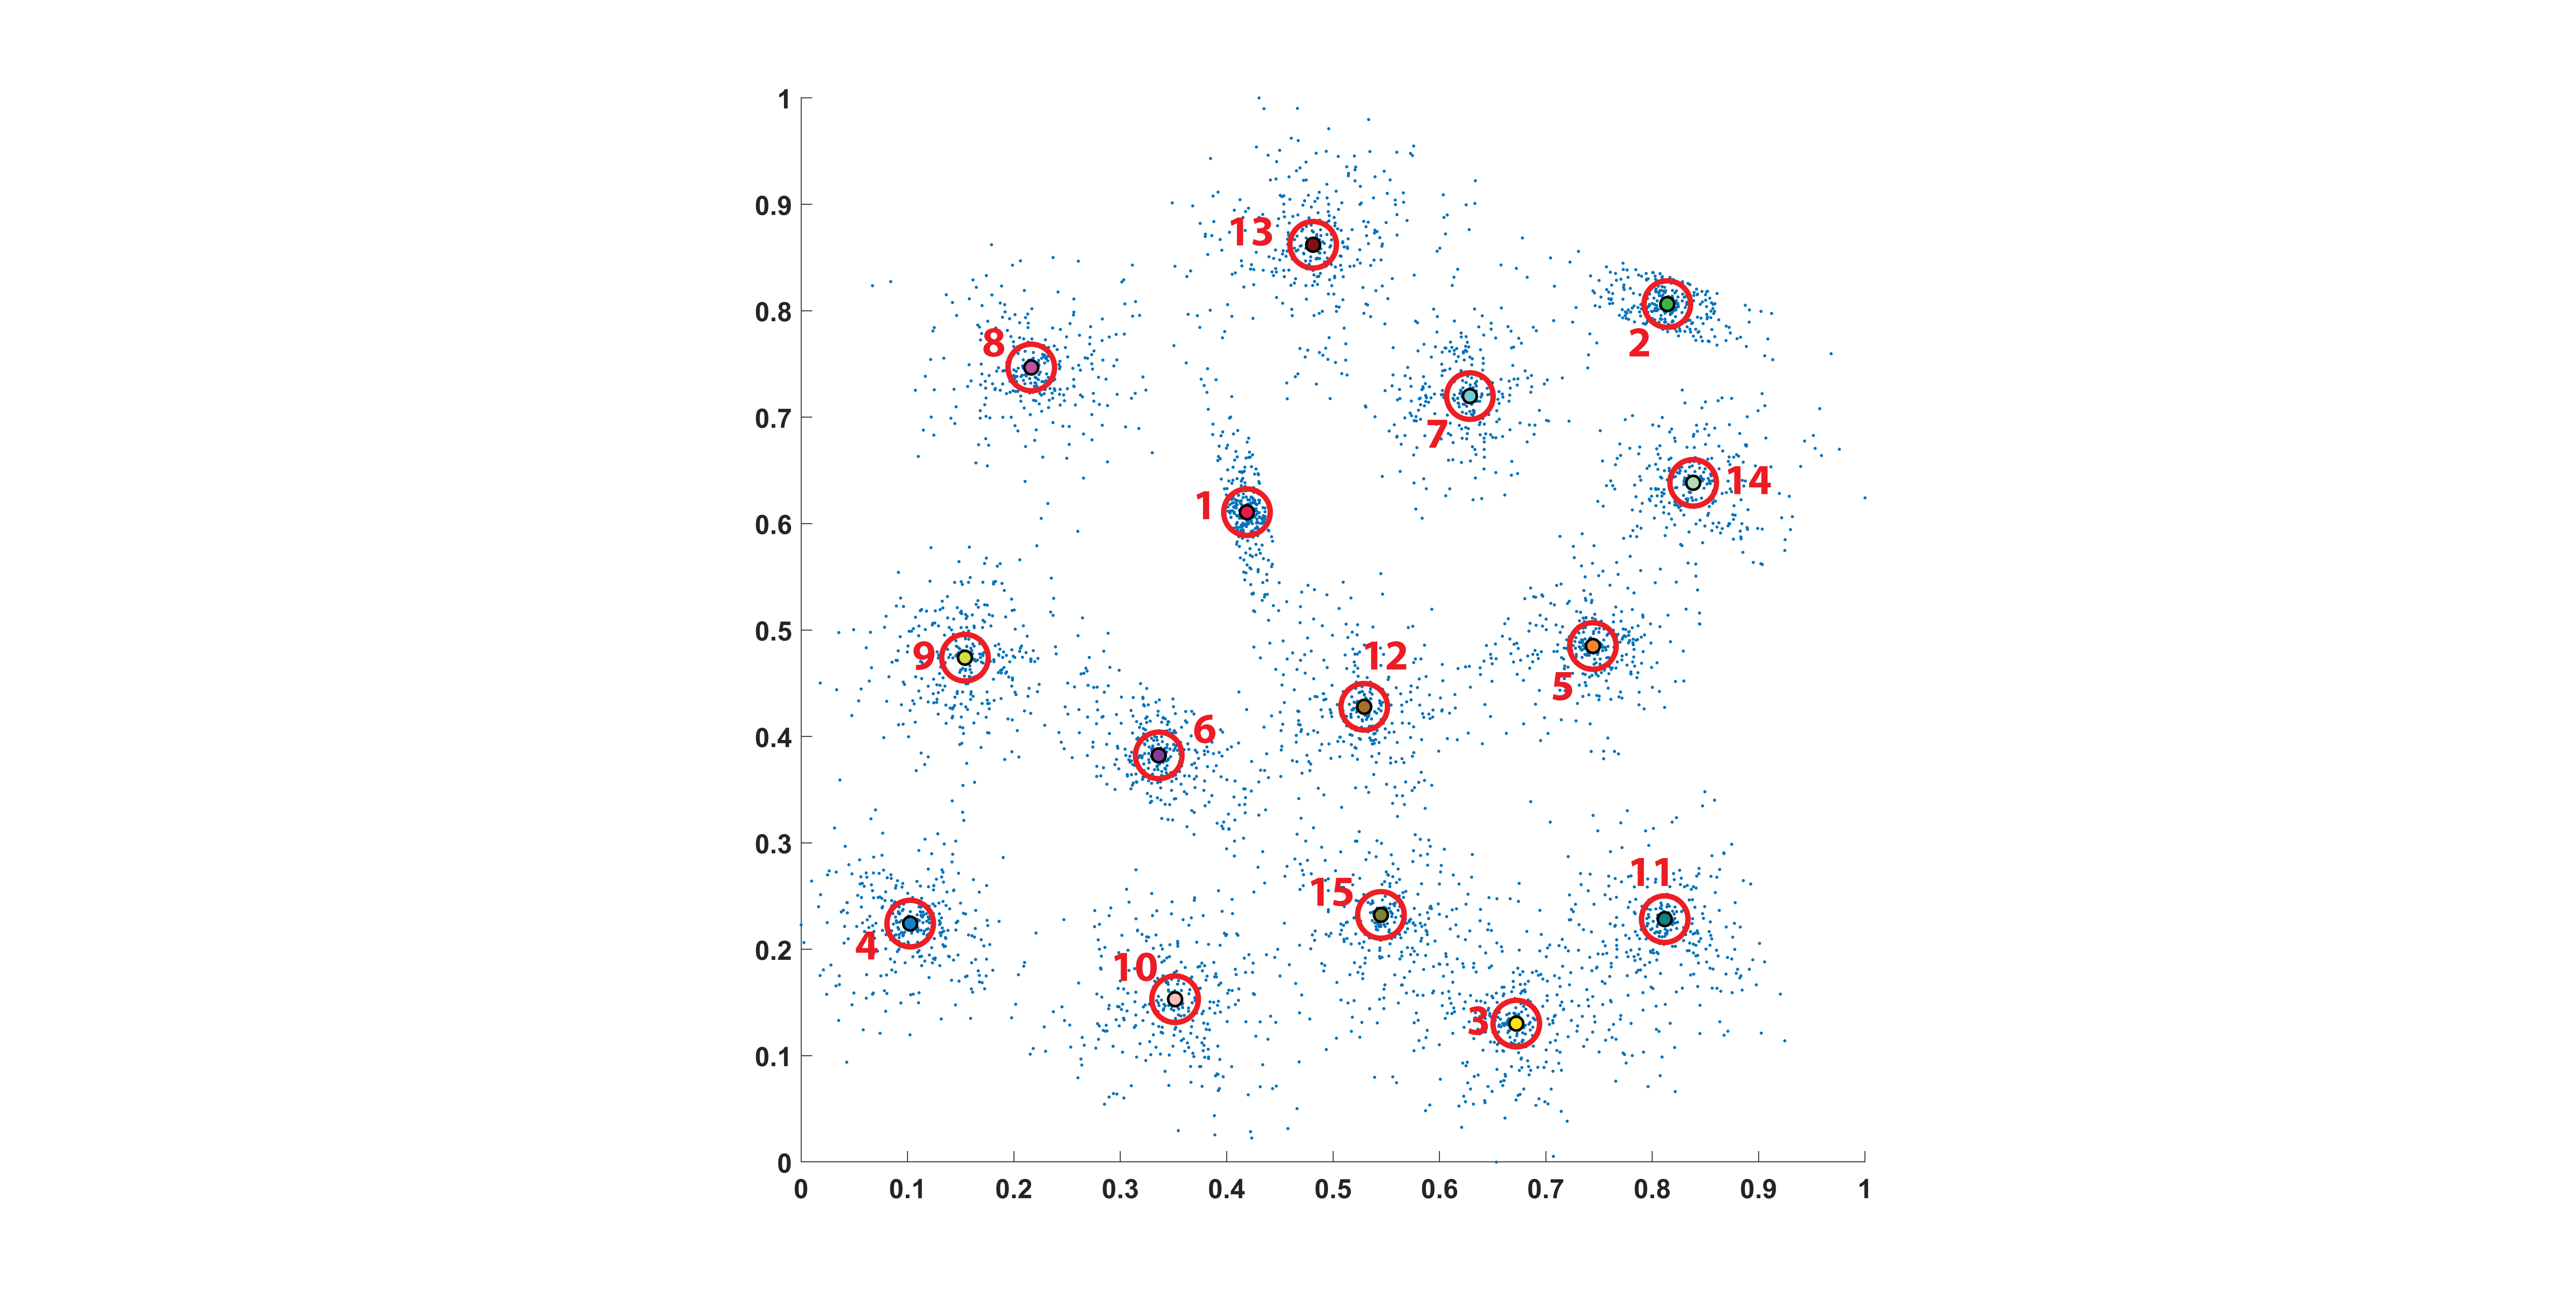
\includegraphics[width=\textwidth]{figures/dkmpp2a}
	\end{figure}
\end{frame}

}


\end{document}


%%%%%%%%%%%

% P = target distribution
% Distance: maximum mean discrepancy
% Lipschitz
% Frechet Inception Distance


